% !TEX program = xelatex % (can also use "lualatex")
\documentclass[12pt,a4paper]{report}
%-- Additions for this dissertation (the lines above and below this block follow the official template)
% PDF/A-2b output for the final file, as the University requires, with metadata in dissertation.xmpdata.
% XeTeX has no creation-date primitive, so the date is built from the compile date (noon, UTC) before pdfx needs it.
\makeatletter\ifdefined\pdfcreationdate\else\edef\pdfx@tmpdate{D:\the\year\two@digits\month\two@digits\day 120000+00'00'}\edef\pdfcreationdate{\expandafter\detokenize\expandafter{\pdfx@tmpdate}}\fi\makeatother
\usepackage{xcolor}
\usepackage[a-2b]{pdfx}
\usepackage{dissertation}
% Built-in sorting, so the acronym list appears without running makeglossaries (Tectonic, Prism).
\makenoidxglossaries
\makeindex
\usepackage{booktabs}
\newcommand{\minus}{\scalebox{0.75}[1.0]{$-$}}
\usepackage{tikz}
\usetikzlibrary{arrows.meta,positioning,calc,fit,shapes.geometric,patterns}
\usepackage{pgfplots}
\pgfplotsset{compat=1.18}
\usepgfplotslibrary{groupplots}
% Floats, diagrams and listings use single spacing, as the 1.5 body spacing made table rows and diagram boxes too tall.
\usepackage{etoolbox}
\usepackage{array}
\usepackage{placeins}
\AtBeginEnvironment{table}{\linespread{1}\selectfont}
\AtBeginEnvironment{figure}{\linespread{1}\selectfont}
\AtBeginEnvironment{tikzpicture}{\linespread{1}\selectfont}
\AtBeginEnvironment{lstlisting}{\linespread{1}\selectfont}
\captionsetup{font={small}}
% Ragged-right paragraph columns, because justified p{} cells stretched words apart in narrow columns.
\newcolumntype{L}[1]{>{\raggedright\arraybackslash}p{#1}}
\newcolumntype{C}[1]{>{\centering\arraybackslash}p{#1}}
\setlength{\tabcolsep}{5pt}
% Extra stretch so that long code identifiers do not push lines into the margin.
\setlength{\emergencystretch}{2em}
% A fourth heading level below subsubsection, printed as an unnumbered run-in title.
\makeatletter
\titleclass{\subsubsubsection}{straight}[\subsection]
\newcounter{subsubsubsection}[subsubsection]
\renewcommand\thesubsubsubsection{\thesubsubsection.\arabic{subsubsubsection}}
\def\toclevel@subsubsubsection{4}
\def\l@subsubsubsection{\@dottedtocline{4}{8em}{4em}}
\makeatother
\setcounter{secnumdepth}{4}
\titleformat{\subsubsubsection}[runin]{\normalfont\normalsize\bfseries}{}{0pt}{}[.]
\titlespacing*{\subsubsubsection}{0pt}{2ex plus .5ex minus .2ex}{0.6em}
\titleformat{\paragraph}[runin]{\normalfont\normalsize\bfseries}{}{0pt}{}
\titlespacing*{\paragraph}{0pt}{1.5ex plus .5ex minus .2ex}{0.6em}
% Let floats share pages with text instead of forcing near-empty float pages.
\renewcommand{\topfraction}{0.85}
\renewcommand{\bottomfraction}{0.6}
\renewcommand{\textfraction}{0.1}
\renewcommand{\floatpagefraction}{0.75}
\setcounter{topnumber}{3}
\setcounter{bottomnumber}{2}
\setcounter{totalnumber}{4}
% Do not prefer a page break before section headings (with ragged bottoms this left pages a third empty).
\makeatletter\@secpenalty=0\makeatother
% Table rows generated by analysis/analyze.py, read with the primitive input so that booktabs rules work inside tabular.
\makeatletter
\newcommand{\tabinput}[1]{\@@input #1 }
\makeatother
\lstset{captionpos=b,basicstyle=\ttfamily\footnotesize,columns=fullflexible,keepspaces=true,breaklines=true,frame=single,rulecolor=\color{black!35},showstringspaces=false}
\lstdefinelanguage{XML}{morestring=[b]",morecomment=[s]{<!--}{-->},stringstyle=\color{black!70},identifierstyle=\color{black},keywordstyle=\bfseries}
% Placeholder for a screenshot the author will capture: \shotplaceholder[height]{file name}{what the image must show}
\newcommand{\shotplaceholder}[3][6.5cm]{%
  \begin{tikzpicture}
    \node[draw=black!45, fill=black!5, dashed, line width=0.6pt, minimum width=0.95\textwidth, minimum height=#1,
          text width=0.85\textwidth, align=center, inner sep=8pt]
      {{\bfseries SCREENSHOT TO ADD}\\[3pt]{\small\ttfamily images/shots/\detokenize{#2}}\\[6pt]{\small #3}};
  \end{tikzpicture}}
% Tables use a full grid with a shaded header row and merged group cells (converted by analysis/grid_style.py).
\usepackage{colortbl}
\usepackage{multirow}
\definecolor{headgray}{HTML}{E6E7E8}
\definecolor{groupgray}{HTML}{F4F5F6}
\arrayrulecolor{PANTONECoolGray7C}
\AtBeginEnvironment{table}{\renewcommand{\arraystretch}{1.2}}
% Chart colors from the Okabe-Ito palette, which stays distinguishable for color-blind readers.
\definecolor{cBlue}{HTML}{0072B2}
\definecolor{cOrange}{HTML}{E69F00}
\definecolor{cGreen}{HTML}{009E73}
\definecolor{cVerm}{HTML}{D55E00}
\definecolor{cSky}{HTML}{56B4E9}
\definecolor{cPurple}{HTML}{CC79A7}
% The same colors mark the same concepts in every chart and diagram, the UML class and state diagrams included:
% purple for the schedule and lateness, vermilion for queueing, blue for walking and paths, green for service and the
% environment, orange for the person and the combined steering, sky blue for perception and recording, and grey for setup.
% Acronyms used in the dissertation (\gls{key}).
\newacronym{abm}{ABM}{agent-based model}
\newacronym{ai}{AI}{artificial intelligence}
\newacronym{csv}{CSV}{comma-separated values}
\newacronym{cpu}{CPU}{central processing unit}
\newacronym{dul}{DUL}{Daily Urban Life}
\newacronym{fifo}{FIFO}{first in, first out}
\newacronym{fps}{FPS}{frames per second}
\newacronym{fsm}{FSM}{finite-state machine}
\newacronym{gpu}{GPU}{graphics processing unit}
\newacronym{odd}{ODD}{Overview, Design concepts, and Details}
\newacronym{orca}{ORCA}{optimal reciprocal collision avoidance}
\newacronym{pdr}{PDR}{Preliminary Dissertation Report}
\newacronym{rvo}{RVO}{reciprocal velocity obstacles}
\newacronym{soa}{SOA}{State of the Art}
\newacronym{ue}{UE}{Unreal Engine}
\newacronym{xml}{XML}{Extensible Markup Language}

% Month names with a capital letter on the covers and statements, as the University's rules require.
\def\myear{\ifcase\month\or
 January\or February\or March\or April\or May\or June\or
 July\or August\or September\or October\or November\or December\fi
 \space\number\year}
%-- End of additions

%\logo{EAAD}{School of Architecture, Art and Design}{}
%\logoB{EAAD}{School of Architecture, Art and Design}{}

%\logo{EC}{School of Sciences}{}
%\logoB{EC}{School of Sciences}{}

%\logo{ED}{Law School}{}
%\logoB{ED}{Law School}{}

\logo{EE}{School of Engineering}{}
\logoB{EE}{School of Engineering}{}

%\logo{EEG}{School of Economics and Management}{}
%\logoB{EEG}{School of Economics and Management}{}

%\logo{ELACH}{School of Letters, Arts and Human Sciences}{}
%\logoB{ELACH}{School of Letters, Arts and Human Sciences}{}

%\logo{EM}{Medical school}{}
%\logoB{EM}{Medical school}{}

%\logo{EP}{School of Psychology}{}
%\logoB{EP}{School of Psychology}{}

%\logo{ESE}{Higher School of Nursing}{}
%\logoB{ESE}{Higher School of Nursing}{}

%\logo{I3Bs}{Research Institute on Biomaterials,}{Biodegradables and Biomimetics}
%\logoB{I3Bs}{Research Institute on Biomaterials,}{Biodegradables and Biomimetics}

%\logo{ICS}{Institute of Social Sciences}{}
%\logoB{ICS}{Institute of Social Sciences}{}

%\logo{IE}{Institute of Education}{}
%\logoB{IE}{Institute of Education}{}

\author{Rui Filipe Pimenta Armada}

\titleA{Authoring Pedestrian Activities with}
\titleB{Capacity-Aware Stations and Hybrid Boids}
%\titleC{Title Title Title Title}

\masters{Master’s Dissertation in Informatics Engineering}
%\area{Area of specialization}
\supervisor{Professor Doctor António José Borba Ramires Fernandes}
%\cosupervisor{Co-Supervisor Name}

\bibpunct[,]{(}{)}{;}{a}{,}{,}
\begin{document}
\setlength{\parindent}{0em}

%-- Covers
\begin{titlepage}
\color{PANTONECoolGray7C}
\raggedright
\thelogo
\leading{20.4pt}
{\Large
\theauthor
\\[20.4pt]
\textbf{\thetitleA}
\\
\textbf{\thetitleB}
\\
\textbf{\thetitleC}
}

\vspace*{\fill}
{\footnotesize \myear}
\end{titlepage}

\null
\thispagestyle{empty}
\pagecolor{PANTONECoolGray7C}
\afterpage{\nopagecolor}
\newpage

\begin{titlepage}
\color{PANTONECoolGray7C}
\raggedright
\thelogoB
\leading{20.4pt}
{\Large
\theauthor
\\[20.4pt]
\textbf{\thetitleA}
\\
\textbf{\thetitleB}
\\
\textbf{\thetitleC}
}

\vspace{55.2mm}
\leading{16.8pt}
{\large
\themasters
\thearea
Work supervised by
\\
\textbf{\thesupervisor}
\\
\thecosupervisor}

\vspace*{\fill}
{\footnotesize \myear}
\end{titlepage}

%-- Document setup
\newgeometry{right=25mm, left=25mm, top=25mm, bottom=25mm}
\pagenumbering{roman}
% RT-80/2026: the title page is counted but not numbered, so the next page is ii.
\setcounter{page}{2}

\setlength{\parskip}{0pt}
\setlength{\parindent}{1.5em}

%-- Preamble
\chapter*{Copyright and Terms of Use for Third Party Work}
\setlength{\parskip}{1em}
\noindent
This dissertation reports on academic work that can be used by third parties as long as the internationally accepted standards and good practices are respected concerning copyright and related rights.

\noindent
This work can thereafter be used under the terms established in the license below.

\noindent
Readers needing authorization conditions not provided for in the indicated licensing should contact the author through the RepositóriUM of the University of Minho.

\section*{License granted to users of this work:}

\noindent

\includegraphics[]{images/CCBY.png}
\\
\textbf{CC BY}
\\
\url{https://creativecommons.org/licenses/by/4.0/}



\setlength{\parskip}{0em}
\chapter*{Acknowledgements}
\setlength{\parskip}{1em}

Agradeço ao meu orientador, Professor António José Borba Ramires Fernandes, pelo acompanhamento atento nesta última etapa académica e pela paciência, conhecimento, bom humor e exemplo profissional que me deu desde a licenciatura. Levo comigo a sua exigência e a sua paixão pela computação gráfica.

Às pessoas mais importantes da minha vida, obrigado. Ao meu pai, Rui, que sempre me apoiou e me mostrou o que é a integridade e força. À minha irmã, Carolina, a voz da razão que me acolheu nos momentos mais difíceis. E à minha mãe, Paula, o meu maior amor, que me trouxe calma e sempre foi a minha fã número um. Só cheguei aqui porque lutámos juntos, e esta conquista é tanto vossa como minha. Agradeço também aos familiares que acompanharam esta viagem, mas, se começasse a escrever nomes, nunca mais daqui saía.

Aos meus amigos, companheiros de batalha passados e futuros, obrigado por tudo o que me ensinaram. Ao Carlos António, o irmão que nunca tive desde o 2.º ano da licenciatura: que venham muitos mais anos. À Márcia Teixeira e à Sofia Marques, as minhas amigas lindas, que prezo mais do que ninguém: nunca saberei retribuir o que fizeram por mim. Agradecer à Bea, ao Miguel, à Filipa, à Morgana, ao Artur, ao Dinis, ao Rui e ao Zé. Sois todos uma bênção que levo no coração para sempre.

Dedico esta dissertação a cinco pessoas. Quatro já não estão entre nós, mas sinto as suas mãos nos meus ombros enquanto escrevo. À minha avó Lia, que continua ao meu lado e me ensinou a ser casmurro e a persistir. Ao meu avô Nelinho, que me inspirou a deixar sempre um bom nome, porque o mundo precisa de mais pessoas boas. Ao meu avô Pimenta, que me ensinou a ser ambicioso e a apontar para as estrelas, por mais impossível que pareça. À minha avó Dina, um dos grandes amores da minha vida, que me deu amor incondicional e cuja falta não se descreve por palavras. E à minha querida Zinda, a minha “criança grande”, a estrelinha dos meus olhos, que me ensinou a viver com leveza, alegria e pela qual sinto falta todos os dias. Amo-vos aos cinco e daria tudo para estarmos todos juntos mais uma vez.

\setlength{\parskip}{0em}

\chapter*{Statement of Integrity}
\setlength{\parskip}{0.8em}
\noindent
I hereby declare having conducted this academic work with integrity.

\noindent
I confirm that I have not used plagiarism or any form of undue use of information or falsification of results along the process leading to its elaboration.

\noindent
I further declare that I have fully acknowledged the Code of Ethics and Conduct of the University of Minho.

\section*{Declaration on the Use of Artificial Intelligence (AI) Tools}

\noindent
I hereby declare having acted this academic work with integrity and confirm that I have not resorted to any form of undue use of AI tools, nor to the falsification or omission of information, sources, data, results or processes in any of the stages leading to its elaboration.

\noindent
I further declare that any use of AI tools was done in a transparent and responsible manner, being duly noted in the work, and that I critically verified the accuracy of the content produced with their support, assuming full responsibility for what I submit.

\noindent
I further declare that I have fully acknowledged the Code of Ethics and Conduct of the University of Minho, as well as the applicable standards of academic integrity and data protection.

\noindent
AI tools were used in this work as follows: Claude and Grammarly helped with grammar, language revision and punctuation, and Claude also helped with the test and analysis scripts and with automating their runs.

\noindent
University of Minho, Braga, \myear

\vspace{20mm}
\noindent\theauthor
\setlength{\parskip}{0em}

\chapter*{Resumo}

\noindent\textbf{Autoria de atividades pedonais com estações sensíveis à capacidade e boids híbridos}

Muitas perguntas sobre edifícios e espaços públicos dependem do que as pessoas precisam, como uma secretária ou uma mesa, e do que acontece quando outra pessoa precisa dele ao mesmo tempo. Uma simulação que lhes responda tem de mostrar quando cada atividade começa de facto e porque se atrasa. Esta dissertação propõe uma estrutura em que horários em XML indicam quem faz o quê e quando, estações com capacidade limitada, fila e tempo de serviço decidem quando cada atividade ocorre, e uma camada de movimento híbrida segue caminhos de navegação, que os boids apenas desviam ligeiramente. Uma hora definida é, assim, um pedido, cujo início real depende do que a pessoa ainda faz, da distância e da disponibilidade do recurso, e um registo de regras, visitas e caminhadas explica cada atraso.

Implementámos a estrutura em C++ na Unreal Engine 5.4, com uma única implementação de pessoa numa rotina urbana diária com 50 pessoas, em dois centros comerciais, numa evacuação e em corredores de fluxo dirigido, com apenas uma ação nova em todos os cenários. Com a marcha e o relógio sincronizados, a avaliação mediu a origem da diferença entre os tempos definidos e os realizados. A espera por estações partilhadas dominou essa diferença nos centros comerciais, onde as filas foram 76\% do atraso no início das regras de estação e 92\% numa hora de almoço com um lugar por balcão, enquanto na rotina diária pesaram mais as caminhadas longas até destinos congestionados. As mudanças de capacidade comportaram-se como uma sequência de filas: em 30 execuções por configuração, um segundo ou terceiro lugar nas mesas reduziu a mediana da espera por visita de 0,84 para 0,51 minutos simulados, enquanto mais lugares nos balcões apenas deslocaram a fila para as mesas, como se viu na hora de almoço, com esperas de vários minutos. Estas tendências mantiveram-se com dois passos, mas não a sua dimensão. Os boids espalharam os grupos em dois de três corredores e aliviaram um estrangulamento, e um só computador anima 50 a 100 pessoas com uma média acima de 30 imagens por segundo, embora as mais lentas fiquem abaixo desse valor. Sem validação com peões reais, os resultados descrevem o modelo, não edifícios reais.

\paragraph{Palavras-chave} Autoria de regras, Boids, Recursos partilhados, Simulação de multidões, Unreal Engine

\cleardoublepage

\chapter*{Abstract}

\noindent\textbf{Authoring Pedestrian Activities with Capacity-Aware Stations and Hybrid Boids}

Many questions about buildings and public spaces are about what people need, such as a desk or a table, and what happens when someone else needs it at the same time. A simulation that answers them must show when each activity really starts and why it starts later than planned. This thesis presents a rule-authoring framework for pedestrian activities, in which XML schedules state who does what and from when, stations with a limited capacity, a first-come, first-served queue and a service time decide when each activity can take place, and a hybrid movement layer follows navigation paths while the boids forces only turn the heading slightly. An authored time is therefore a request, whose actual start depends on what the person is still doing, how far they must walk and whether the resource is free, and a recorder logs every rule, visit and walk to explain each delay.

We built the framework in C++ in Unreal Engine 5.4 and used one implementation of a person for a daily urban routine with 50 people, two shopping center layouts, an emergency evacuation and a set of directed-flow corridors, with only one new action across all scenarios. With walking and the clock advancing together, the evaluation measured where the gap between authored and realized times comes from. Waiting for shared stations was the largest part of that gap in the shopping centers, where queueing made up 76\% of the start delay of station rules and 92\% in a lunch rush with one place per counter, while in the daily routine long walks to crowded target points took a larger share. Capacity changes behaved as a pipeline of queues: over 30 runs per setting, a second or third place at the food tables lowered the median wait per station visit from 0.84 to 0.51 simulated minutes, while extra places at the food counters only moved the queue to the tables, and the lunch rush showed the same shift with waits of several minutes. These directions held at two frame steps, although their sizes changed. The boids blend spread the cohorts in two of three test corridors and eased a bottleneck, and one desktop computer animates 50 to 100 people at a mean above 30 frames per second, although its slowest frames fall below that. Without validation against real pedestrians, the results describe the model rather than real buildings.

\paragraph{Keywords} Boids, crowd simulation, rule authoring, shared resources, Unreal Engine

\cleardoublepage


\phantomsection
\tableofcontents

% Acronyms (RT-80/2026 lists abbreviations and acronyms right after the contents)
\printnoidxglossary[type=\acronymtype,nonumberlist,sort=word,title={Acronyms}]

\cleardoublepage
\listoffigures

% List of tables
\renewcommand*{\listtablename}{List of Tables}
\listoftables

\cleardoublepage
\pagenumbering{arabic}

%-- Dissertation
\part{Introductory Material}

\chapter{Introduction}\label{chap:intro}

Pedestrian simulations allow us to ask questions about a place before it is built or altered. Will the food court have enough tables during the lunch rush, will two shifts of office workers compete for the same desks, and will one of the exits become a choke point when the alarm sounds? The way people walk gives part of the answer, but the rest depends on why they move, what they are looking for when they get there and how the time spent waiting for one thing delays the next.

This dissertation studies how a simulation of purposeful pedestrians can show where and why the activities in a place start later than intended. Boids are well known for the emergent collective motion that results from a small number of local rules \citep{reynolds1987flocks}, and they are straightforward to incorporate into a game engine. The basic model, however, has nothing that would send one boid to work at 9 am or make another need a table at the food court. We developed a framework that treats purpose as data, so that the analysis of a place, that is, when each activity actually starts, how long people wait for shared resources and how a change in capacity affects the delays, can be extracted from recorded runs. To make such analyses cheap, the system is designed to describe different places with as little change to its code as possible, so a new study requires new schedules, maps and settings rather than new code. Schedules define who does what and when, a movement layer combines navigation paths with the bounded steering of the boids, stations with a finite capacity determine when an activity can start, and the environment constrains where people can go. We implemented the framework in \gls{ue} 5.4 with public source code, schedules and maps \citep{armada2026repository}, and the same implementation of a person simulates a daily urban routine, a shopping center, an emergency evacuation and a set of directed-flow corridors.

This chapter presents the motivation (\cref{sec:intro-motivation}), the research question and the objectives (\cref{sec:intro-goals}), and the structure of the document (\cref{sec:intro-structure}).

\section{Motivation and Context}\label{sec:intro-motivation}

\subsection{Crowds as an activity problem}\label{sub:intro-activity}

People in a station, a shopping center or an office are rarely just wandering about, as they are almost always on their way to buy a ticket, sit at a desk, have a meal or leave the building. Research into pedestrian behavior identifies three levels of decision: the strategic level, which plans the activities, the tactical level, which decides where to do them and which route to take, and the operational level, which is the walking itself and the avoidance of other people \citep{hoogendoorn2004pedestrian}.

Models of local motion work only at the operational level, as boids use separation, alignment and cohesion \citep{reynolds1987flocks}, and the social force model moves people toward their desired velocity while other people and walls push them away \citep{helbing1995social}. Reciprocal velocity models restrict each individual to the velocities that avoid a collision with its neighbors \citep{vandenberg2011reciprocal}. These models describe what happens once people have decided where to go, but they do not say what the destination is or what happens when the resource that a person needs is not available. Other work looks at the level of activities above locomotion. Autonomous pedestrians buy a ticket, queue and rest in a virtual train station \citep{shao2007autonomous}, the people of \citet{paris2009activity} carry out goal-oriented daily activities, and at the scale of a city, MATSim produces daily plans that link activities through trips \citep{horni2016matsim}.

Waiting depends on both capacity and demand: a food court (\cref{fig:intro-foodcourt}), for example, has a fixed number of counters and tables, so when demand exceeds capacity, people wait and their next activity is delayed. Queueing theory treats such resources as servers with a given capacity, an arrival process and a service time \citep{kendall1953stochastic,shortle2018fundamentals}. In a crowd simulation, the arrival process is derived from the individual schedules, the walking times and the earlier delays. A simulation that studies capacity must therefore model activities, resources and durations, and it must let waiting arise from these rather than impose it.

\subsection{From flocking demonstrations to authored studies}\label{sub:intro-authoring}

Reynolds breaks character behavior down into three layers: action selection, steering and locomotion \citep{reynolds1999steering}. Boids operate at the steering level, and a flocking demonstration needs little action selection, but as soon as a demonstration takes place in a particular location, action selection becomes the dominant issue. When each demonstration has its own controller, the code has to be rewritten for every combination of questions, such as a morning routine with fewer desks than workers or the same routine with an alarm going off. It is then difficult to tell whether the differences between runs come from the change under study or from the code written for that particular scenario.

\begin{figure}[H]
\centering
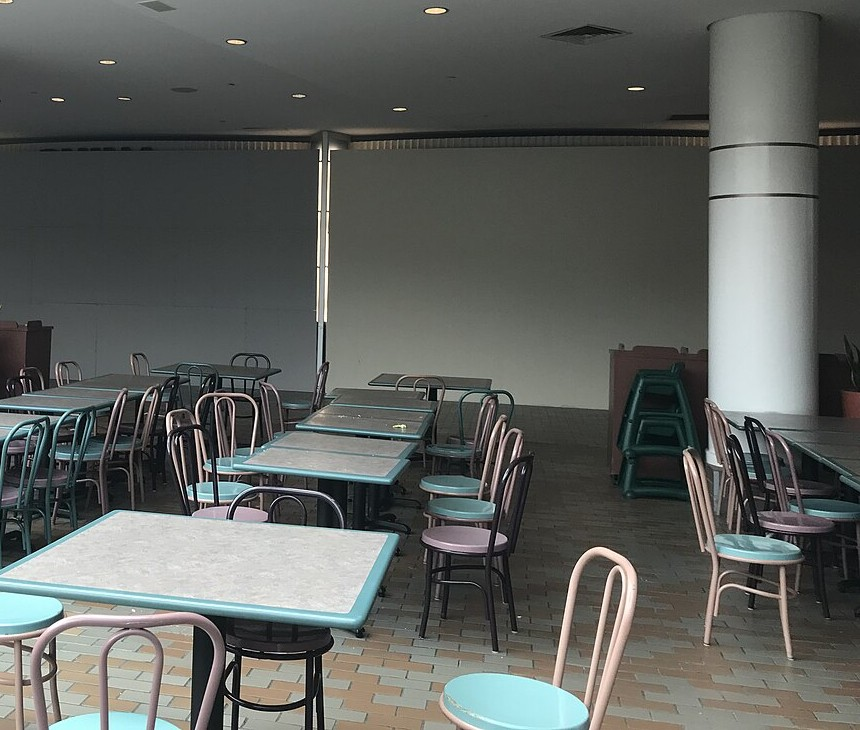
\includegraphics[width=0.45\textwidth]{images/web/empty_food_court_crop.jpg}
\caption[A food court]{A food court, whose tables are shared by everyone who wants to eat at the same time (photo by BornToZucc, cropped, \href{https://creativecommons.org/licenses/by-sa/4.0/}{CC~BY-SA~4.0}, via \href{https://commons.wikimedia.org/}{Wikimedia Commons}).}
\label{fig:intro-foodcourt}
\end{figure}

Several lines of research take this knowledge out of the person. CAROSA gives virtual characters roles, schedules and parameterized actions \citep{allbeck2010carosa}, and functional crowds follow roles and schedules in a building \citep{pelechano2008virtual}. Smart objects contain the information necessary to interact with them \citep{kallmann1999modeling}, characters in The Sims choose objects that advertise what they offer \citep{forbus2001notes}, and the Smart Objects of Unreal Engine let people reserve a slot \citep{epicgames2026smartobjects}. Menge breaks a crowd simulation down into components that can be swapped \citep{curtis2016menge}, and the ODD protocol asks modelers to report the entities and the scheduling of their model \citep{grimm2020odd}.

Our approach builds on these principles, so a person who studies a location should be able to specify the demand with explicit rules and state which resources the environment provides, without having to be a programmer. A new study should also leave the implementation of a person unchanged. Our central idea is that a stated time is a request, that is, a rule that defines when an activity may start, while the simulation decides when it actually starts.

\section{Main Goals}\label{sec:intro-goals}

The aim is to measure how shared resources affect the realized timetable of a place, so that a user can see where and why activities start later than authored. Authored rules, rather than code written for each individual case, give a population of boids purpose, a timetable and a range of activities, and the same system serves every study.

\subsection{Research question}\label{sub:intro-rq}

\begin{quote}
\emph{How can authored rules over capacity-limited stations, followed by a reusable population of boids, show where and why the realized timing of the activities in a place departs from the authored one?}
\end{quote}

The question has a measurement part and an authoring part. The measurement part asks what the recorded runs tell us about waiting, walking and capacity in each place, and the authoring part asks how few rule types and how little scenario code each study needs, as a reusable population keeps the class that represents a person, the movement layer and the resource model the same in every scenario. The scenarios test both parts, because they require routines, shared resources and emergencies to be written in the same way and then measured.

\subsection{Objectives}\label{sub:intro-objectives}

\Cref{chap:problem} sets out the functional requirements R1 to R7, and \cref{chap:conclusions} assesses each of the following objectives against them.

\begin{description}
\item[O1:] A language for purpose and timing, which is an \gls{xml} schedule format that states which person acts, when, with what action and on what target, with explicit rules for deferring, dispatching and dropping rules (R1, R2).
\item[O2:] A movement layer that takes each person to their target by combining navigation mesh path following with boids steering, while the environment, with its walking surfaces, walls, gates and exits, limits movement without being part of the rules (R5).
\item[O3:] Shared resources with a limited capacity, which are stations with places, a first-come, first-served queue and a service time, grouped into areas and used in ordered activities with several stages (R2, R3).
\item[O4:] Reuse across a range of scenarios, with several scenario families in \gls{ue} 5.4 built on a single implementation of a person, to find where reuse breaks down (R4).
\item[O5:] Measurement and a preliminary assessment, which use records of every rule, station visit and trip to show how capacity, travel and population affect the realized timing, and which measure how well the implementation scales on one machine (R6, R7).
\end{description}

\section{Document Structure}\label{sec:intro-structure}

Part~I contains this introduction, \cref{chap:soa} (\nameref{chap:soa}) and \cref{chap:problem} (\nameref{chap:problem}). \Cref{chap:soa} covers boids and steering, agent-based modeling, action selection and crowd models, and the work on purposeful populations, queueing, evacuation and validation. \Cref{chap:problem} describes the behavior we want, gives a high-level overview of our approach without technical detail, sets out the functional requirements R1 to R7 and discusses the difficulties in meeting them.

Part~II, the core of the dissertation, starts with \cref{chap:contribution}, which presents the framework first through the approach built during the pre-dissertation work and then through the architecture of the current pedestrian movement simulator. \Cref{chap:applications} evaluates the system on a daily urban routine, two shopping center layouts, an evacuation and a set of directed-flow corridors, and \cref{chap:conclusions} answers the research question and describes the future work. The appendices contain the per-run result tables (\cref{app:results}) and the build and analysis tooling (\cref{app:tooling}).

% State of the Art
\chapter{Boids, Agent-Based Models and Crowd Simulation}\label{chap:soa}

The chapter starts with boids, steering and the cost of neighbor search (\cref{sec:soa-boids}) and places boids within agent-based modeling (\cref{sec:ABM}). It then reviews action selection, the tools of the game engine and the crowd motion models (\cref{auto}), and it ends with the work on purposeful populations, queueing, evacuation and validation that is closest to this thesis, together with the gap that the thesis addresses (\cref{sec:soa-purpose,sec:soa-discussion}).

\section{Boids and Steering}\label{sec:soa-boids}

\citeauthor{reynolds1987flocks} introduced boids in \citeyear{reynolds1987flocks} as a distributed model for flocks, herds and schools (\cref{fig:soa-flocks}). Instead of following a global description, each boid senses its local surroundings and acts by a small number of local rules, and the behavior of the flock as a whole emerges from these local actions. \citet{vicsek1995novel} later showed that particles which only respond to their neighbors can move from disorder to order even in the presence of noise. We kept boids because the project started from a boid prototype (\cref{sec:first-impl}) and because they are easy to integrate into a game engine and have intuitive parameters, while the authoring layer of \cref{chap:contribution} does not depend on that choice.

\begin{figure}[H]
\centering
\begin{subfigure}[b]{0.40\textwidth}\centering
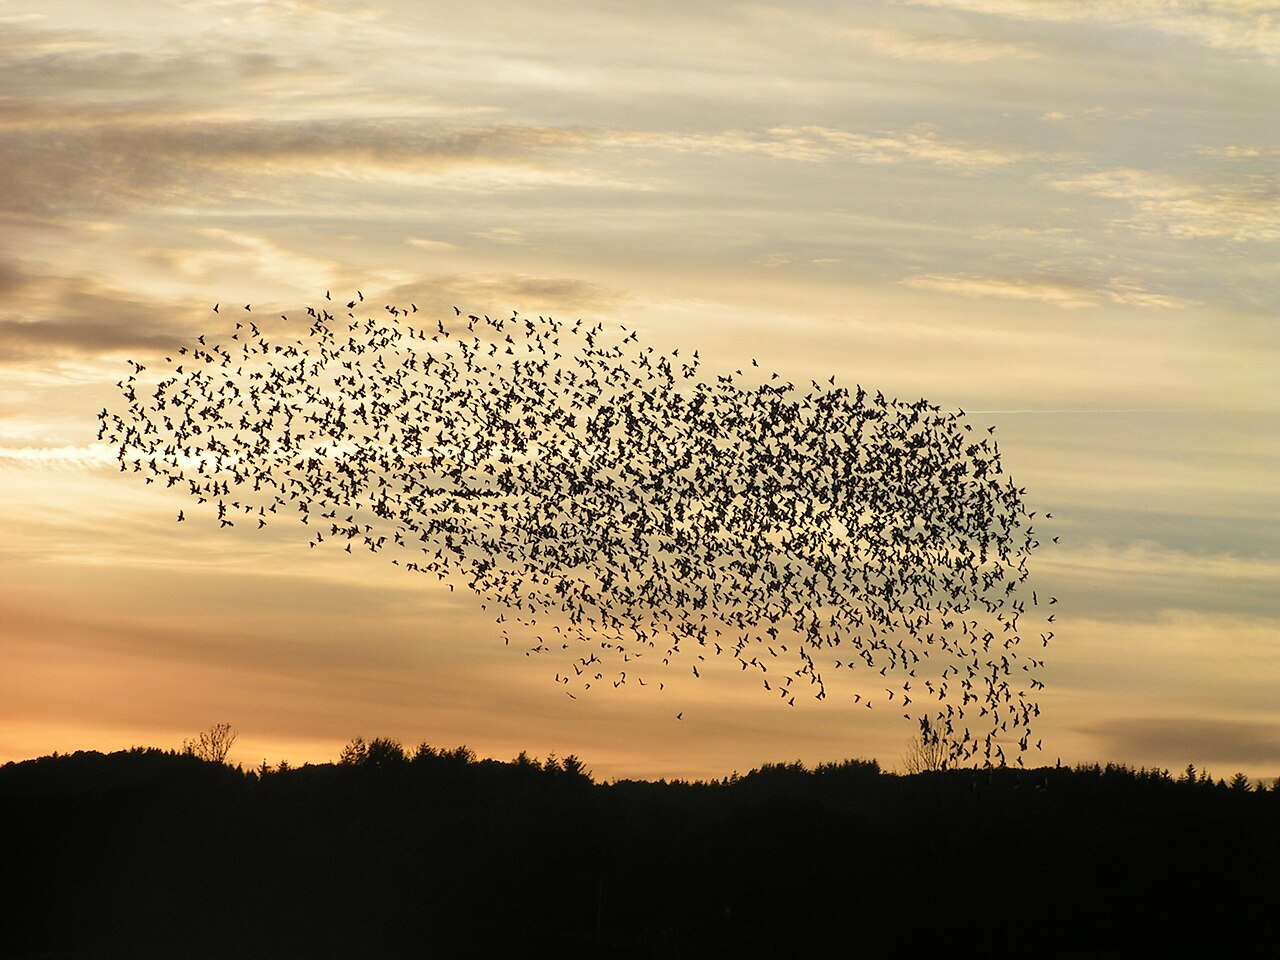
\includegraphics[width=\linewidth]{images/soa/murmuration.jpg}
\caption{Starlings over {\O}rns{\o}, Denmark}
\end{subfigure}\hspace{0.04\textwidth}
\begin{subfigure}[b]{0.40\textwidth}\centering
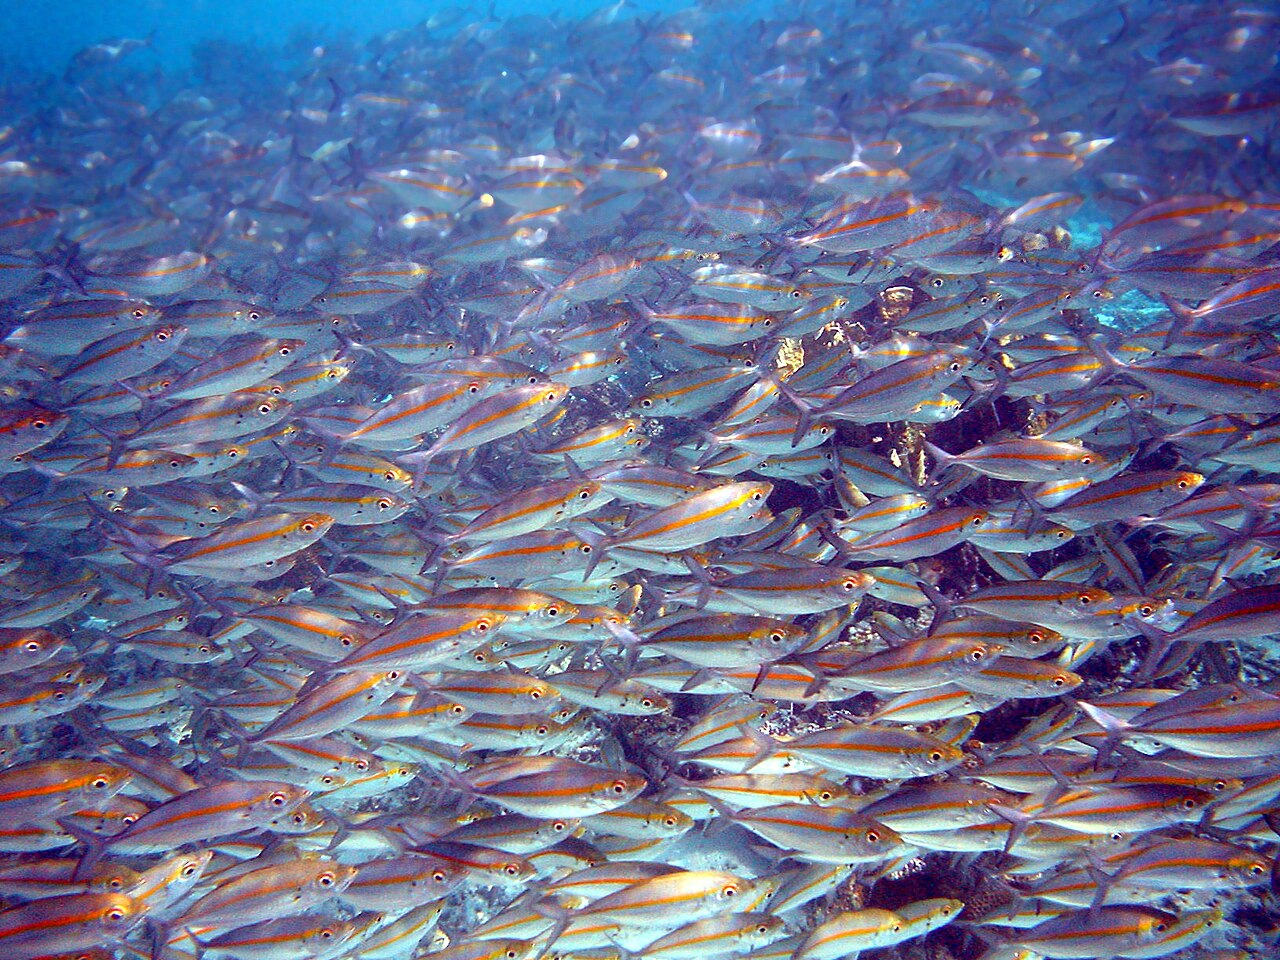
\includegraphics[width=\linewidth]{images/soa/fish_school.jpg}
\caption{A school of \emph{Pterocaesio chrysozona}}
\end{subfigure}
\caption[Collective motion in nature]{Collective motion in nature, with (a) starlings and (b) a fish school (photos by (a) Christoffer A. Rasmussen, public domain, and (b) Brocken Inaglory, \href{https://creativecommons.org/licenses/by-sa/3.0/}{CC~BY-SA~3.0}, via \href{https://commons.wikimedia.org/}{Wikimedia Commons}).}
\label{fig:soa-flocks}
\end{figure}

A boid is a vehicle that behaves as a point with a position $\mathbf{p}_i$ and a velocity $\mathbf{v}_i$, and it faces the direction of its velocity. At each update, it sees the set $N_i$ of flock members within a distance $r$ and a field of view $\theta$ measured from its direction of travel \citep{reynolds1987flocks}:
\begin{equation}
\boxed{N_i = \left\{\, j \neq i \;:\; \lVert \mathbf{p}_j - \mathbf{p}_i \rVert < r \;\wedge\; \angle\!\left(\mathbf{v}_i,\, \mathbf{p}_j - \mathbf{p}_i\right) < \tfrac{\theta}{2} \,\right\}}
\label{eq:neighbourhood}
\end{equation}
Three rules apply to this neighborhood, to avoid collision, to match velocity and to stay close (\cref{fig:boids-rules}). Reynolds expressed them in words, and the equations below are a typical way of writing them, each giving zero when $N_i$ is empty. Separation sums the vectors that point away from each neighbor, weighted by the inverse square of the distance, alignment matches the mean velocity of the neighbors, and cohesion pulls the boid toward their centroid:
\begin{equation}
\boxed{\mathbf{s}_i = \sum_{j \in N_i} \frac{\mathbf{p}_i - \mathbf{p}_j}{\lVert \mathbf{p}_i - \mathbf{p}_j \rVert^{2}}}
\label{eq:separation}
\end{equation}
\begin{equation}
\boxed{\mathbf{a}_i = \frac{1}{\lvert N_i \rvert} \sum_{j \in N_i} \mathbf{v}_j \;-\; \mathbf{v}_i}
\label{eq:alignment}
\end{equation}
\begin{equation}
\boxed{\mathbf{c}_i = \frac{1}{\lvert N_i \rvert} \sum_{j \in N_i} \mathbf{p}_j \;-\; \mathbf{p}_i}
\label{eq:cohesion}
\end{equation}
Separation is the only rule that keeps boids apart, and it is a weak constraint, because proximity only has a cost and boids can still overlap when other forces dominate. The centroid is local, so a flock can split around an obstacle and rejoin. Strangers on a street have no reason to stay together, so for pedestrians cohesion is generally low, present only within a group, and overridden by each person's destination.

\begin{figure}[H]
\centering
\begin{subfigure}[b]{0.31\textwidth}\centering
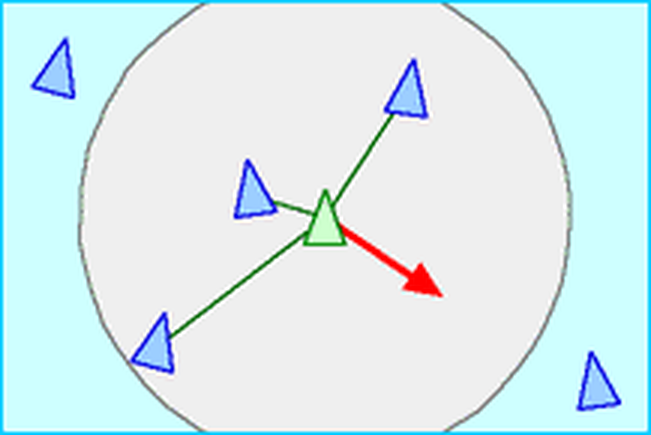
\includegraphics[width=\linewidth]{images/web/boids_rule_separation.png}
\caption{Separation}
\end{subfigure}\hfill
\begin{subfigure}[b]{0.31\textwidth}\centering
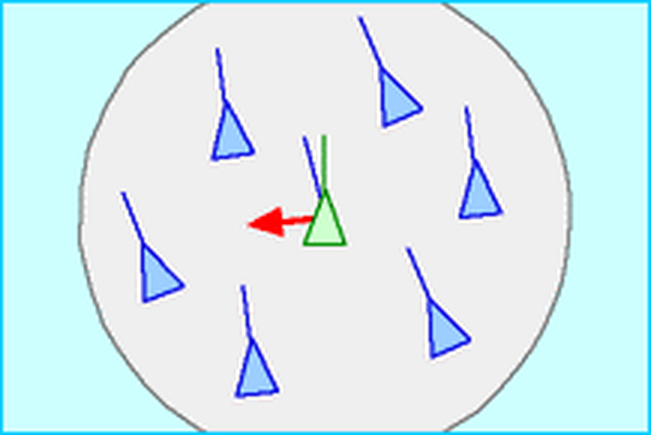
\includegraphics[width=\linewidth]{images/web/boids_rule_alignment.png}
\caption{Alignment}
\end{subfigure}\hfill
\begin{subfigure}[b]{0.31\textwidth}\centering
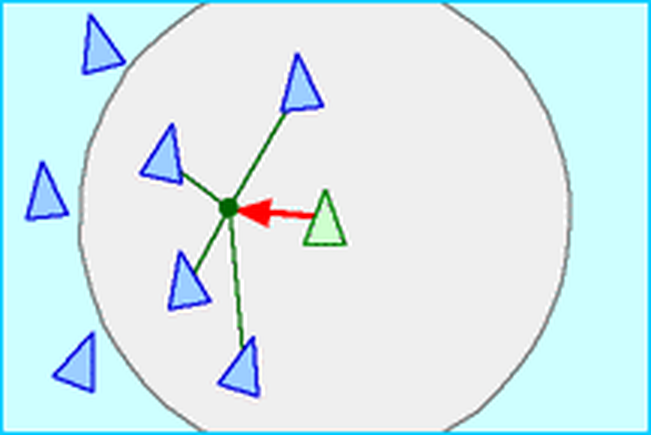
\includegraphics[width=\linewidth]{images/web/boids_rule_cohesion.png}
\caption{Cohesion}
\end{subfigure}
\caption[The three boids rules]{The three boids rules seen from the green boid, where the grey disc is its neighborhood and the red arrow is the steering that each rule produces (diagrams by Craig Reynolds, public domain, via \href{https://commons.wikimedia.org/}{Wikimedia Commons}).}
\label{fig:boids-rules}
\end{figure}

\citet{reynolds1999steering} built a library of steering behaviors on these rules and split movement into \emph{action selection} (choosing a goal), \emph{steering} (turning the goal into a desired change in motion) and \emph{locomotion} (the movement itself, \cref{fig:steering-pipeline}). In our design, authored rules take care of action selection and the boids-based navigation takes care of steering. The vehicle is a point mass $m$ with a maximum force $f_{\max}$ and a maximum speed $v_{\max}$:
\begin{equation}
\boxed{\mathbf{v} \leftarrow \operatorname{trunc}\!\left(\mathbf{v} + \frac{\operatorname{trunc}(\mathbf{f}, f_{\max})}{m}\,\Delta t,\; v_{\max}\right)\qquad
\mathbf{p} \leftarrow \mathbf{p} + \mathbf{v}\,\Delta t}
\label{eq:vehicle}
\end{equation}
Most behaviors compute a desired velocity $\mathbf{v}^{d}$ and set $\mathbf{f}$ to $\mathbf{v}^{d}$ minus $\mathbf{v}$, as in seek and flee, arrival, pursuit and evasion, wander, path following, obstacle avoidance with probes in front of the individual, and leader following.

\begin{figure}[H]
\centering
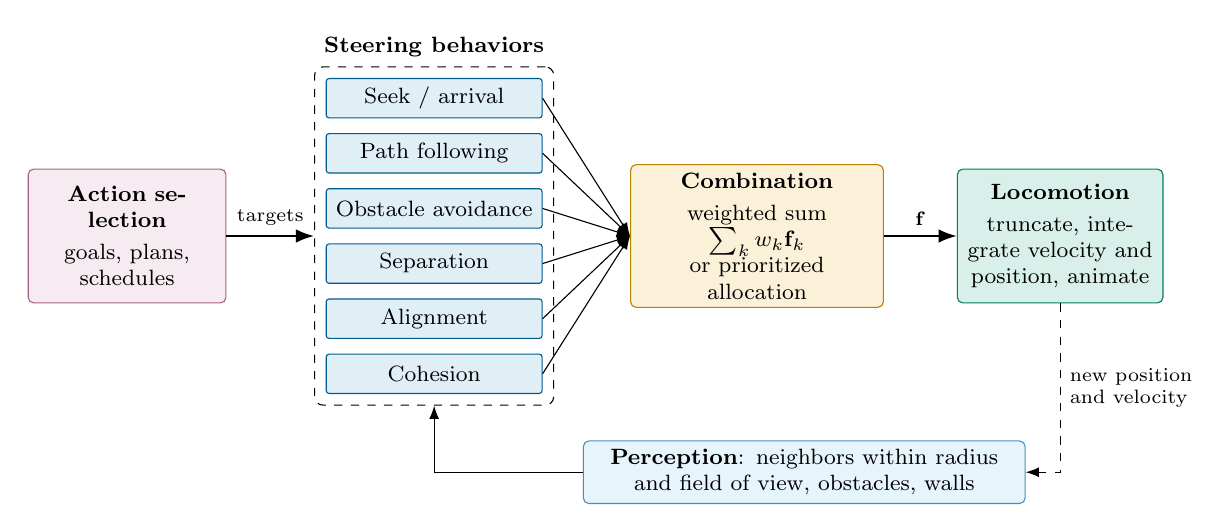
\begin{tikzpicture}[>=Latex, font=\footnotesize,
  box/.style={draw,rounded corners=2pt,align=center,inner sep=3pt},
  beh/.style={draw=cBlue!80!black,rounded corners=1pt,align=center,text width=2.6cm,minimum height=0.5cm,inner sep=2pt,fill=cBlue!12}]
\node[box,text width=2.3cm,minimum height=1.7cm,fill=cPurple!15,draw=cPurple!80!black] (sel) at (0,0) {\textbf{Action selection}\\[2pt]goals, plans, schedules};
\node[beh] (b1) at (3.9,1.75) {Seek / arrival};
\node[beh] (b2) at (3.9,1.05) {Path following};
\node[beh] (b3) at (3.9,0.35) {Obstacle avoidance};
\node[beh] (b4) at (3.9,-0.35) {Separation};
\node[beh] (b5) at (3.9,-1.05) {Alignment};
\node[beh] (b6) at (3.9,-1.75) {Cohesion};
\node[draw,dashed,rounded corners=3pt,fit=(b1)(b6),inner sep=4pt,label={[font=\footnotesize\bfseries]above:Steering behaviors}] (steer) {};
\node[box,text width=3.0cm,minimum height=1.7cm,fill=cOrange!15,draw=cOrange!80!black] (comb) at (8.0,0) {\textbf{Combination}\\[2pt]weighted sum $\sum_k w_k \mathbf{f}_k$\\or prioritized allocation};
\node[box,text width=2.4cm,minimum height=1.7cm,fill=cGreen!15,draw=cGreen!80!black] (loc) at (11.85,0) {\textbf{Locomotion}\\[2pt]truncate, integrate velocity and position, animate};
\node[box,text width=5.4cm,fill=cSky!15,draw=cSky!80!black] (per) at (8.6,-3.0) {\textbf{Perception}: neighbors within radius and field of view, obstacles, walls};
\draw[->,thick] (sel.east) -- node[above,font=\scriptsize]{targets} (sel.east -| steer.west);
\foreach \b in {b1,b2,b3,b4,b5,b6} \draw[->] (\b.east) -- (comb.west);
\draw[->,thick] (comb) -- node[above,font=\scriptsize]{$\mathbf{f}$} (loc);
\draw[->] (per.west) -| (steer.south);
\draw[->,dashed] (loc.south) |- node[pos=0.25,right,font=\scriptsize,align=left]{new position\\and velocity} (per.east);
\end{tikzpicture}
\caption[Steering between action selection and locomotion]{Steering behaviors between action selection and locomotion, after \citet{reynolds1999steering}.}
\label{fig:steering-pipeline}
\end{figure}

\subsection{Combining Behaviors}\label{combo}

A pedestrian that follows a path must also keep clear of other pedestrians and of walls, and the weighted sum is the simplest way of combining the forces, as \citet{reynolds1999steering} noted:
\begin{equation}
\boxed{\mathbf{f} = \operatorname{trunc}\!\left(\sum_{k} w_k\,\mathbf{f}_k,\; f_{\max}\right)}
\label{eq:weighted}
\end{equation}
It is cheap and gives smooth motion, but opposing forces can cancel each other out and leave the character stuck, a small force can hide a larger one, and weights that work in one situation may fail in another \citep{millington2019ai}. The alternative is priority, as in Reynolds' prioritized acceleration allocation, where requests fill an accumulator in order of priority until it reaches its capacity, and textbooks also blend within priority groups \citep{millington2019ai}. Many systems, ours included, use priority between layers and blending within a layer. Extensions of the original rules add forces for leadership changes \citep{hartman2006autonomous}, fear signals that reach animals which cannot see the threat \citep{delgadomata2007fear} and escape, which in a building means competing for exits, where pushing makes everyone slower \citep{helbing2000simulating}.

\subsection{Cost of Neighbor Search}\label{sub:complexity}

In each frame, each boid evaluates \cref{eq:neighbourhood,eq:separation,eq:alignment,eq:cohesion} from a snapshot of the previous state, combines the forces with \cref{eq:weighted} and integrates them with \cref{eq:vehicle}, so the result does not depend on the order of updates and the algorithm parallelizes well. A direct search performs $O(n^2)$ distance tests per frame, which is the main bottleneck with thousands of individuals. The usual remedy is a uniform grid whose cells are at least as large as the perception radius, so that a query visits only the neighboring cells and its cost depends on the local density \citep{ericson2004realtime,reynolds2006big}. Hierarchical structures such as k-d trees \citep{bentley1975multidimensional} adapt better to clustered individuals but cost more to rebuild every frame (\cref{fig:soa-kdtree}). General-purpose \gls{gpu} computation suits boids, because each individual only reads the previous state \citep{owens2007survey,joselli2009neighborhood}, and approximate or capped neighbor sets reduce the cost further \citep{joselli2009neighborhood,silva2009boids}, although these change the model and should be reported.

\begin{figure}[H]
\centering
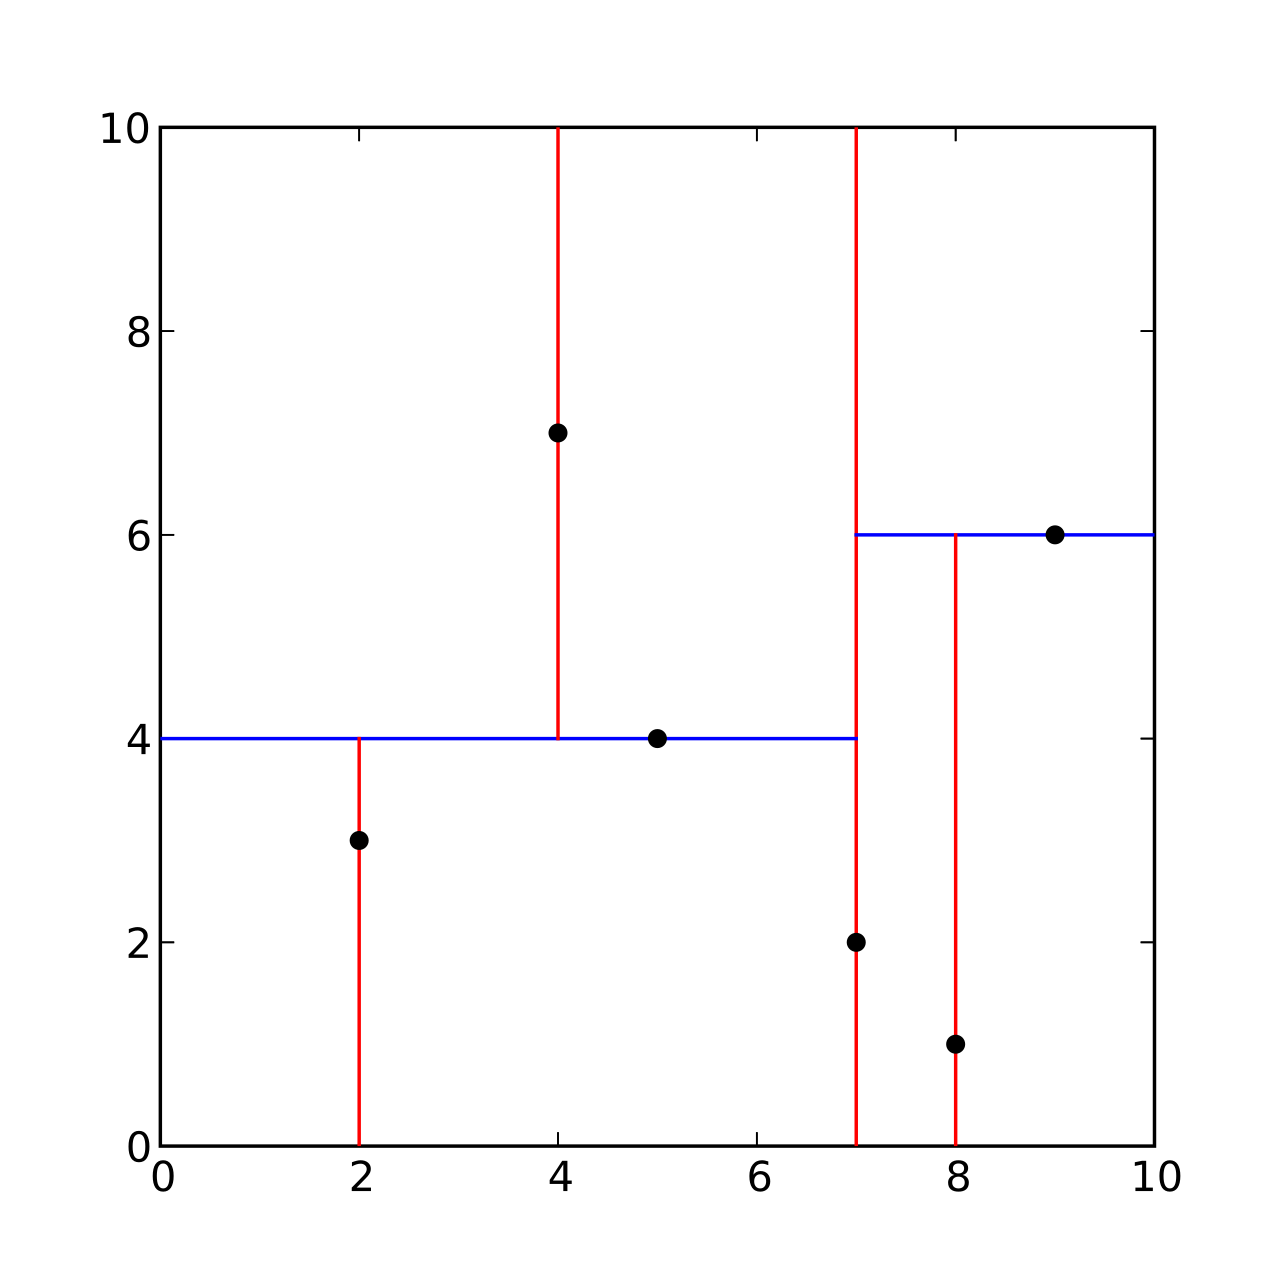
\includegraphics[width=0.30\textwidth]{images/soa/kdtree.png}
\caption[A two-dimensional k-d tree]{A two-dimensional k-d tree for seven points (image by KiwiSunset, English Wikipedia, \href{https://creativecommons.org/licenses/by-sa/3.0/}{CC~BY-SA~3.0}, via \href{https://commons.wikimedia.org/}{Wikimedia Commons}).}
\label{fig:soa-kdtree}
\end{figure}

\section{Agent-Based Modeling}\label{sec:ABM}

An \gls{abm} represents a system as a collection of autonomous individuals, each of which assesses its own situation and acts according to a set of rules \citep{bonabeau2002agent}, and boids are a classic example. \citet{macal2010tutorial} describe a model through individuals with attributes and behaviors, their interactions and their environment. Toolkits such as NetLogo \citep{wilensky1999netlogo}, MASON \citep{luke2005mason} and Repast Simphony \citep{north2013complex} target general modeling rather than animated characters on navigation meshes, which is one reason why interactive crowds are built inside game engines. Outcomes are usually emergent, as with lane formation in counter-flows \citep{helbing2005self}, so modelers observe them over many seeded runs and summarize them statistically. The \acrshort{odd} protocol \citep{grimm2006standard,grimm2020odd} also asks modelers to report hidden design decisions, such as the order of updates and how time advances.

A population can be studied top-down through aggregate equations, as when \citet{hughes2002continuum} treats the crowd as a fluid moving down a potential, or bottom-up through individuals. \citet{vandykeparunak1998agent} found that agent-based models suit systems with discrete decision makers, each with its own history, while equation-based models suit systems that aggregates describe well. Corridor flow obeys aggregate relations, but whether a worker finds a free desk depends on what other people did that morning, which is the kind of question this thesis addresses.

\section{Action Selection and Crowd Models}\label{auto}

A \gls{fsm} has one state at a time and changes state when a condition is met, so the number of transitions grows quickly as states are added \citep{millington2019ai}. Behavior trees, popularized by Halo~2 \citep{isla2005handling}, compose sequences and selectors from leaves and are more modular and reactive \citep{millington2019ai,colledanchise2018behavior} (\cref{fig:soa-bt}). Goal-oriented action planning searches for actions whose preconditions and effects reach a goal \citep{orkin2006three}, and utility-based selection scores the options \citep{graham2019introduction}. These describe how to behave rather than when, so time of day and resource availability must be modeled separately. Other work moves knowledge into the environment, with smart objects that describe how they are used \citep{kallmann1999modeling}, objects in The Sims that advertise how much they satisfy a motivation \citep{forbus2001notes} and behaviors attached to regions \citep{sung2004scalable}, and our stations derive from these ideas. Data-driven and learned approaches reuse recorded trajectories \citep{lerner2007crowds} or train individual policies \citep{juliani2018unity}, such as collision avoidance \citep{lee2018crowd}, but they address local motion, and a user who must state who arrives when gains little from a policy that hides its assumptions in weights.

\begin{figure}[H]
\centering
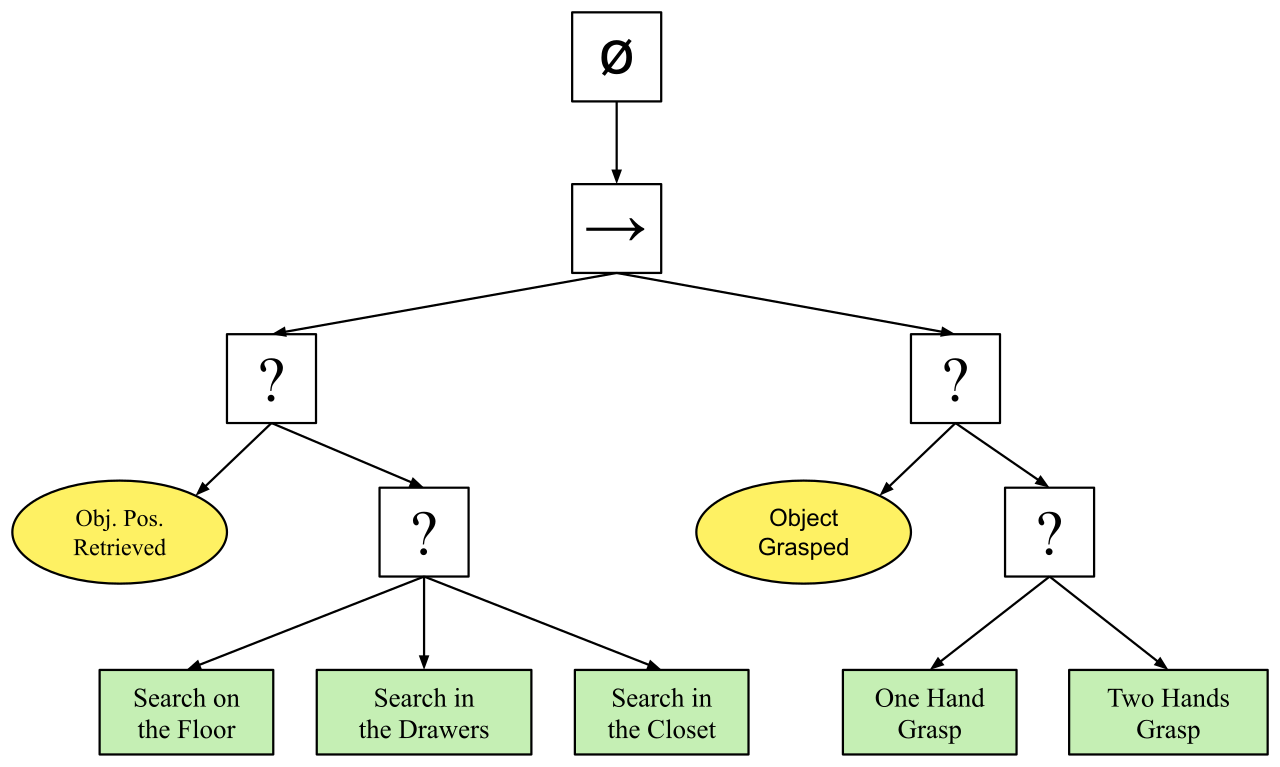
\includegraphics[width=0.45\textwidth]{images/soa/behaviour_tree.png}
\caption[A behavior tree]{A behavior tree for a robot that finds and grasps an object \citep{colledanchise2018behavior} (diagram by Aliekor, English Wikipedia, \href{https://creativecommons.org/licenses/by-sa/3.0/}{CC~BY-SA~3.0}, via \href{https://commons.wikimedia.org/}{Wikimedia Commons}).}
\label{fig:soa-bt}
\end{figure}

Game engines now provide much of this infrastructure, and we draw on the current Unreal Engine documentation for its concepts, although the implementation uses version~5.4. The Navigation System builds a navigation mesh with Recast and answers path queries \citep{epicgames2026navigation,mononen2009recast} (\cref{fig:soa-navmesh}), with \gls{rvo} avoidance in the Character Movement component and adaptive \gls{rvo} sampling in the Detour Crowd manager \citep{epicgames2026avoidance}. Behavior trees and State Trees support decisions \citep{epicgames2026statetree}, Smart Objects have slots that characters claim and release \citep{epicgames2026smartobjects}, and Mass Entity, the Mass Gameplay plugins and ZoneGraph lanes support large numbers of characters \citep{epicgames2026massentity,epicgames2026massgameplay,epicgames2026zonegraph}. Who does what and when, the order of waiting and the service time are all left to the developer. Unlike Smart Objects, which let characters claim and release slots, our stations add a capacity, a first-come, first-served queue, a timed service and ordered multi-stage use, and our schedules add the timing and deferral rules that decide when each request is made. Menge makes goal selection, planning and local avoidance pluggable components \citep{curtis2016menge}, which is also our motivation at the boundary between activity and movement.

\begin{figure}[H]
\centering
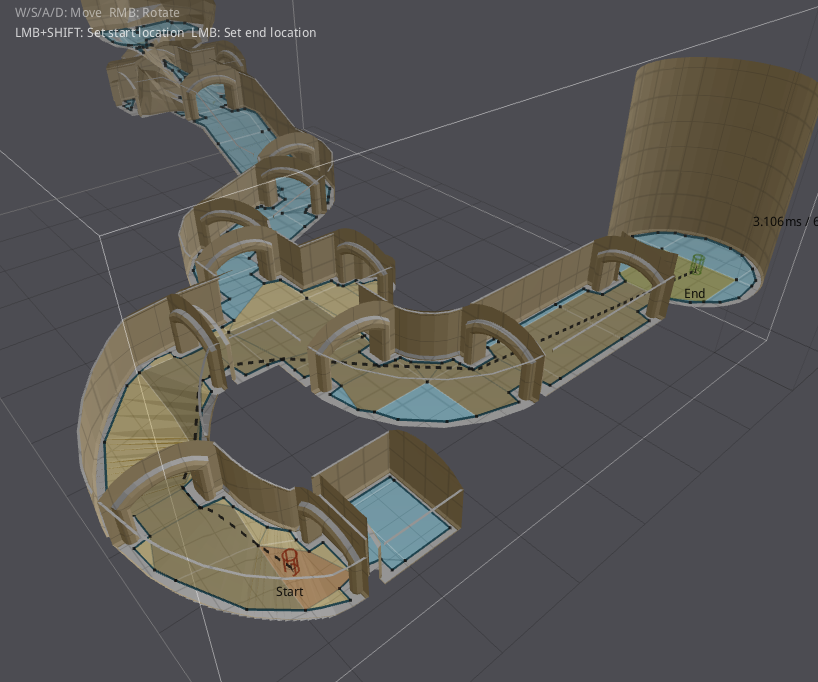
\includegraphics[width=0.42\textwidth]{images/soa/recast_navmesh_crop.png}
\caption[A navigation mesh built by Recast]{A navigation mesh built by Recast, with a path found by Detour (cropped screenshot of RecastDemo, Recast \& Detour \textcopyright{}~2009 Mikko Mononen, zlib license, \href{https://github.com/recastnavigation/recastnavigation}{github.com/recastnavigation}).}
\label{fig:soa-navmesh}
\end{figure}

General references on crowd simulation are \citet{thalmann2013crowd}, \citet{pelechano2008virtual} and \citet{kapadia2016virtual}, with a history by \citet{musse2021history}, and the motion models below all take their targets from an action selection layer (\cref{fig:model-taxonomy}). Macroscopic models evolve a density field over a cost potential \citep{hughes2002continuum,treuille2006continuum}, and cellular automata with floor fields \citep{burstedde2001simulation,kirchner2002simulation} are fast but too coarse for animated motion (\cref{fig:soa-ca}). Microscopic models compute motion per pedestrian with social forces \citep{helbing1995social}, HiDAC \mbox{\citep{pelechano2007controlling}}, reciprocal velocity obstacles and \gls{orca} \citep{vandenberg2008reciprocal,vandenberg2011reciprocal} (\cref{fig:soa-vo}), a time-to-collision law \citep{karamouzas2014universal} or vision-based heuristics \citep{moussaid2011simple}, as surveyed by \citet{vantoll2021algorithms}. Force-based models and boids only penalize overlap, velocity obstacle models avoid it under their own assumptions, and the walker experiments of \citet{pettre2009experiment} show that both people share the avoidance. None of these models provides targets, so the authoring problem would be the same with any of them.

\begin{figure}[H]
\centering
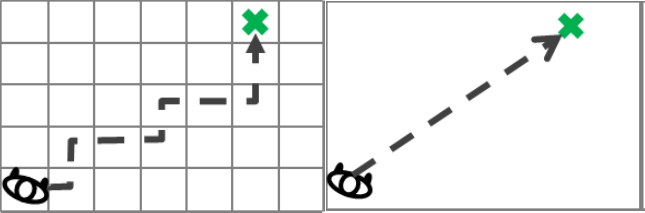
\includegraphics[width=0.5\textwidth]{images/soa/grid_vs_continuous.png}
\caption[Movement on a grid and in continuous space]{Movement on a grid of cells, on the left, and in continuous space, on the right (diagram by Angelika Kneidl, \href{https://creativecommons.org/licenses/by-sa/4.0/}{CC~BY-SA~4.0}, via \href{https://commons.wikimedia.org/}{Wikimedia Commons}).}
\label{fig:soa-ca}
\end{figure}

\begin{figure}[H]
\centering
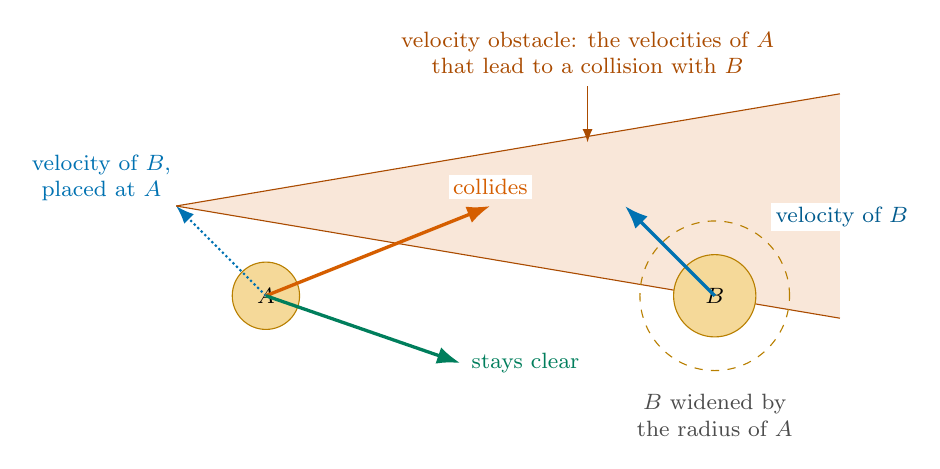
\begin{tikzpicture}[>=Latex, font=\footnotesize, scale=0.95,
  lab/.style={fill=white,inner sep=1.5pt,align=center}]
% cone of velocities of A that hit B: apex at A + v_B, edges parallel to the tangents from A to the widened B
\fill[cVerm!15] (-1.2,1.2) -- (7.674,2.7) -- (7.674,-0.3) -- cycle;
\draw[cVerm!80!black] (-1.2,1.2) -- (7.674,2.7);
\draw[cVerm!80!black] (-1.2,1.2) -- (7.674,-0.3);
% the two people
\draw[cOrange!80!black,dashed] (6,0) circle (1.0);
\filldraw[fill=cOrange!40,draw=cOrange!80!black] (0,0) circle (0.45) node {$A$};
\filldraw[fill=cOrange!40,draw=cOrange!80!black] (6,0) circle (0.55) node {$B$};
\node[lab,text=black!70] at (6,-1.6) {$B$ widened by\\the radius of $A$};
% B's velocity, and the same vector placed at A, which moves the apex of the cone
\draw[->,very thick,cBlue] (6,0) -- (4.8,1.2);
\node[lab,text=cBlue!80!black,anchor=west] at (6.75,1.05) {velocity of $B$};
\draw[->,thick,cBlue,densely dotted] (0,0) -- (-1.2,1.2) node[lab,above left=0pt]{velocity of $B$,\\placed at $A$};
% two candidate velocities of A
\draw[->,very thick,cVerm] (0,0) -- (3.0,1.2) node[lab,above=2pt]{collides};
\draw[->,very thick,cGreen!80!black] (0,0) -- (2.6,-0.9) node[lab,right=2pt]{stays clear};
\node[lab,text=cVerm!80!black] at (4.3,3.25) {velocity obstacle: the velocities of $A$\\that lead to a collision with $B$};
\draw[->,cVerm!80!black] (4.3,2.8) -- (4.3,2.05);
\end{tikzpicture}
\caption[A velocity obstacle]{A velocity obstacle, where every velocity of $A$ that ends inside the shaded cone leads to a collision with $B$ if both keep moving, so velocity obstacle models choose a velocity outside it \citep{vandenberg2008reciprocal}.}
\label{fig:soa-vo}
\end{figure}

\begin{figure}[H]
\centering
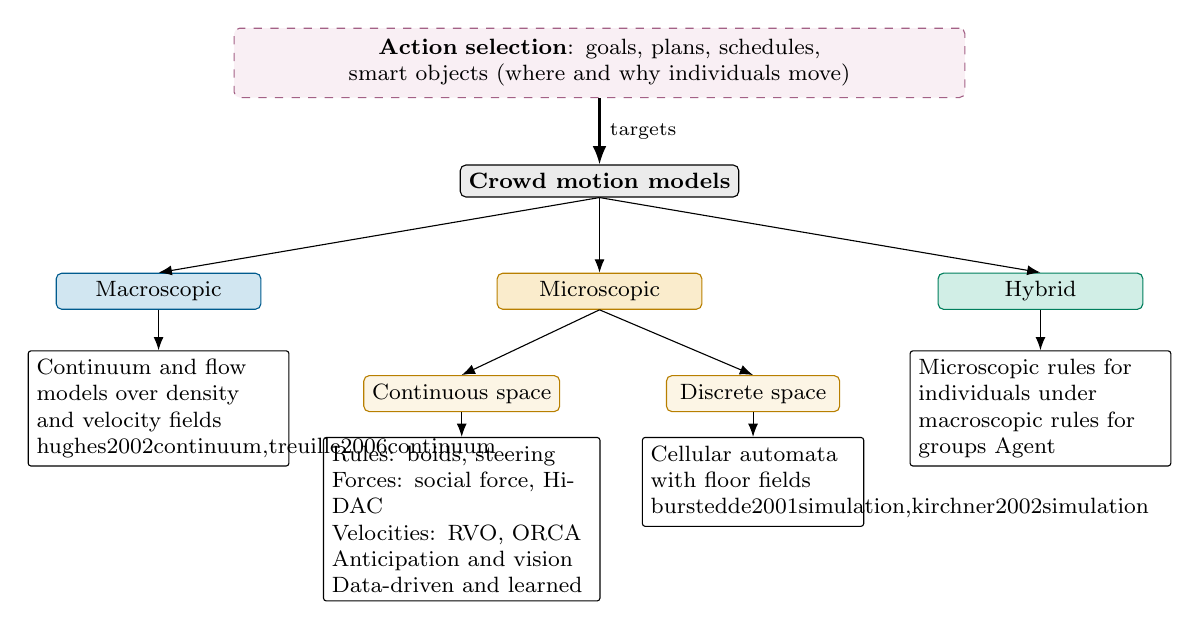
\begin{tikzpicture}[>=Latex, font=\footnotesize,
  cat/.style={draw,rounded corners=2pt,align=center,inner sep=3pt,fill=black!8,minimum width=2.6cm},
  leaf/.style={draw,rounded corners=1pt,align=left,inner sep=3pt},
  edge/.style={->}]
\node[draw=cPurple!80!black,dashed,rounded corners=2pt,align=center,text width=9cm,inner sep=4pt,fill=cPurple!12] (sel) at (0,1.5) {\textbf{Action selection}: goals, plans, schedules, smart objects (where and why individuals move)};
\node[cat] (root) at (0,0) {\textbf{Crowd motion models}};
\draw[edge,thick] (sel) -- node[right,font=\scriptsize]{targets} (root);
\node[cat,fill=cBlue!18,draw=cBlue!80!black] (macro) at (-5.6,-1.4) {Macroscopic};
\node[cat,fill=cOrange!20,draw=cOrange!80!black] (micro) at (0,-1.4) {Microscopic};
\node[cat,fill=cGreen!18,draw=cGreen!80!black] (hyb) at (5.6,-1.4) {Hybrid};
\draw[edge] (root.south) -- (macro.north);
\draw[edge] (root.south) -- (micro.north);
\draw[edge] (root.south) -- (hyb.north);
\node[cat,minimum width=2.2cm,fill=cOrange!10,draw=cOrange!80!black] (cont) at (-1.75,-2.7) {Continuous space};
\node[cat,minimum width=2.2cm,fill=cOrange!10,draw=cOrange!80!black] (disc) at (1.95,-2.7) {Discrete space};
\draw[edge] (micro.south) -- (cont.north);
\draw[edge] (micro.south) -- (disc.north);
\node[leaf,text width=3.1cm,anchor=north] (macroleaf) at (-5.6,-2.15) {Continuum and flow models over density and velocity fields \citep{hughes2002continuum,treuille2006continuum}};
\node[leaf,text width=3.3cm,anchor=north] (contleaf) at (-1.75,-3.25) {Rules: boids, steering\\Forces: social force, HiDAC\\Velocities: RVO, ORCA\\Anticipation and vision\\Data-driven and learned};
\node[leaf,text width=2.6cm,anchor=north] (discleaf) at (1.95,-3.25) {Cellular automata with floor fields \citep{burstedde2001simulation,kirchner2002simulation}};
\node[leaf,text width=3.1cm,anchor=north] (hybleaf) at (5.6,-2.15) {Microscopic rules for individuals under macroscopic rules for groups \citep{Agent}};
\draw[edge] (macro) -- (macroleaf);
\draw[edge] (cont) -- (contleaf);
\draw[edge] (disc) -- (discleaf);
\draw[edge] (hyb) -- (hybleaf);
\end{tikzpicture}
\caption[A taxonomy of crowd motion models]{A taxonomy of crowd motion models.}
\label{fig:model-taxonomy}
\end{figure}

\section{Purposeful Populations and Shared Resources}\label{sec:soa-purpose}

Systems that aim for believable populations combine decision-making with crowd motion, usually in layers. \citet{hoogendoorn2004pedestrian} distinguish a strategic level (choosing and scheduling activities), a tactical level (areas and routes) and an operational level (walking), and \citet{musse2001hierarchical} and Menge \citep{curtis2016menge} layer control in a similar way. In our system, schedules and stations act at the strategic and tactical levels and the boid-guided paths at the operational level.

Several systems give a population purpose through activities: needs-driven travelers in Pennsylvania Station \citep{shao2007autonomous}, an activity-driven population \citep{paris2009activity}, roles and schedules \citep{pelechano2008virtual}, CAROSA's roles, schedules and parameterized actions \citep{allbeck2010carosa}, transit trips generated for a crowd simulator \citep{ricks2020generation} and MATSim's daily activity plans, which are improved through repeated simulation \citep{horni2016matsim}, and \cref{tab:activity-systems} compares them with this thesis. Authored time-of-day schedules are also common in commercial games, as role-playing games such as The Elder Scrolls IV: Oblivion \citep{bethesda2006oblivion} and V: Skyrim \citep{bethesda2011skyrim} give their non-player characters daily packages with time windows. Farming games such as Stardew Valley \citep{concernedape2016stardew} read the schedules of their characters from data files. Pedestrian simulators for building design, such as MassMotion \citep{oasys2026massmotion}, Pathfinder \citep{thunderhead2026pathfinder}, Vadere \citep{kleinmeier2019vadere} and JuPedSim \citep{jupedsim2026}, model services, waiting areas and queues. Neither group combines authored schedules with capacity-limited resources and boids steering inside a general game engine, but both show that schedules and queues on their own are not new, so our contribution lies in their combination and in the timing semantics of \cref{chap:problem}.

\citet{Agent}\label{sec:soa-saeed} combine microscopic rules for pedestrians, who have attributes such as age, velocity and energy, with macroscopic rules for subgroups that share an intention over several goal points. They sum the steering, obstacle and pedestrian-avoidance forces into one, combine flocking with pathfinding over a navigation mesh \citep{hart1968formal,snook2000simplified} and first test their components in a simple scenario, as the scenario suites of SteerBench \citep{singh2009steerbench} and RiMEA \citep{rimea2025guideline} also do. It is the published work closest to our movement design, while \citet{shao2007autonomous} and CAROSA \citep{allbeck2010carosa} are closer on timing and resources. As we read it, it addresses motion, with goals and group intentions but no timed schedules or capacity constraints. In their summed forces the flock can pull individuals off their route, while in our hybrid boids the path dominates and steering can only turn the heading by a bounded amount.

\begin{table}[H]
\centering
\footnotesize
\begin{tabularx}{\textwidth}{|>{\raggedright\arraybackslash}p{2.5cm}|>{\raggedright\arraybackslash}X|>{\raggedright\arraybackslash}X|>{\raggedright\arraybackslash}X|>{\raggedright\arraybackslash}X|}
\hline
\rowcolor{headgray}\textbf{Work} & \textbf{Source of purpose} & \textbf{Timing of activities} & \textbf{Shared resources} & \textbf{Local motion} \\
\hline
\citet{shao2007autonomous} & Internal needs and goals in a cognitive layer & Driven by needs and events & Ticket queues in the station & Reactive behaviors with perception \\ \hline
\citet{paris2009activity} & Cognitive, goal-oriented activities & Activity-driven & Not a focus & Not a focus \\ \hline
CAROSA \citep{allbeck2010carosa} & Roles and parameterized actions & Authored schedules & Not a focus & Not a focus \\ \hline
\citet{ricks2020generation} & Generated trips in a transit facility & Generated arrival and destination times & Not a focus & Separate crowd simulator \\ \hline
MATSim \citep{horni2016matsim} & Daily activity plans & Activity times in plans, improved by replanning & Not at pedestrian level & Network-level trips, no steering \\ \hline
Menge \citep{curtis2016menge} & Finite-state goal selection & Not a focus & Not a focus & Replaceable local-avoidance component \\ \hline
Unreal Engine tools \citep{epicgames2026statetree,epicgames2026smartobjects} & Behavior trees or State Tree written by the developer & Developer's own logic & Smart Object slots claimed and released & Navigation mesh paths with avoidance \\ \hline
\citet{Agent} & Group intentions over several goal points & Not a focus & Not a focus & Combined steering forces \\ \hline
This thesis & Authored timed rules in readable files & Rules eligible from a time, deferred while the person is busy & Stations with capacity, \glsentryshort{fifo} queue and service time & Boids bounded around navigation mesh paths \\ \hline
\end{tabularx}
\caption[Systems that give simulated populations purpose]{Systems that give simulated populations purpose, where ``not a focus'' means that the work does not present that aspect.}
\label{tab:activity-systems}
\end{table}

Once individuals need resources, waiting is part of the outcome. In Kendall's notation, a counter with $c$ places is an M/M/$c$ or, without statistical assumptions, a G/G/$c$ queue \citep{kendall1953stochastic}. Little's law ($L = \lambda W$) links the mean number in a system to the arrival rate and the mean time spent in it \citep{little1961proof}, and waiting grows sharply as the utilization $\rho = \lambda/(c\mu)$ approaches 1 \citep{shortle2018fundamentals}. These results assume steady arrivals, but scheduled demand comes in waves and late starts push later arrivals, so we measure queues rather than calculate them, as discrete-event simulation does \citep{law2015simulation}. Commercial pedestrian tools such as the AnyLogic Pedestrian Library combine walking with services, waiting areas and queues \citep{anylogic2026pedestrian}, but they model a facility, while our setting is a game-engine population with authored schedules. Physical space is a second dimension, as Fruin's levels of service rate areas by space per pedestrian \citep{fruin1971pedestrian}, Weidmann relates walking speed (about 1.34~m/s when free) to density \citep{weidmann1993transporttechnik} and HiDAC models queueing physically \mbox{\citep{pelechano2007controlling}}. A queue kept as an ordered list ignores these effects, which makes timing analysis much easier but limits the claims that can be made about crowding.

For a purposeful crowd, evacuation and validation remain open. \citet{schadschneider2009evacuation} review evacuation research, whose simulations reproduce clogging and the faster-is-slower effect \citep{helbing2000simulating}, and \citet{kuligowski2010review} compare the models in use. In an activity-driven population, individuals are queueing, being served or walking when the alarm sounds, and where they were shapes how they leave. Validation compares a simulation with real behavior, through fundamental diagrams for single files \citep{seyfried2005fundamental} and for corridors and T-junctions \citep{zhang2011transitions}, pairwise avoidance against motion capture \citep{pettre2009experiment}, stop-and-go waves \citep{lemercier2012realistic}, lane formation and bottleneck oscillations \citep{helbing2005self}, and experiments in which people steer avatars in a virtual environment \citep{moussaid2016crowd} (\cref{fig:soa-bottleneck}). SteerBench \citep{singh2009steerbench}, the RiMEA test cases \citep{rimea2025guideline} and ISO~20414 \citep{iso2020evacuation} formalize test scenarios and protocols. Most game-engine crowds, ours included, are not validated to that standard, so we make no claim of behavioral validity, but the thesis provides the instrumentation that validation would require.

\begin{figure}[H]
\centering
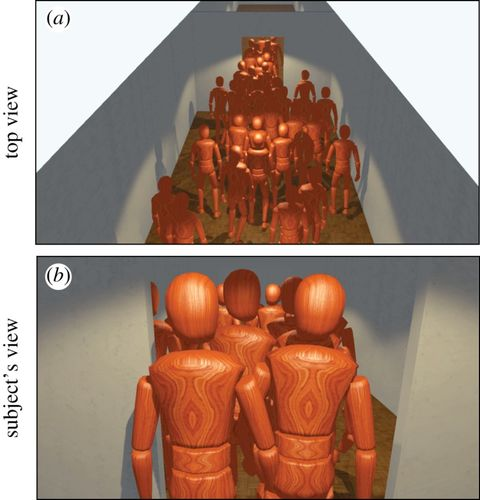
\includegraphics[width=0.30\textwidth]{images/soa/bottleneck_experiment.jpg}
\caption[A bottleneck experiment in a virtual environment]{A bottleneck evacuation experiment in a virtual environment, seen (a) from above and (b) by one participant (Figure~1 of \citet{moussaid2016crowd}, \href{https://creativecommons.org/licenses/by/4.0/}{CC~BY~4.0}, via \href{https://commons.wikimedia.org/}{Wikimedia Commons}).}
\label{fig:soa-bottleneck}
\end{figure}

\section{Discussion}\label{sec:soa-discussion}

The work reviewed covers each element of our problem but not their combination. Boids and steering give cheap and readable motion \citep{reynolds1999steering,reynolds2006big}, crowd models give more realistic motion \citep{vantoll2021algorithms}, the engine offers decisions with navigation and object reservation \citep{epicgames2026statetree,epicgames2026smartobjects}, timed purpose comes from activity-driven crowds \citep{shao2007autonomous,allbeck2010carosa,horni2016matsim}, and queueing theory deals with contention \citep{little1961proof}.

What is missing is the combination of these elements in one game-engine system, in which the user writes out timed activities for a reusable boids population and the capacity-limited shared resources, rather than the user, determine when each activity actually takes place. Each system in \cref{tab:activity-systems} lacks one of these elements, because the research systems have no capacity, queues or engine, the engine tools leave scheduling and queueing to the developer, and \citet{Agent} have goals but no timing or contention. The next chapter turns that gap into a description of the behavior we want and its functional requirements.

\chapter{Scheduled Pedestrians and Shared Resources}\label{chap:problem}

\section{Introduction}\label{sec:problem-intro}

This chapter states what we want to build and what makes it hard. \Cref{sec:problem-statement} describes the behavior we want the people of a simulated place to show, gives a one-page overview of how we produce that behavior (\cref{sub:problem-overview}) and lists the functional requirements R1 to R7 that follow from it (\cref{sec:problem-requirements}). \Cref{sec:problem-challenges} then discusses the issues that make these requirements hard to meet in a game engine, which in turn guide the design in \cref{chap:contribution} and the assessment in \cref{chap:conclusions}.

\section{Behavior}\label{sec:problem-statement}

We begin with a population of people in the game engine whose movement follows the boids rules, so that they are capable of following a path and of reacting to their neighbors but have no reason to go anywhere. A scenario has four components: the \emph{environment} $E$, the \emph{population} $A$, the \emph{schedule} $S$ and the \emph{configuration} $C$. The environment holds the walking surfaces, walls, gates, exits and resources, such as desks, counters and tables, each with its own number of places, the schedule is a set of rules, and the configuration sets the clock speed and the optional behaviors. A rule is of the form $r = (a_r, t_r, \alpha_r, g_r)$, where $a_r$ is the person or group of people that the rule applies to, $t_r$ is the authored time of day, $\alpha_r$ is the action and $g_r$ is the target. The rule becomes \emph{eligible} at $e_r = t_r + o_{a}$, where $o_{a} \geq 0$ is an optional per-person offset. The simulation decides when the rule is \emph{dispatched}, at $d_r \geq e_r$, and when the activity \emph{starts}, at $s_r = d_r + q_r + w_r + p_r$, where $q_r$ is the time spent waiting for a free place, $w_r$ the time spent walking and $p_r$ the short positioning at the place before the service starts. The \emph{lateness} of the rule is then $\ell_r = d_r - e_r$, as \cref{fig:problem-timeline} shows.

\begin{figure}[H]
\centering
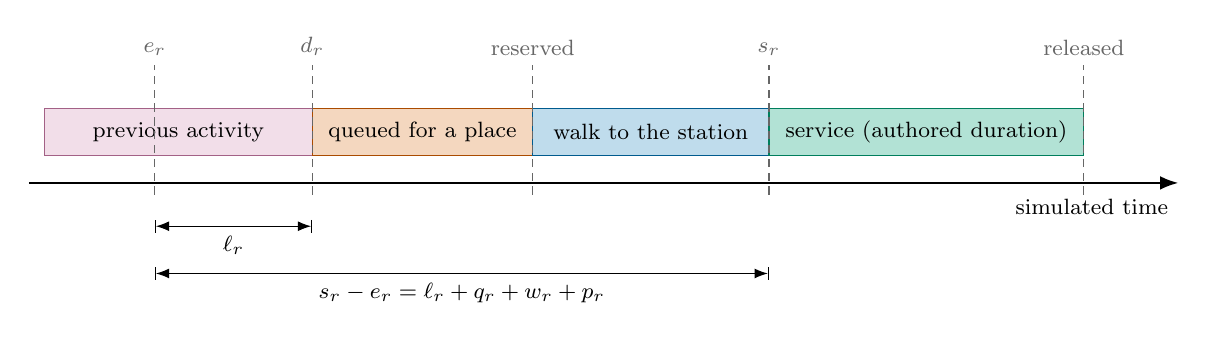
\begin{tikzpicture}[font=\footnotesize,>=Latex,
  tmark/.style={densely dashed,black!60}]
\draw[->,thick] (0,0) -- (14.6,0) node[below left=2pt and 0pt]{simulated time};
\fill[cPurple!25,draw=cPurple!80!black] (0.2,0.35) rectangle (3.6,0.95);
\node at (1.9,0.65) {previous activity};
\fill[cVerm!25,draw=cVerm!80!black] (3.6,0.35) rectangle (6.4,0.95);
\node at (5.0,0.65) {queued for a place};
\fill[cBlue!25,draw=cBlue!80!black] (6.4,0.35) rectangle (9.4,0.95);
\node at (7.9,0.65) {walk to the station};
\fill[cGreen!30,draw=cGreen!80!black] (9.4,0.35) rectangle (13.4,0.95);
\node at (11.4,0.65) {service (authored duration)};
\draw[tmark] (1.6,-0.15) -- (1.6,1.5) node[above]{$e_r$};
\draw[tmark] (3.6,-0.15) -- (3.6,1.5) node[above]{$d_r$};
\draw[tmark] (6.4,-0.15) -- (6.4,1.5) node[above]{reserved};
\draw[tmark] (9.4,-0.15) -- (9.4,1.5) node[above]{$s_r$};
\draw[tmark] (13.4,-0.15) -- (13.4,1.5) node[above]{released};
\draw[|<->|] (1.6,-0.55) -- node[below]{$\ell_r$} (3.6,-0.55);
\draw[|<->|] (1.6,-1.15) -- node[below]{$s_r - e_r = \ell_r + q_r + w_r + p_r$} (9.4,-1.15);
\end{tikzpicture}
\caption[Timeline of one rule that uses a shared resource]{Timeline of one rule that uses a shared resource, where the short positioning $p_r$ is too small to draw (schematic, not measured data).}
\label{fig:problem-timeline}
\end{figure}

\emph{Given $E$, $A$, $S$ and $C$, the system has to turn the rules into movement and activity such that $\ell_r$, $q_r$ and $w_r$ emerge from the people's schedules, their walking, the capacity of the resources and the layout, rather than being explicitly set by the user. It has to do this with one implementation of a person for all scenarios and have sufficient information for the user to see why an activity started when it did.} A rule is therefore a request that the simulation may defer, and changing the scenario must mean changing $E$, $S$ or $C$, with the person remaining the same.

\subsection{Overview of the approach}\label{sub:problem-overview}

Our approach treats every person in the simulation as someone with a timetable rather than as a particle in a flock. For each person or group of people, a user writes a list of activities, each with the time of day from which it may start and the place where it happens, such as a desk in an office from 08:40 for fifteen minutes or a table in a food court at lunchtime. Nothing in this list says how the person gets there or what happens when the place is taken, because those answers come from the rest of the simulation, whose parts and the signals between them are shown in \cref{fig:architecture}.

When an activity becomes due and the person is free, the person picks a route to the place and walks it, spreading out from the people around them without being pulled off the route by the crowd. Every shared place, such as a desk, a counter, a table or an exit, has a limited number of places, a first-come queue and a service time. A person asks for a place as soon as the activity starts and either receives one at once or joins the queue. Once the place is theirs, the person walks to it, stays for the service time and then frees it, which lets the next person in the queue take the place and lets the person move on to the next step of the activity or to the next item of the timetable. A person who is still busy with something else, such as walking, queueing or being served, keeps the next item waiting until they are free, while an item that has become far too late is dropped.

\begin{figure}[H]
\centering
\begin{adjustbox}{max width=0.8\textwidth}
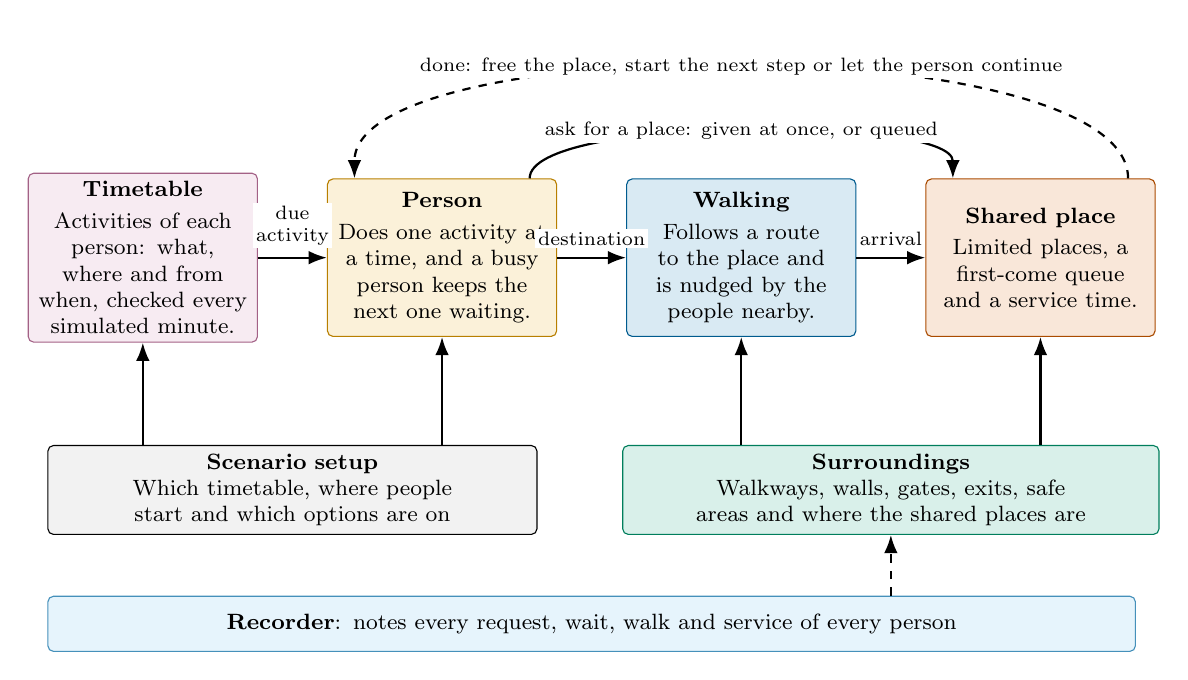
\begin{tikzpicture}[font=\footnotesize,>=Latex,
  every node/.append style={execute at begin node={\hyphenpenalty=10000\relax}},
  box/.style={draw,rounded corners=2pt,align=center,text width=2.7cm,minimum height=2.0cm,inner sep=3pt},
  wide/.style={draw,rounded corners=2pt,align=center,inner sep=3pt,minimum height=.9cm},
  lab/.style={font=\scriptsize,fill=white,inner sep=1pt,align=center},
  arr/.style={->,thick},
  fb/.style={->,thick,dashed}]
\node[box,fill=cPurple!15,draw=cPurple!80!black] (sched) at (0,0) {{\bfseries Timetable}\\[2pt]Activities of each person: what, where and from when, checked every simulated minute.};
\node[box,fill=cOrange!15,draw=cOrange!80!black] (person) at (3.8,0) {{\bfseries Person}\\[2pt]Does one activity at a time, and a busy person keeps the next one waiting.};
\node[box,fill=cBlue!15,draw=cBlue!80!black] (move) at (7.6,0) {{\bfseries Walking}\\[2pt]Follows a route to the place and is nudged by the people nearby.};
\node[box,fill=cVerm!15,draw=cVerm!80!black] (station) at (11.4,0) {{\bfseries Shared place}\\[2pt]Limited places, a first-come queue and a service time.};
\draw[arr] (sched) -- node[lab,above=3pt]{due\\activity} (person);
\draw[arr] (person) -- node[lab,above=3pt]{destination} (move);
\draw[arr] (move) -- node[lab,above=3pt]{arrival} (station);
\draw[arr] ($(person.north east)+(-.35,0)$) .. controls +(0,.8) and +(0,.8) .. node[lab,pos=.5]{ask for a place: given at once, or queued} ($(station.north west)+(.35,0)$);
\draw[fb] ($(station.north east)+(-.35,0)$) .. controls +(0,1.9) and +(0,1.9) .. node[lab,pos=.5]{done: free the place, start the next step or let the person continue} ($(person.north west)+(.35,0)$);
\node[wide,text width=6.6cm,fill=cGreen!15,draw=cGreen!80!black] (env) at (9.5,-2.95) {{\bfseries Surroundings}\\Walkways, walls, gates, exits, safe areas and where the shared places are};
\node[wide,text width=6.0cm,fill=black!5] (cfg) at (1.9,-2.95) {{\bfseries Scenario setup}\\Which timetable, where people start and which options are on};
\draw[arr] (env.north -| move) -- (move.south);
\draw[arr] (env.north -| station) -- (station.south);
\draw[arr] (cfg.north -| sched) -- (sched.south);
\draw[arr] (cfg.north -| person) -- (person.south);
\node[wide,text width=13.6cm,minimum height=.7cm,fill=cSky!15,draw=cSky!80!black] (obs) at (5.7,-4.65) {{\bfseries Recorder}: notes every request, wait, walk and service of every person};
\draw[fb] (obs.north -| env.south) ++(0,0) -- (env.south);
\end{tikzpicture}
\end{adjustbox}
\caption[Overview of the approach]{Overview of the approach, where the dashed arrow at the top is the signal that lets a person continue once an activity is done.}
\label{fig:architecture}
\end{figure}

The surroundings shape all of this without appearing in the timetable, as walkways set the preferred routes, walls and closed gates block them, exits and safe areas take over when an alarm sounds, and the number and position of the shared places decide where queues form. A separate setup for each scenario only says which timetable to use and where people start. A recorder notes every request, wait, walk and service, so that the gap between the written time of an activity and the time it really started can be explained afterwards. The written time is therefore a request rather than an order, and the actual start depends on what the person is still doing, how far they have to walk and whether the place is free, which is exactly the gap that the evaluation in \cref{chap:applications} measures.

\subsection{Functional requirements}\label{sec:problem-requirements}

\Cref{tab:requirements} lists the functional requirements that this behavior implies. None of them ask for realistic behavior, collision-free motion or the ability to predict a real facility.

\section{Issues}\label{sec:problem-challenges}

\subsection{Purpose versus motion}\label{sub:challenge-purpose}

Boids react to the neighbors in their field of view \citep{reynolds1987flocks}, while purpose is global, individual, and changes throughout the day. If goal forces are added to the steering sum, the flock can pull people away from their goals through weights that mean nothing to the user, and hard-coded purpose turns every activity into a separate piece of code. With the separation of action selection and steering \citep{reynolds1999steering}, purpose should be in the form of readable rules external to the person (using a small vocabulary, \textbf{R1}). Reaching a target around walls and roads requires a path over a navigation mesh \citep{snook2000simplified,mononen2009recast}, but a person who only follows a path loses all the local interactions of the boids. The path will dictate where the person goes, and the boids will dictate how they get through others, while the environment will define which surfaces are preferred and which routes are available (\textbf{R5}).

\begin{table}[H]
\centering
\small
\renewcommand{\arraystretch}{1.1}
\begin{tabular}{|L{0.05\textwidth}|L{0.22\textwidth}|L{0.66\textwidth}|}
\hline
\rowcolor{headgray}\textbf{ID} & \textbf{Name} & \textbf{Requirement} \\
\hline
R1 & Purpose as authored data & Which people do what, when and where is stated in readable files, such as XML schedules, apart from the simulation code, with a small fixed set of actions, and changing activities needs no recompilation. \\ \hline
R2 & Timing under contention & An authored time is the earliest start. Eligible, deferred, dispatched, used-up and dropped rules are defined, no authored minute is skipped, realized times result from the simulation, and durations keep their meaning in every run mode. \\ \hline
R3 & Shared capacity-limited resources & Resources have places, a waiting discipline and a service time, people reserve or queue, places are released on completion or interruption, and multi-stage activities advance on completion. \\ \hline
R4 & Reuse across scenarios & One implementation of a person, one movement layer and one resource model serve different maps and activity patterns, and scenario-specific code is small, isolated and identifiable. \\ \hline
R5 & Environmental constraints & Surfaces, walls, gates, exits and the number of resources shape movement and timing without being restated in rules, and people follow paths while boids shape local motion. \\ \hline
R6 & Observability and measurement & Runs record authored, eligible and realized times, resource events, frame timings and the state of every person in files analysable outside the engine, with documented measures. \\ \hline
R7 & Interactive performance & Scenarios run at 30 frames per second with their authored populations, a faster non-visual mode exists, and cost is measurable as the population grows. \\ \hline
\end{tabular}
\caption[Functional requirements]{Functional requirements that follow from the behavior we want.}
\label{tab:requirements}
\end{table}

\subsection{Timing under contention}\label{sub:challenge-timing}

At 08:40, a person could still be walking from home or could still be waiting, as someone else has the desk. Executing the rule anyway would break the routine, executing the rules strictly in order could delay the shift for the whole day, and waiting indefinitely would let the morning rules run in the afternoon. The system has to define when a rule is eligible, when it is deferred, when it is used up, and when it is dropped. No authored minute may be skipped, even when one frame covers several simulated minutes, and the durations must have the same meaning in every run mode (\textbf{R2}).

\subsection{Shared resources and queues}\label{sub:challenge-resources}

\begin{wrapfigure}{r}{0.5\textwidth}
\centering
\vspace{-0.6\baselineskip}
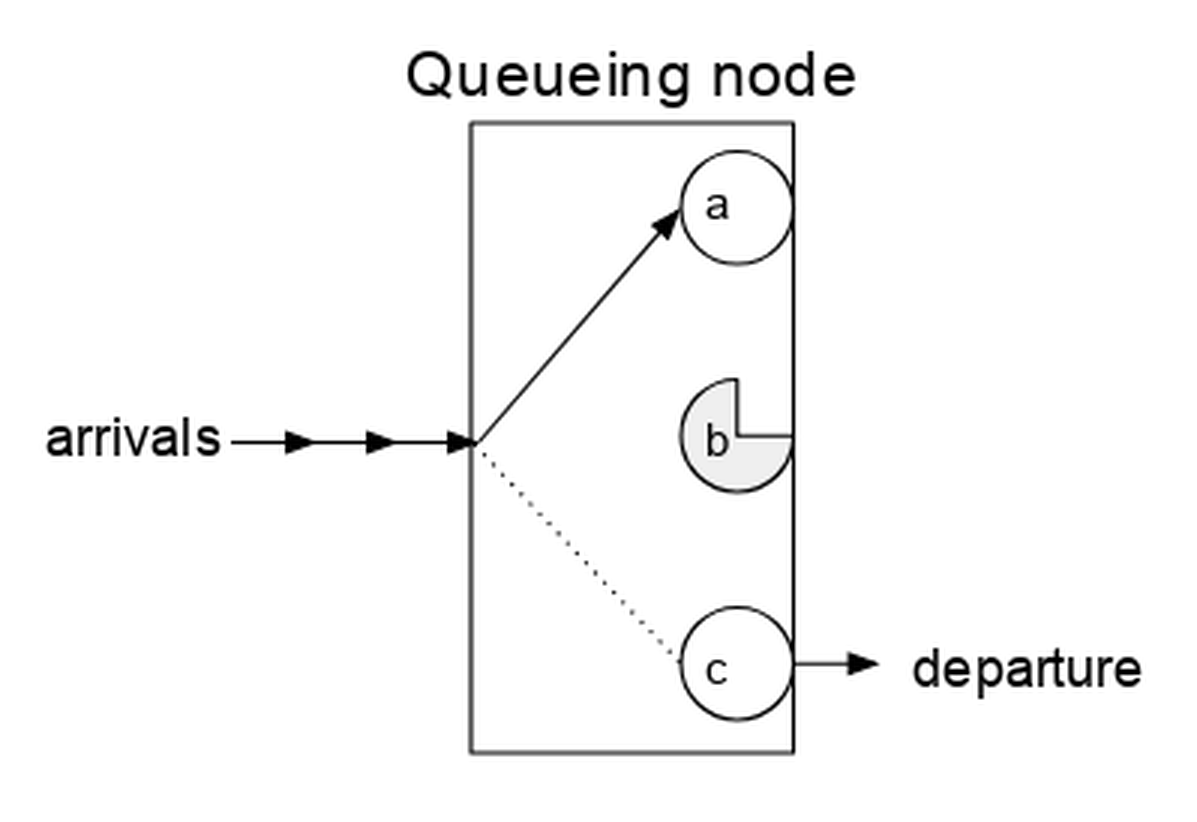
\includegraphics[width=0.48\textwidth]{images/web/queueing_node_x3.png}
\caption[A queueing node]{A queueing node, where arrivals wait for one of several servers and leave after their service (diagram by Dt-rush-8, \href{https://creativecommons.org/licenses/by-sa/4.0/}{CC~BY-SA~4.0}, via \href{https://commons.wikimedia.org/}{Wikimedia Commons}).}
\label{fig:problem-queue}
\vspace{-0.6\baselineskip}
\end{wrapfigure}
Desks, counters, tables and exits are all servers with a capacity, an arrival process, driven here by schedules and walking, and a service time \citep{kendall1953stochastic} (\cref{fig:problem-queue}). The design must decide whether a place is booked on request or on arrival, where the person queues and for which station, and what releases the place. It must also handle a two-stage activity, such as ordering and then eating, so that a person does not hold a table while still queueing at the counter. Smart objects hold the information needed to use them \citep{kallmann1999modeling}, and Unreal Engine's Smart Objects let people claim a slot \citep{epicgames2026smartobjects}. We also need capacity, a queue and a timed service linked to the schedule, with a lifecycle detailed enough to measure the time spent waiting (\textbf{R3}).


\subsection{Reuse across scenarios}\label{sub:challenge-reuse}

The same implementation of a person, movement layer and resource model should serve a daily urban routine, a shopping center, an evacuation and a directed-flow test, with the variations expressed in schedules, maps and configuration. Full reuse is difficult, because an evacuation needs exit choice and a routine needs a home, so scenario-specific code should be small and identifiable (\textbf{R4}), and the environment should absorb variations such as an extra table or a gate opened by a button (\textbf{R5}).

\subsection{Measurement and performance}\label{sub:challenge-measurement}\label{sub:challenge-performance}

A person who stands still could be queued, deferred, blocked or stuck, so watching a run does not reveal their state. The system must therefore record rule times, station events, trips and frame times, document what each measure means and reproduce the analysis from the files (\textbf{R6}). It also shares each 33~ms frame with rendering and animation, and naive boids compare every pair of people (\cref{sub:complexity}), so the scenarios must run interactively at a cost that can be measured (\textbf{R7}).


\part{Core of the Dissertation}

\chapter{A Rule-Authoring Framework for Pedestrian Activity}\label{chap:contribution}
\begingroup\sloppy

\section{Introduction}\label{sec:contrib-intro}

The framework separates four concerns that a crowd demonstration usually mixes in one controller, following the overview of \cref{sub:problem-overview}. These are \emph{what} the person should do and \emph{when} (the schedules), \emph{how} they get there (path-guided hybrid boids), \emph{whether} the activity can take place at that moment (capacity-limited stations) and \emph{what the place actually allows} (the environment). \Cref{tab:requirements-map} shows how the mechanisms of the framework map onto the functional requirements of \cref{chap:problem}.

\begin{table}[H]
\centering
\small\renewcommand{\arraystretch}{1.15}
\begin{tabularx}{\textwidth}{|L{4.3cm}|>{\raggedright\arraybackslash}X|}
\hline
\rowcolor{headgray}\textbf{Requirement} & \textbf{Where it is addressed} \\
\hline
R1 Purpose as authored data & XML schedules with timed, per-person and cohort rules (\cref{sec:schedules}), six actions (\cref{sec:actions}). \\ \hline
R2 Timing under contention & Eligibility, deferral, consumption at dispatch, stale skip (\cref{sec:schedules}), minute-by-minute clock (\cref{sec:clock-modes}). \\ \hline
R3 Shared capacity-limited resources & Stations, areas, super stations and pipelines with reservation, FIFO queue and timed service (\cref{sec:stations}). \\ \hline
R4 Reuse across scenarios & One class for every person, one parser and one station model, scenario managers that prepare each map (\cref{sec:arch-modules,sec:scenario-managers}). \\ \hline
R5 Environment constraints & Sidewalk filter, gates and buttons, exits, safe zones (\cref{sec:environment}), \texttt{Interact} (\cref{sec:actions}). \\ \hline
R6 Observability and measurement & Summary exports and a validation panel, and for the evaluation a run recorder on the test branch (\cref{sec:instrumentation}). \\ \hline
R7 Interactive performance & Visual and Accurate modes (\cref{sec:clock-modes}) and bounded boids blending, measured by a stress test on the test branch. \\ \hline
\end{tabularx}
\caption[Requirements and where they are addressed]{Requirements and where the framework addresses them.}
\label{tab:requirements-map}
\end{table}

\Cref{sec:first-impl} describes the first approach, built before the dissertation, and the two changes that came out of it. \Cref{sec:second-impl} then describes the current pedestrian movement simulator, from its schedules, actions, movement, stations and environment to its clock and run modes, configuration and instrumentation, and \cref{sec:contrib-summary} sums up the chapter.

\section{First Approach}\label{sec:first-impl}

The work started from a prototype built during the pre-dissertation phase, in which a flock of boids moved through a city map and external rules tried to give it purpose. Its rules were organized around categories of places rather than around people. An XML file gave each object of the level a role, such as home, workplace, food place or walkable surface, with fixed active periods such as a morning shift, and during an active period every boid went to a random place of the matching category. Purpose therefore belonged to the period and the type of place rather than to a particular person, and nothing represented a resource that people could share or wait for. Since the boids flocked as one group and steered straight to their destination, a boid that left its group was either held back by its neighbors or dragged them along.

The current system changes both aspects, as rules now name the person, or the group of people, they belong to, give the time of day from which an activity may start and address places through tags and stations with capacities, queues and service times (\cref{sec:schedules,sec:stations}). Movement became individual, as each person follows their own navigation path and the boids rules only bend their heading by a bounded angle, so that the flock spreads people around one another without deciding where they go (\cref{sec:boid-rules}).

\section{Pedestrian Movement Simulator Architecture}\label{sec:second-impl}

The current system replaced the prototype step by step, starting with a schedule manager that gives named people timed tasks. Navigation paths, areas and stations, the scenarios, the hybrid blend, super groups and super stations followed, and finally the simulated clock, the run modes and the action objects, while the division of responsibilities of \cref{fig:architecture} stayed the same throughout.

\subsection{Architecture and Module Layout}\label{sec:arch-modules}

All code lives in one runtime module, \texttt{Thesis}, which uses the engine's \texttt{XmlParser}, \texttt{AIModule} and \texttt{NavigationSystem} modules. \Cref{fig:class-layout} groups the classes by layer, with Unreal's prefixes for actors (\texttt{A}), objects and subsystems (\texttt{U}), structures (\texttt{F}) and interfaces (\texttt{I}).

\texttt{USimulationFeatureRegistry} loads \texttt{SimulationConfig.xml} on every Play, holds the feature flags and settings and answers every other class that asks whether a feature is on. \texttt{AScheduleManager}, one per level, owns the clock, loads the schedule, keeps a registry of people by identifier and evaluates the due rules once per simulated minute. \texttt{ABoidsAB} is the only class that represents a person. As an \texttt{ACharacter}, it leaves walking, gravity and collision with the world to the engine's character movement component. It has a 300\,cm perception sphere for its boids neighbors and an \texttt{AgentId}, usually \texttt{Agent\_N}, that links it to the schedule, and it carries optional components for needs, the priority selector, failure handling, leadership, the police-and-robbers role and greetings, so that one Blueprint of a person serves every scenario. Stations, areas and environment actors are placed in the level and found by tag, spawners create the people and an identifier manager names them in spawn order. Scenario managers prepare a run rather than drive it: at its start, they pick the schedule file, assign homes or entrances and place the people there, set station capacities and start the analytics sessions. Later, the emergency manager raises the alarm and runs the countdown, while each person chooses their own exit and walks there.

\begin{figure}[H]
\centering
\begin{adjustbox}{max width=\textwidth}
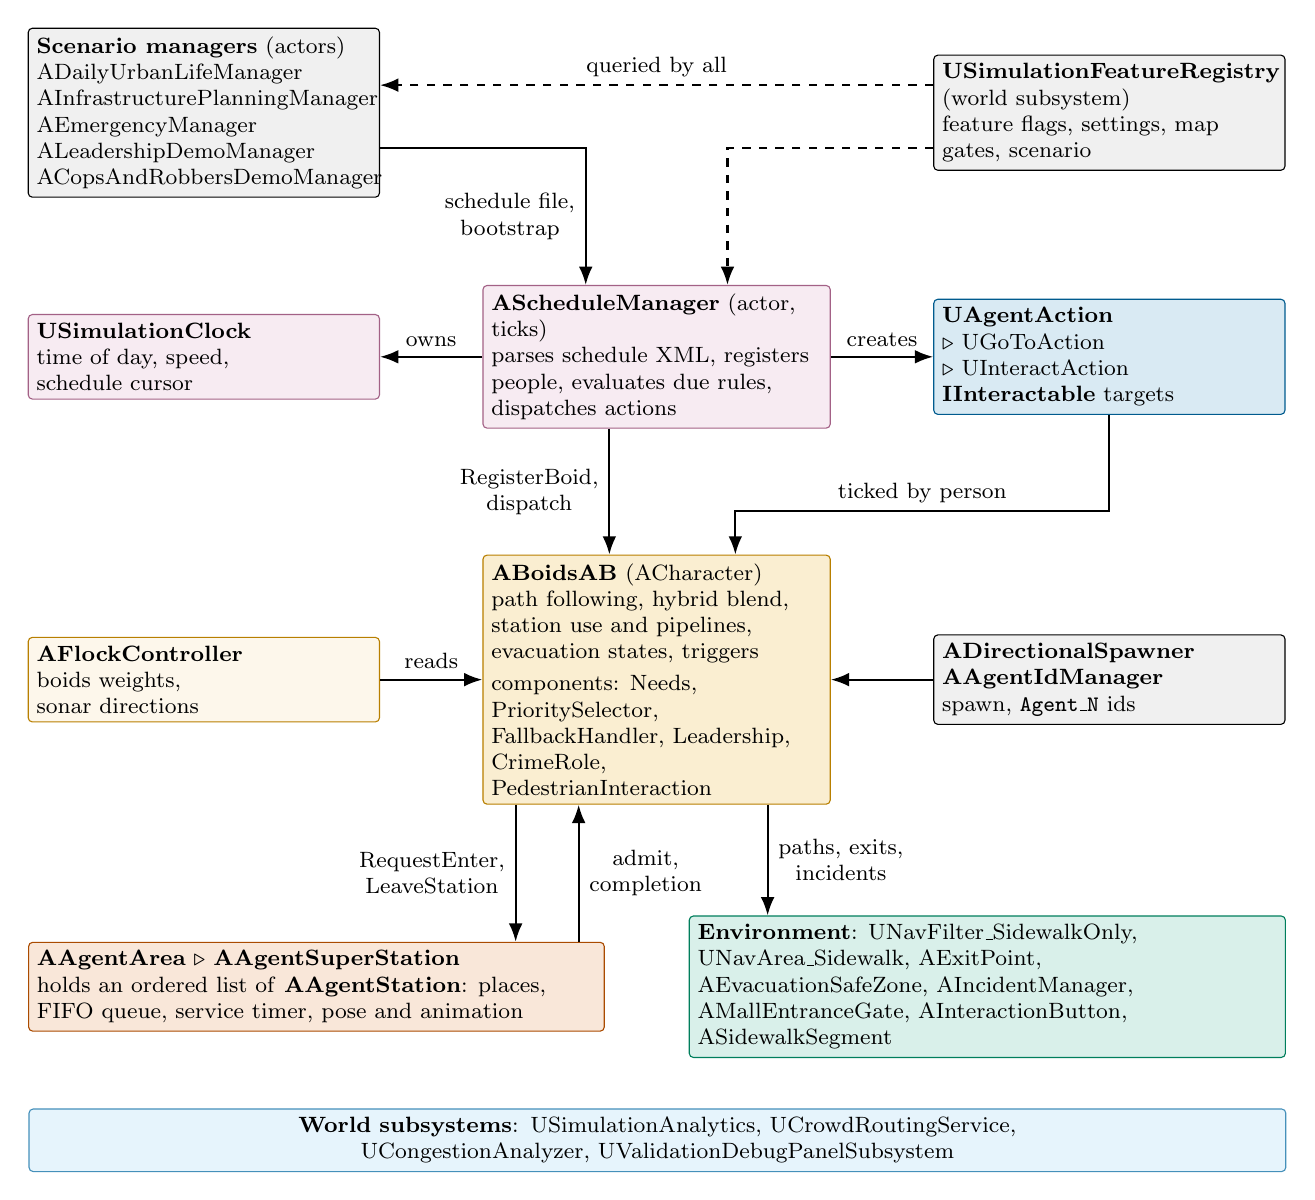
\begin{tikzpicture}[font=\footnotesize,>=Latex,
  every node/.append style={execute at begin node={\hyphenpenalty=10000\relax}},
  cls/.style={draw,rounded corners=1.5pt,align=flush left,inner sep=3pt,fill=black!3},
  lab/.style={fill=white,inner sep=1.5pt,align=center},
  arr/.style={->,thick},
  qry/.style={->,thick,dashed}]
% Three columns (centres 2.24, 7.99 and 13.74 cm); arrows run in the gaps between the boxes.
\node[cls,text width=4.25cm,fill=black!6] (mgr) at (2.24,0) {\textbf{Scenario managers} (actors)\\ADailyUrbanLifeManager\\AInfrastructurePlanningManager\\AEmergencyManager\\ALeadershipDemoManager\\ACopsAndRobbersDemoManager};
\node[cls,text width=4.25cm,fill=black!6] (reg) at (13.74,0) {\textbf{USimulationFeatureRegistry}\\(world subsystem)\\feature flags, settings, map gates, scenario};
\node[cls,text width=4.25cm,fill=cPurple!15,draw=cPurple!80!black] (clk) at (2.24,-3.1) {\textbf{USimulationClock}\\time of day, speed,\\schedule cursor};
\node[cls,text width=4.2cm,fill=cPurple!15,draw=cPurple!80!black] (sm) at (7.99,-3.1) {\textbf{AScheduleManager} (actor, ticks)\\parses schedule XML, registers people, evaluates due rules, dispatches actions};
\node[cls,text width=4.25cm,fill=cBlue!15,draw=cBlue!80!black] (act) at (13.74,-3.1) {\textbf{UAgentAction}\\$\triangleright$ UGoToAction\\$\triangleright$ UInteractAction\\\textbf{IInteractable} targets};
\node[cls,text width=4.2cm,fill=cOrange!18,draw=cOrange!80!black] (person) at (7.99,-7.2) {\textbf{ABoidsAB} (ACharacter)\\path following, hybrid blend, station use and pipelines, evacuation states, triggers\\[2pt]components: Needs, PrioritySelector, FallbackHandler, Leadership, CrimeRole, PedestrianInteraction};
\node[cls,text width=4.25cm,fill=cOrange!8,draw=cOrange!80!black] (flock) at (2.24,-7.2) {\textbf{AFlockController}\\boids weights,\\sonar directions};
\node[cls,text width=4.25cm,fill=black!6] (spawn) at (13.74,-7.2) {\textbf{ADirectionalSpawner}\\\textbf{AAgentIdManager}\\spawn, \texttt{Agent\_N} ids};
\node[cls,text width=7.1cm,fill=cVerm!15,draw=cVerm!80!black] (st) at (3.67,-11.1) {\textbf{AAgentArea} $\triangleright$ \textbf{AAgentSuperStation}\\holds an ordered list of \textbf{AAgentStation}: places, FIFO queue, service timer, pose and animation};
\node[cls,text width=7.36cm,fill=cGreen!15,draw=cGreen!80!black] (env) at (12.19,-11.1) {\textbf{Environment}: UNavFilter\_SidewalkOnly, UNavArea\_Sidewalk, AExitPoint, AEvacuationSafeZone, AIncidentManager, AMallEntranceGate, AInteractionButton, ASidewalkSegment};
\node[cls,text width=15.75cm,align=center,fill=cSky!15,draw=cSky!80!black] (svc) at (8.0,-13.05) {\textbf{World subsystems}: USimulationAnalytics, UCrowdRoutingService, UCongestionAnalyzer, UValidationDebugPanelSubsystem};
\draw[qry] (reg.west |- 0,0.35) -- node[lab,above=1pt]{queried by all} (mgr.east |- 0,0.35);
\draw[qry] (reg.west |- 0,-0.45) -| ($(sm.north)+(0.9,0)$);
\draw[arr] (mgr.east |- 0,-0.45) -| node[lab,pos=0.75,left=2pt]{schedule file,\\bootstrap} ($(sm.north)+(-0.9,0)$);
\draw[arr] (sm.west) -- node[lab,above=2pt]{owns} (clk.east);
\draw[arr] (sm.east) -- node[lab,above=2pt]{creates} (act.west);
\draw[arr] ($(sm.south)+(-0.6,0)$) -- node[lab,left=2pt]{RegisterBoid,\\dispatch} ($(person.north)+(-0.6,0)$);
\draw[arr] (act.south) |- node[lab,pos=0.75,above=1pt]{ticked by person} ($(person.north)+(1.0,0.55)$) -- ($(person.north)+(1.0,0)$);
\draw[arr] (flock.east) -- node[lab,above=2pt]{reads} (flock.east -| person.west);
\draw[arr] (spawn.west) -- (spawn.west -| person.east);
\draw[arr] (person.south -| 6.2,0) -- node[lab,left=2pt]{RequestEnter,\\LeaveStation} (st.north -| 6.2,0);
\draw[arr] (st.north -| 7.0,0) -- node[lab,right=2pt]{admit,\\completion} (person.south -| 7.0,0);
\draw[arr] (person.south -| 9.4,0) -- node[lab,right=2pt]{paths, exits,\\incidents} (env.north -| 9.4,0);
\end{tikzpicture}
\end{adjustbox}
\caption[Classes grouped by layer]{Classes of the second implementation grouped by layer, where solid arrows are calls or ownership and dashed arrows are queries of the configuration registry.}
\label{fig:class-layout}
\end{figure}

In each frame, the schedule manager advances the clock and processes every simulated minute between its cursor and the clock. Each person then updates their current action, their station pose and their needs, lets the priority selector choose the controlling layer and moves along their path. The rest is event-driven, as engine timers in real seconds end station services and timed idles, process exit queues and run the evacuation countdown. People retry registration every 0.2\,s until the manager accepts them, so actor order does not matter.

\subsection{Schedules and the Rule Language}\label{sec:schedules}

A schedule is an XML file in \texttt{Project/Schedules/} that tells named people what to do and from when. The schedule manager of each level names its file, and the Daily Urban Life and infrastructure managers can replace it with a file named in the configuration. A schedule has a root \texttt{<schedule>} with \texttt{<agent id="Agent\_N">} and \texttt{<superGroup>} blocks, a person has \texttt{<rule time="HH:MM">} elements, and each rule may have an \texttt{<if condition="..."/>}, a \texttt{<then action="A" .../>} and an \texttt{<else>} alternative. A \texttt{UseStation} action may have \texttt{<stage>} children, and a super group has a \texttt{<members>} list and its own rules, and \cref{tab:grammar} lists every element with its attributes. Element names are case-insensitive, but attribute names must be spelled exactly, and a missing or malformed file is logged and leaves the people without rules.

\begin{table}[H]
\centering
\small\renewcommand{\arraystretch}{1.15}
\begin{tabularx}{\textwidth}{|L{2.3cm}|L{4.4cm}|>{\raggedright\arraybackslash}X|}
\hline
\rowcolor{headgray}\textbf{Element} & \textbf{Attributes (default)} & \textbf{Meaning} \\
\hline
\texttt{schedule} & none & Root of the file, holding \texttt{agent} and \texttt{superGroup} blocks. \\ \hline
\texttt{agent} & \texttt{id} (required) & The rules of one person, whose \texttt{id} must equal the runtime identifier \texttt{Agent\_N}. \\ \hline
\texttt{superGroup} & \texttt{id} & A cohort whose \texttt{members} list names people with \texttt{<agent ref="Agent\_N"/>}, each of whom receives a copy of the group's rules. \\ \hline
\texttt{rule} & \texttt{time} (00:00), \texttt{prob} (1.0) & The time of day from which the rule may run, where malformed text gives 00:00 and out-of-range values are clamped, and a probability rolled at every attempt, where a failed roll uses up the rule. \\ \hline
\texttt{if} & \texttt{condition} (none) & \texttt{emergency == true|false} or \texttt{location == Home|Work|Food}, which selects \texttt{then} or \texttt{else}. \\ \hline
\texttt{then}, \texttt{else} & \texttt{action}, \texttt{area} or \texttt{superStation} or \texttt{target}, \texttt{stationType}, \texttt{duration} ($-1$), \texttt{id} & One of the six actions of \cref{tab:actions}, its target tag (the first of the three that is given), a station identifier or tag inside the area, a duration in simulated minutes ($\le 0$ gives an indefinite idle or the station's default of 5) and, for \texttt{Trigger}, the trigger name. \\ \hline
\texttt{stage} & \texttt{area} or \texttt{superStation}, \texttt{stationType}, \texttt{duration} & One step of a \texttt{UseStation} pipeline, with the same meaning as above. \\ \hline
\end{tabularx}
\caption[Elements of the schedule language]{Elements of the schedule language with their attributes and defaults.}
\label{tab:grammar}
\end{table}

\Cref{lst:dul-agent0} is the full schedule of one office worker in the Daily Urban Life scenario. The worker uses a bed in the \texttt{Sleep} area, walks to the office area \texttt{Work0}, sits at desk \texttt{A0} for 15 simulated minutes, takes a break, works a second block, walks home and goes back to bed. The gaps between the rules allow for walking, and the evaluation measures whether they are long enough, since a rule that comes due while the person is still walking is deferred. The file holds 50 people with 304 rules, and people 25 to 49 repeat the pattern of people 0 to 24 fifteen minutes later on the same desks, so a late first user makes the second user queue. The file creates this contention without any scripting, because it only states who wants which desk and from when.

\begin{lstlisting}[language=XML,basicstyle=\ttfamily\scriptsize,caption={Schedule of \texttt{Agent\_0} in \texttt{DailyUrbanLifeSchedule.xml}, complete.},label={lst:dul-agent0}]
<agent id="Agent_0">
 <rule time="08:05"><then action="UseStation" area="Sleep" stationType="Bed1" duration="20"/></rule>
 <rule time="08:22"><then action="MoveTo" area="Work0"/></rule>
 <rule time="08:40"><then action="UseStation" area="Work0" stationType="A0" duration="15"/></rule>
 <rule time="09:00"><then action="Trigger" id="Break"/></rule>
 <rule time="09:13"><then action="UseStation" area="Work0" stationType="A0" duration="15"/></rule>
 <rule time="09:43"><then action="MoveTo" area="Home1"/></rule>
 <rule time="09:55"><then action="UseStation" area="Sleep" stationType="Bed1" duration="20"/></rule>
</agent>
\end{lstlisting}

\Cref{lst:malla-pipeline} is one shopper in Mall A, whose lunch rule in the super station \texttt{FoodCourt} has two stages, 10 minutes at a counter and then 14 minutes at a table. The table is sought only when the counter service has finished, so a queue at the counter delays the search for a table. The two \texttt{<stage>} elements are children of the rule's single \texttt{<then>}, which the closing \texttt{</then>} ends, and the rule needs no \texttt{<else>} because a rule without an \texttt{<if>} always runs its \texttt{<then>}. A \texttt{<superGroup>} is written in the same way, with a \texttt{<members>} list before the rules, and each corridor map has one or two of them, one per cohort.

\begin{lstlisting}[language=XML,basicstyle=\ttfamily\scriptsize,caption={Schedule of \texttt{Agent\_0} in \texttt{InfrastructurePlanning\-Schedule\_\allowbreak MallA.xml}, complete.},label={lst:malla-pipeline}]
<agent id="Agent_0">
 <rule time="08:02"><then action="Idle" duration="8"/></rule>
 <rule time="08:12"><then action="MoveTo" area="ShopA"/></rule>
 <rule time="08:22"><then action="UseStation" area="ShopA" stationType="ShopA_Desk" duration="10"/></rule>
 <rule time="08:36"><then action="MoveTo" area="FoodCourt"/></rule>
 <rule time="08:46">
  <then action="UseStation">
   <stage superStation="FoodCourt" stationType="FoodCounter" duration="10"/>
   <stage superStation="FoodCourt" stationType="FoodTable" duration="14"/>
  </then>
 </rule>
 <rule time="09:16"><then action="MoveTo" area="Exit1"/></rule>
</agent>
\end{lstlisting}

A rule is \emph{due} at the processed minute $M$ of day $D$ if it has not been consumed on day $D$ and its effective minute is not later than $M$:
\begin{equation}
\boxed{\mathrm{due}(r, M, D) \iff \mathrm{LastExecutedDay}(r) \neq D \;\wedge\; (t_r + o_a) \bmod 1440 \le M}
\label{eq:due}
\end{equation}
where $t_r$ is the authored time in minutes since midnight and $o_a$ is the person's schedule offset. For each person, the manager visits the due rules in time order and makes one attempt per rule, which either \emph{dispatches} it (its action starts), \emph{defers} it (it is tried again at the next minute) or \emph{consumes} it without dispatch. Before any other check, a rule of a person who is present and not busy is consumed as stale when more than 45 minutes have passed since its effective minute, while the rules of a person who has not spawned yet are kept until that person appears. A busy person is never stale-skipped, so an hour in a queue does not cost them every rule that came due meanwhile, and the window, set by hand, stops a long morning delay from releasing morning activities into the afternoon. The probability is then rolled at every attempt, so a rule deferred $k$ times is dispatched with probability $p^{k+1}$ rather than $p$, although no shipped schedule sets \texttt{prob}, and a false condition runs the \texttt{<else>} action if there is one and otherwise consumes the rule.

\Cref{tab:deferral} lists the checks that defer a rule, in the order they are applied. The exemptions matter as much as the checks, because \texttt{StartEvacuation} must not wait for anyone, a \texttt{Break} must interrupt a desk, and in Daily Urban Life a commute home must interrupt whatever the person is doing.

\begin{table}[H]
\centering
\small\renewcommand{\arraystretch}{1.15}
\begin{tabularx}{\textwidth}{|l|L{6.0cm}|>{\raggedright\arraybackslash}X|}
\hline
\rowcolor{headgray} & \textbf{Reason} & \textbf{Exemptions} \\
\hline
a & Person not registered with the schedule manager & none \\ \hline
b & Person in an evacuation state (the condition is evaluated after this check) & none \\ \hline
c & An incident or a global evacuation is active in the world & \texttt{StartEvacuation} \\ \hline
d & Person at a station, queued for one, or in a pipeline & \texttt{StartEvacuation}, \texttt{Trigger} \texttt{Break}/\texttt{Pause}, in Daily Urban Life a \texttt{MoveTo} to a \texttt{Home} tag \\ \hline
e & Person's previous action still running & \texttt{StartEvacuation} \\ \hline
f & Critical hunger or energy, an active crime response, or following a leader & in Daily Urban Life, \texttt{MoveTo}/\texttt{Interact} to a \texttt{Home} tag \\ \hline
\end{tabularx}
\caption[Reasons for deferring a due rule]{Reasons for deferring a due rule, in the order they are checked.}
\label{tab:deferral}
\end{table}

Deferral turns walking and queueing time into lateness, since a rule that comes due while the person is still walking waits until the person arrives. It also lets rules run out of the order in which the user wrote them, as when a \texttt{Home} commute, which is exempt from the station check, overtakes a desk rule that is waiting for its desk. A rule is consumed when its action is dispatched, not when the activity ends, so the scheduler never needs to know how an activity ends. A user expresses ``do B after A has finished'' either as stages of one \texttt{UseStation} rule or through deferral, which holds the next rule while the person is busy. A \texttt{<superGroup>} gives each member its own copy of its rules, which are evaluated, deferred and consumed one person at a time, so a cohort saves writing but does not model a collective decision. In Daily Urban Life, each person's rules can be shifted by a random offset of up to 8 minutes, so that people sharing a pattern do not all leave in the same minute.

\subsection{Actions}\label{sec:actions}

The action vocabulary is kept small on purpose (\cref{tab:actions}), because a larger vocabulary would make schedules harder to read and pull scenario logic back into the parser. \texttt{UAgentAction} has four states (not started, running, completed and failed), and a person owns at most one action at a time, so a new action cancels its predecessor. The action object does not move the person but calls the person's normal movement functions and watches the person's state, so movement code stays in one place and deferral check (e) only asks whether the action is still running. A \texttt{GoTo} completes when the person reports arrival or has stopped within 180\,cm of the target, and fails when the person is still moving without a path after 0.5 real seconds, or after 180 real seconds unless it is then within 180\,cm. Every target is a single point, so all people bound for \texttt{Exit1} end at the same point, and any stop of movement sets the arrival flags, which is why the run recorder of the evaluation also logs the remaining distance. \texttt{Interact} needs a target that implements \texttt{IInteractable}, and its only implementation is the Mall B entrance button, which opens a linked gate and so changes the navigation mesh for later path queries.

\begin{table}[H]
\centering
\small\renewcommand{\arraystretch}{1.15}
\begin{tabularx}{\textwidth}{|L{3.4cm}|L{1.3cm}|>{\raggedright\arraybackslash}X|}
\hline
\rowcolor{headgray}\textbf{Action} & \textbf{Object} & \textbf{What happens} \\
\hline
\texttt{MoveTo} / \texttt{GoTo} & yes & Walk to the first actor carrying the tag. Completes on arrival within 180\,cm and fails on path failure or after 180 real seconds (90 simulated minutes in Accurate mode). \\ \hline
\texttt{Interact} & yes & Walk to the target's interaction point, then call \texttt{Interact} on it if it still accepts. \\ \hline
\texttt{Idle} & no & Stop and stay idle for \texttt{duration} simulated minutes (indefinitely if $\le 0$). \\ \hline
\texttt{UseStation} & no & Start a station pipeline of one or more stages (\cref{sec:stations}). \\ \hline
\texttt{Trigger} & no & Raise one of the named triggers \texttt{Break}, \texttt{Pause}, \texttt{Flee}, \texttt{Greet}. \\ \hline
\texttt{StartEvacuation} & no & Start the global evacuation through the emergency manager. \\ \hline
\end{tabularx}
\caption[The six schedule actions]{The six schedule actions, where ``Object'' marks the actions that create a \texttt{UAgentAction}.}
\label{tab:actions}
\end{table}

\texttt{Idle} stops the person and starts a timer, and the mall schedules open with idles of 2 to 10 minutes so that shoppers do not all enter at once. \texttt{Break} and \texttt{Pause} release the person from their station, and in Daily Urban Life a \texttt{Break} sends the person to the plaza. \texttt{UseStation} builds the stage list and starts the station pipeline, and the rule is consumed even if no stage can be built. \texttt{StartEvacuation} calls the emergency manager, which starts a fire incident of global radius, alarms every person and starts the countdown. The call is global and idempotent, so the evacuation schedule is a single rule for \texttt{Agent\_0}, after which check (c) holds every other rule of every person.

\endgroup

% contribution_part2.tex
% Second half of the architecture section: movement, stations, environment, configuration, instrumentation.
\providecommand{\compacttable}{\footnotesize\renewcommand{\baselinestretch}{1}\selectfont\renewcommand{\arraystretch}{1.15}}
\newcolumntype{Q}{>{\raggedright\arraybackslash}X}
\newcolumntype{R}[1]{>{\raggedright\arraybackslash}p{#1}}
% Long code identifiers cannot be hyphenated; allow looser spacing in this part only.
\begingroup\sloppy\setlength{\emergencystretch}{3em}

%======================================================================
\subsection{Movement: capsules, probes and the hybrid blend}
\label{sec:collision-system}\label{sec:boid-rules}

Each person's capsule is moved by the engine's \texttt{CharacterMovementComponent}, which applies gravity and slides it along blocking geometry, and the boids rules see the people who overlap a 300\,cm sphere around the person. There is no grid and no cap on the number of neighbors, so the cost per person grows with local density \citep{reynolds2006big}. None of this is collision avoidance in the pedestrian sense, where each person would choose a velocity that keeps them clear of their neighbors over a time horizon \citep{vandenberg2008reciprocal,vandenberg2011reciprocal,karamouzas2014universal}, so overlaps are possible and capsules deal with contact afterwards. A forward sonar ray of 300\,cm turns the person toward the first free one of 100 precomputed directions when the ray hits an obstacle \citep{reynolds1999steering}. In Visual and Accurate modes (\cref{sec:clock-modes}), two side rays of 95\,cm and a forward ray of 110\,cm also remove any component of movement toward a wall and slide the person along walls they would hit. A person pushed more than 50\,cm off the navigation mesh is projected back onto it at most once per second. The fallback handler retries failed path queries, recomputes the path of a person who covers less than 15\,cm in 6\,s, and lets a fleeing person choose another exit when more than three paths to their queue slot have failed.

In the hybrid blend, the path decides the direction of travel and the flock can only turn it sideways by a bounded angle. The progress direction $\hat{\mathbf{p}}$ points to the point 140\,cm ahead of the person's closest point on their path segment, never backwards along it. The flock force is flattened, normalized and scaled by $w_m=0.35$, its component along $\hat{\mathbf{p}}$ is discarded, the lateral remainder $\mathbf{l}$ is capped at $\tan 18^\circ\approx0.325$, and the new heading is the unit vector
\begin{equation}
\mathbf{h}=\frac{\hat{\mathbf{p}}+\mathbf{l}}{\lVert\hat{\mathbf{p}}+\mathbf{l}\rVert}
\label{eq:blend-heading}
\end{equation}
shown in \cref{fig:blend-geometry}. The forward component is always the full $\hat{\mathbf{p}}$, so the flock can never stop or reverse progress, and the wall probes then refine the direction within the same cone. The blend is switched off in Fast mode, in every evacuation state and while a person is admitted to or queued for a station, so that a worker going to a reserved desk reaches it, and in those cases the path alone decides the direction.

The priority selector decides each frame which layer controls the person (\cref{tab:priority-layers}). Higher layers move the person through the layer's own overrides and defer the person's due rules until the layer releases them, and in our tests crime and leadership were off and needs were frozen, so only the emergency, schedule and idle layers were active. The outcome is two regimes: \emph{free flocking}, where the boids rules alone set the velocity, and \emph{directed travel}, where a rule, need, leader or evacuation provides a target, the path sets the direction and the flock only nudges it. We preferred this to the usual weighted sum of seek and flock forces \citep{reynolds1999steering}, in which a dense group can stall a person or carry them past their turn and the right weights depend on density. The downside is that the flock has little influence during travel, which is when crowding occurs.

\begin{figure}[H]
\centering
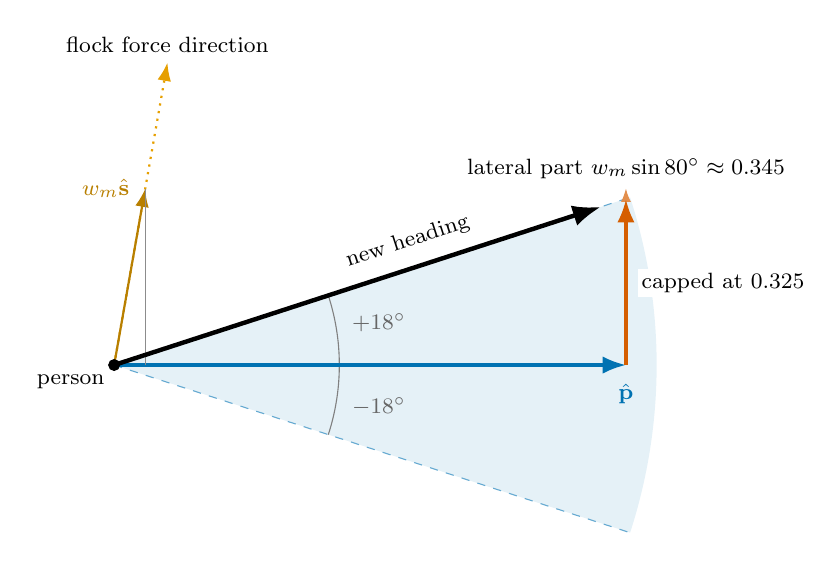
\begin{tikzpicture}[>=Latex,font=\footnotesize,scale=1.3,
  lab/.style={fill=white,inner sep=1.5pt}]
  \fill[cBlue!10] (0,0) -- (18:5.3) arc (18:-18:5.3) -- cycle;
  \draw[cBlue!60,dashed] (0,0) -- (18:5.3);
  \draw[cBlue!60,dashed] (0,0) -- (-18:5.3);
  \draw[black!50] (2.2,0) arc (0:18:2.2);
  \draw[black!50] (2.2,0) arc (0:-18:2.2);
  \node[black!60] at (9:2.62) {$+18^\circ$};
  \node[black!60] at (-9:2.62) {$-18^\circ$};
  \draw[->,very thick,cBlue] (0,0) -- (5,0) node[below=3pt]{$\hat{\mathbf{p}}$};
  \draw[->,dotted,thick,cOrange] (0,0) -- (80:3.0) node[above,text=black]{flock force direction};
  \draw[->,thick,cOrange!80!black] (0,0) -- (80:1.75) node[left=2pt]{$w_m\hat{\mathbf{s}}$};
  \draw[black!45] (0.304,0) -- (0.304,1.723);
  \draw[->,dashed,cVerm!70] (5,0) -- (5,1.723) node[lab,above=2pt,text=black]{lateral part $w_m\sin 80^\circ\approx0.345$};
  \draw[->,very thick,cVerm] (5,0) -- (5,1.62);
  \node[lab,right=4pt] at (5,0.8) {capped at 0.325};
  \draw[->,ultra thick] (0,0) -- (18:5.0) node[pos=0.62,above=2pt,sloped]{new heading};
  \filldraw (0,0) circle (1.5pt) node[below left]{person};
\end{tikzpicture}
\caption[Geometry of the hybrid blend]{Geometry of the hybrid blend, where the heading stays inside the shaded cone around the path. The flock force is drawn at 80\textdegree{} to the path as one example, so its lateral part is $w_m\sin 80^\circ\approx0.345$ and the cap at $\tan 18^\circ\approx0.325$ shortens it.}
\label{fig:blend-geometry}
\end{figure}

\begin{table}[H]
\centering
{\compacttable
\begin{tabularx}{\textwidth}{|l|Q|Q|}
\hline
\rowcolor{headgray}\textbf{Layer} & \textbf{Applies when} & \textbf{Movement and effect on the schedule} \\
\hline
PanicEmergency & fleeing, exiting, awaiting reaction, moving to a safe zone, evacuated or casualty & evacuation movement, all rules deferred \\ \hline
CriticalNeeds & hunger $\ge0.65$ or energy $\le0.35$ & to the nearest food point or home, leaving any station, rules deferred \\ \hline
CrimeResponse & crime feature on and the role wants to pursue, flee or avoid & run to or from the other party, rules deferred \\ \hline
Leadership & leadership feature on and actively following & walk behind the leader, rules deferred if configured \\ \hline
ScheduledTasks & moving or holding a target station & schedule action with the blend \\ \hline
IdleFlock & none of the above & free flocking, or a slow mill near home in Daily Urban Life \\ \hline
\end{tabularx}}
\caption[Priority layers of the person]{Priority layers of the person, highest first.}
\label{tab:priority-layers}
\end{table}

%======================================================================
\subsection{Stations, areas, super stations and pipelines}
\label{sec:stations}

A rule that sends a person to the office has no way of knowing whether a desk will be free, and stations are what keep track of that. They build on smart objects, which hold the logic of their use \citep{kallmann1999modeling,forbus2001notes}, and on Unreal Engine's Smart Objects, whose slots people claim and release \citep{epicgames2026smartobjects}, and they add several places, a first-come, first-served queue and a timed service authored in the schedule. In queueing terms, a station is a multi-server FIFO queue \citep{kendall1953stochastic,shortle2018fundamentals} with two differences from the standard model, as places are booked before the customer arrives and the queue takes up no space. An \texttt{AAgentStation} is one resource, such as a desk, counter, table or bed, with its places, its admitted occupants, including those still walking, and a queue. An \texttt{AAgentArea} groups stations under an actor tag such as \texttt{Work0} in an ordered array, and an \texttt{AAgentSuperStation} is an area of a few interchangeable stations, such as the counters and tables of a food court. A pipeline is the person's list of stages with the index of the current one, and \cref{fig:station-lifecycle} shows one stage.

A stage is resolved to a station only when it starts, so a diner does not hold a table while still queueing at the counter (\cref{lst:malla-pipeline}). \texttt{RequestEnter} admits the person if a place is free and otherwise queues them. Reserving at dispatch prevents two people from walking to the last desk and finding the conflict on arrival, although the desk then sits idle while its user walks and the first person to ask wins even if another is nearer. A queued person becomes idle where they stand and does not walk to the station or line up. An admitted person walks to the station and arrives within 180\,cm horizontally and 220\,cm vertically of it, then snaps or interpolates to the station's interaction point, so that a diner sits at the table rather than beside it, and their service timer and animation start. The service lasts the stage's \texttt{duration} or, if none is given, the station's default of 5 simulated minutes, converted to real seconds for the run mode (\cref{sec:clock-modes}). When it expires, the place is released, the next stage is resolved from where the person stands, and the station admits the head of its queue on its next tick. \texttt{LeaveStation} frees a place or a queue entry when a \texttt{Break}, \texttt{Pause}, home commute, evacuation, need or queue time-out interrupts the person, and while a person is admitted, queued or in a pipeline, their other rules are deferred, which links station waiting to schedule lateness.

A stage resolves to the first open area with the stage's tag and, within it, to the first station in array order whose type matches and that has a free place, or otherwise to the first matching station. A misspelled \texttt{stationType} therefore silently falls back to any station in the area. This policy had two effects in the malls. First, a queued person stays bound to the station chosen at that moment and does not move to an equivalent one that frees earlier. Second, when every station is busy, all new arrivals join the queue of the \emph{first} matching station, so the array order becomes a modeling decision. A queued person gives up after 50 engine seconds and goes home, except in the infrastructure scenario or when \texttt{enableInfrastructureAnalysis} is on, where they wait indefinitely. There is no time-out between admission and arrival, so a place stays reserved until its owner arrives or leaves.

\begin{figure}[H]
\centering
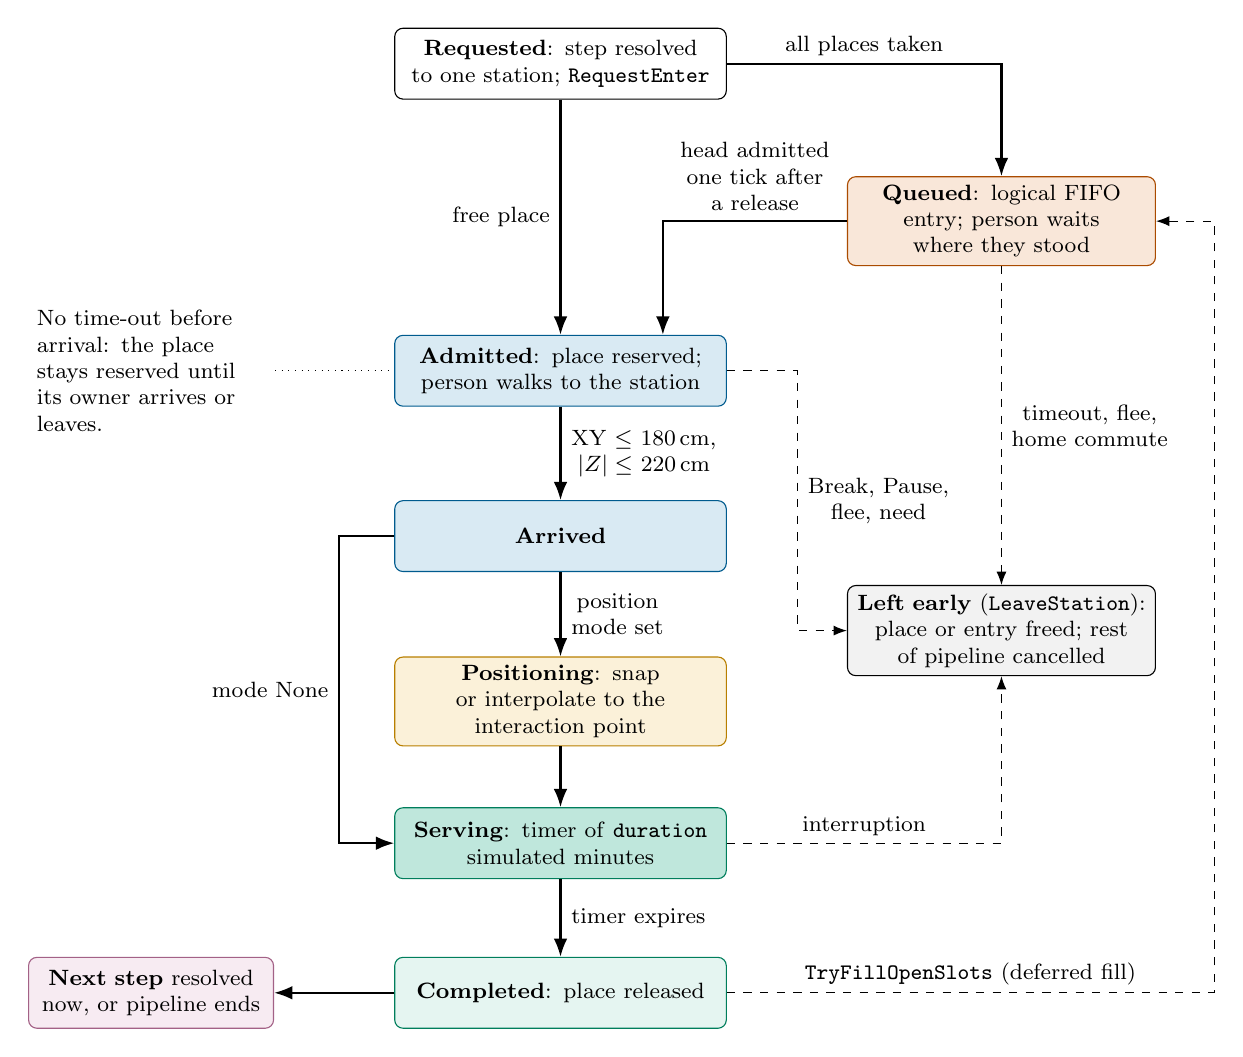
\begin{tikzpicture}[font=\footnotesize,>=Latex,
  every node/.append style={execute at begin node={\hyphenpenalty=10000\relax}},
  st/.style={draw,rounded corners=3pt,align=center,text width=4.0cm,minimum height=0.9cm,inner sep=3pt,fill=white},
  side/.style={draw,rounded corners=3pt,align=center,text width=3.7cm,minimum height=0.9cm,inner sep=3pt,fill=black!5},
  lab/.style={align=center,fill=white,inner sep=1.5pt}]
\node[st] (req) at (0,0) {\textbf{Requested}: step resolved to one station; \texttt{RequestEnter}};
\node[st,fill=cBlue!15,draw=cBlue!80!black] (adm) at (0,-3.9) {\textbf{Admitted}: place reserved; person walks to the station};
\node[st,fill=cBlue!15,draw=cBlue!80!black] (arr) at (0,-6.0) {\textbf{Arrived}};
\node[st,fill=cOrange!15,draw=cOrange!80!black] (pos) at (0,-8.1) {\textbf{Positioning}: snap or interpolate to the interaction point};
\node[st,fill=cGreen!25,draw=cGreen!80!black] (srv) at (0,-9.9) {\textbf{Serving}: timer of \texttt{duration} simulated minutes};
\node[st,fill=cGreen!10,draw=cGreen!80!black] (rel) at (0,-11.8) {\textbf{Completed}: place released};
\node[side,fill=cVerm!15,draw=cVerm!80!black] (que) at (5.6,-2.0) {\textbf{Queued}: logical FIFO entry; person waits where they stood};
\node[side] (left) at (5.6,-7.2) {\textbf{Left early} (\texttt{LeaveStation}): place or entry freed; rest of pipeline cancelled};
\node[side,text width=2.9cm,fill=cPurple!15,draw=cPurple!80!black] (next) at (-5.2,-11.8) {\textbf{Next step} resolved now, or pipeline ends};
\node[align=left,text width=2.9cm] (note) at (-5.2,-3.9) {No time-out before arrival: the place stays reserved until its owner arrives or leaves.};
\draw[->,thick] (req) -- node[lab,left=2pt]{free place} (adm);
\draw[->,thick] (req.east) -| node[lab,pos=0.25,above=1pt]{all places taken} (que.north);
\draw[->,thick] (que.west) -| node[lab,pos=0.25,above=2pt]{head admitted\\one tick after\\a release} ($(adm.north)+(1.3,0)$);
\draw[->,thick] (adm) -- node[lab,right=2pt]{XY $\le$ 180\,cm,\\$|Z|\le$ 220\,cm} (arr);
\draw[->,thick] (arr) -- node[lab,right=2pt]{position\\mode set} (pos);
\draw[->,thick] (arr.west) -- ++(-0.7,0) |- node[lab,pos=0.25,left=2pt]{mode None} (srv.west);
\draw[->,thick] (pos) -- (srv);
\draw[->,thick] (srv) -- node[lab,right=2pt]{timer expires} (rel);
\draw[->,thick] (rel) -- (next);
\draw[->,dashed] (rel.east) -- node[lab,above=1pt]{\texttt{TryFillOpenSlots} (deferred fill)} (8.3,-11.8) |- (que.east);
\draw[->,dashed] (que.south) -- node[lab,right=2pt]{timeout, flee,\\home commute} (left.north);
\draw[->,dashed] (adm.east) -- ++(0.9,0) |- node[lab,pos=0.25,right=2pt]{Break, Pause,\\flee, need} (left.west);
\draw[->,dashed] (srv.east) -| node[lab,pos=0.25,above=1pt]{interruption} (left.south);
\draw[dotted] (note.east) -- (adm.west);
\end{tikzpicture}
\caption[Lifecycle of one station step]{Lifecycle of one station step, where dashed arrows are interruptions.}
\label{fig:station-lifecycle}
\end{figure}

%======================================================================
\subsection{Environment and scenario managers}
\label{sec:environment}\label{sec:scenario-managers}

Paths come from the engine's Recast navigation mesh and from Detour's A* search \citep{snook2000simplified,mononen2009recast,hart1968formal,epicgames2026navigation}, queried on the game thread with one filter, \texttt{UNavFilter\_SidewalkOnly}, which gives the default area a very high travel cost and sidewalks, painted with navigation modifier volumes, a cost of 1. Roads are therefore penalized rather than forbidden, and walls need no special actor, because they block capsules, cut the mesh and are seen by the probes. Mall B's second entrance has a gate that blocks movement and marks its doorway as \mbox{non-navigable} while closed, and when a person presses the gate's button, the gate opens and the mesh is rebuilt locally, so only later path queries use the doorway. An \texttt{AExitPoint} lays out queue slots 120\,cm apart behind the exit and grants each slot only if it is on the sidewalk mesh and reachable. It serves one person at a time, as the front person must reach their slot and the exit then waits 1.5 real seconds before releasing them. People score exits by distance and queue length, re-evaluate them periodically and may switch a bounded number of times. Once released, a person walks to the nearest safe zone and counts as safe within 200\,cm of it, and since all people go to the same safe zone, early arrivals at its rim can block later ones. When the countdown of the emergency manager ends, every person not yet safe is marked as a casualty.

Each family of maps has a manager actor that runs once the spawners have created the people. The \texttt{ADailyUrbanLifeManager} gives each \texttt{Agent\_N} a home and a work tag from its number and one of the shared food points, draws its schedule offset and a walking speed between 170 and 230\,cm/s, and scales its needs rates by a configured factor. The \texttt{AInfrastructurePlanningManager} picks the mall layout and schedule, sets the capacity of every station that carries a configured actor tag, places people at the entrances and ends the run after a set number of simulated minutes. Some features are switched on or off from the map name, which lets one configuration file serve every map during development, at the cost of a map changing its behavior when it is renamed.

%======================================================================
\subsection{Simulation clock and run modes}\label{sec:clock-modes}

\texttt{USimulationClock} holds the simulated seconds since midnight of day zero, a speed in simulated seconds per engine second and a start time. The start time is set in \texttt{<simulationClock>} with a default of 08:00, except on the directed-flow test maps, whose schedules count from midnight and whose clock therefore always starts at 00:00. Schedule times are written as \texttt{HH:MM}, and the default speed of 60 makes one real second one simulated minute, the pace for which every shipped schedule was written. Rules are tested against a \emph{schedule cursor}, which the manager advances one minute at a time while it is behind the clock, up to 120 minutes per frame so that a long hitch does not freeze the game. No authored minute is therefore ever skipped, which could happen in the earlier version that evaluated one minute per frame.

\texttt{<simulationMode mode="Visual|Fast|AccurateTime"/>} selects the run mode, where Visual mode, the default, is what the viewer sees, and Fast mode runs schedules at a higher clock speed for quick checks, although no result of \cref{chap:applications} uses it. In Visual mode, walking is not scaled to the clock, so a person moving at about 2\,m per real second takes about 50 real seconds for a 100\,m walk, which the clock counts as 50 simulated minutes. Relative to the time spent at a station, every walk therefore lasts 60 times longer than the people's own speed implies.

Accurate mode removes this distortion and is the mode of every result in \cref{chap:applications}. It locks walking to the clock with one scale, \texttt{accurateTime.simulationSpeed} (30 by default), so the clock advances by the real frame time multiplied by 30 and every walking and fleeing speed is multiplied by 30. Acceleration is raised as well, so that a person reaches their speed within one movement substep. At 30\,fps, a frame is one simulated second, and at any frame rate the clock and movement never drift, so a 100\,m walk at 2\,m/s takes 50 simulated seconds. Engine timers still count real seconds, so \texttt{ScaleAuthoredDurationToRealSeconds} converts every authored time written for the Visual pace into the authored value $\times 60/30$ real seconds, which the clock counts as the same number of simulated minutes as in Visual mode. This covers station and \texttt{Idle} durations, interaction pauses, evacuation reaction delays and the evacuation countdown, so a 10-minute service lasts 600 simulated seconds and the 120-second countdown lasts 120 simulated minutes. Three constants do not go through this conversion and continue to count real seconds: the GoTo time-out (180 real seconds, which the clock counts as 90 simulated minutes), the queue time-out (50 real seconds, or 25 simulated minutes) and the exit processing (1.5 real seconds, or 45 simulated seconds).

A step of one simulated second moves a person about 2\,m, and the test branch used for the evaluation adds four adjustments for such steps (\cref{sub:app-settings}). A run in Accurate mode ends at its duration cap, or earlier when no person is busy and every rule has been consumed, and since people cross a room in a few frames, Visual mode remains the mode for watching and debugging. The schedule manager applies the seed at \texttt{BeginPlay}, and all randomness shares the engine's global stream. With variable frame times, a seed therefore does not make a run reproducible, while with a fixed time step it reproduced the Mall A runs exactly but not the corridor or Daily Urban Life runs (\cref{sub:res-same-seed}).

%======================================================================
\subsection{Configuration and instrumentation}
\label{sec:config-file}\label{sec:instrumentation}

Settings that belong in neither the map nor the schedule are kept in \texttt{SimulationConfig.xml}, so that a reader can see in one file which settings a run used, in keeping with the \acrshort{odd} protocol \citep{grimm2020odd}. The registry resets to its code defaults, loads the file, in which each section only overwrites the options it contains, and applies the map-name gates, at world creation and again at every Play. Parsing is lenient, as tags are matched case-insensitively, malformed numbers become 0 and unknown tags are ignored, so a misspelled option silently keeps its default. The commented file and the code defaults are in the public repository \citep{armada2026repository}. For the experiments of \cref{chap:applications}, a runner wrote one configuration per run and copied generated schedules into \texttt{Saved/Schedules/}, which the game reads when no project file of that name exists, and \cref{tab:experiment-settings} lists every setting that the runs changed.

The built-in exports of the framework write summary files at the end of a run, and the evaluation uses only the evacuation summary. Its other numbers come from a run recorder (\texttt{URunRecorderSubsystem}) written for the evaluation on a test branch, which logs events rather than summaries when the command line contains \texttt{-RunRecord=<Label>} and writes the files of \cref{tab:recorder-files}, with simulated time in minutes since midnight of day 0. A trip's \texttt{arrive} event means that the GoTo completed, which also happens when any stop of movement is in play, so \texttt{remaining\_cm} shows whether the target was actually reached. With \texttt{-RecordPositions=<s>}, it also logs every person's position, velocity and capsule radius for the blend evaluation.

The stress test (\texttt{UStressTestSubsystem}, enabled by \texttt{-StressAgents=N}) clones the existing people until $N$ are present, waits for a warm-up, measures frame, game-thread, render-thread and \gls{gpu} times and peak memory, writes a summary file and quits. With \texttt{-StressHideMeshes}, it hides the characters and stops their animation and hair, so that the run measures the framework without them, and \texttt{-NoBlend} turns the blend off for its evaluation. The recorder and the stress test are both on a test branch of the public repository \citep{armada2026repository}, with the command lines of \cref{app:tooling}.

\subsection{Extending the framework}
\label{sec:extending}

A new scenario that uses the existing actions needs a map with one \texttt{AFlockController}, one \texttt{AScheduleManager}, people or spawners, stations grouped into tagged areas, a navigation mesh with painted sidewalks, destination actors tagged as the schedule names them and a schedule file, while a new type of station needs no code at all. Code is needed only when the vocabulary cannot express something. A new action needs a value in the action enumeration, a parser case, an execution branch and, if it must be followed until it ends, a \texttt{UAgentAction} subclass, which is how \texttt{Interact} was added together with its button and gate. A new use case also needs a manager actor that owns the run, and these are the scenario-specific pieces of \cref{chap:conclusions}. The main branch has one automated test, which checks that Accurate mode scales walking distance and authored durations consistently with the clock.

\begin{table}[H]
\centering
{\compacttable
\begin{tabularx}{\textwidth}{|l|R{7.0cm}|Q|}
\hline
\rowcolor{headgray}\textbf{File} & \textbf{Columns} & \textbf{Meaning} \\
\hline
\texttt{rules.csv} & \texttt{agent, authored\_min, eligible\_min, dispatch\_min, day, minutes\_late, deferrals, action, outcome} & one row per consumed rule, outcome \texttt{dispatched}, \texttt{stale\_skip} or \texttt{prob\_skip} \\ \hline
\texttt{stations.csv} & \texttt{real\_s, sim\_min, station, agent, event, queue\_len, occupants} & \texttt{admit}, \texttt{queue}, \texttt{arrive}, \texttt{start}, \texttt{complete}, \texttt{leave}, \texttt{leave\_queue}, \texttt{admit\_from\_queue} \\ \hline
\texttt{trips.csv} & \texttt{real\_s, sim\_min, agent, target, event, detail, remaining\_cm} & GoTo \texttt{start}, \texttt{arrive}, \texttt{fail} with reason and distance left \\ \hline
\texttt{timeline.csv} & \texttt{real\_s, sim\_min, frames, frame\_ms\_mean, frame\_ms\_max, game\_thread\_ms, gpu\_ms, agents, moving, idle, queued, at\_station, fleeing, safe, casualty} & once per second: frame timing and people by state \\ \hline
\end{tabularx}}
\caption[Run recorder files]{Files written by the run recorder.}
\label{tab:recorder-files}
\end{table}

\begin{table}[H]
\centering
{\small\renewcommand{\arraystretch}{1.15}
\begin{tabularx}{\textwidth}{|R{5.6cm}|Q|}
\hline
\rowcolor{headgray}\textbf{Setting} & \textbf{Experiment value and reason} \\
\hline
\texttt{enableLeadership}, \texttt{enableCopsAndRobbers} & false in every test, so only schedules, stations, movement and environment act \\ \hline
\texttt{enableInfrastructure\allowbreak Analysis} & on in every test and on every map: idle people stop instead of flocking, a queued person waits without time-out, and a failed path stops the person with their reservation \\ \hline
\texttt{simulationMode}, clock start & \texttt{AccurateTime} with \texttt{simulationSpeed} 30 for every behavioral run, from 07:30 (before the first rule, so the mesh is ready) or, in the evacuation, from the default of 08:00, and Visual mode for the scaling runs \\ \hline
\texttt{randomSeed} & one value per repetition, which with the fixed time step reproduces a Mall A run exactly but not a corridor or Daily Urban Life run (\cref{sub:res-same-seed}) \\ \hline
\texttt{accurateTime/}\allowbreak\texttt{runDurationSimMinutes} & long enough for late rules to run (230 for the shopping centers, 270 for Daily Urban Life, 200 for the evacuation and 15 for the corridors) \\ \hline
\texttt{autoSelectFromMap}, \texttt{serviceStationTag}, \texttt{serviceStation}\allowbreak\texttt{Capacity} & capacity tests in Mall A: auto-selection off, the tag set to the station type under test (desks, counters or tables), 1--3 places \\ \hline
\texttt{infrastructurePlanning/}\allowbreak\texttt{runDurationSimMinutes} & 160 or 200, to cover the whole mall schedule \\ \hline
\texttt{dailyUrbanLife/}\allowbreak\texttt{scheduleFile} & generated \texttt{DailyUrbanLifeSchedule\_x<N>.xml} files for scaling runs \\ \hline
\texttt{infrastructurePlanning/}\allowbreak\texttt{scheduleFile} & the lunch-rush schedule (\cref{sub:app-mall-rush}), and a generated \texttt{MallA\_x50} schedule for the runs with copied people (\texttt{Agent\_k} uses the rules of \texttt{Agent\_(k mod 10)}) \\ \hline
clock start, validation corridors & 00:00, because their schedules start at midnight \\ \hline
command line & \texttt{-UseFixedTimeStep -FPS=30} (one simulated second per frame) in every unrendered run, \texttt{-FPS=120} (0.25 seconds) for the step check, and \texttt{-NoBlend} for half of the blend runs (\cref{tab:flags}) \\ \hline
\end{tabularx}}
\caption[Settings changed for the experiments]{Settings changed for the experiments.}
\label{tab:experiment-settings}
\end{table}

\endgroup

%======================================================================
\section{Summary}\label{sec:contrib-summary}

The first approach showed that purpose cannot come from categories of places and a single flock. This led to rules that name the person and a start time, to stations with capacities, queues and service times, and to path-guided movement that the boids only bend. The current simulator keeps the schedules, actions, stations, environment, clock and scenario managers apart, so that a schedule only states who does what and from when, while deferral, reservation, queueing, service and release decide when each activity starts.


\chapter{Evaluation Based on Use Cases}\label{chap:applications}
\glsadd{csv}\glsadd{fps}\glsadd{fifo}

\section{Introduction}
\label{sec:app-intro}

We apply the framework of \cref{chap:contribution} to five scenarios and report what the recorded runs measured: a daily urban routine, two shopping centers, an emergency evacuation and a set of directed-flow corridors. All scenarios use the same implementation of a person, schedule parser, movement layer and station model, and they differ only in the schedule file, the map and a small manager that prepares the map. The scenarios show what the rule language can express with little new code, as only Mall B needed a new action, \texttt{Interact}, with its button and gate. We also use them to make preliminary measurements of the waiting at shared resources, of the drift between authored and realized times and of how many people one desktop computer can animate. No test compares the simulated people with real pedestrians, but the runs did expose a number of edge cases, which we report where they affect the numbers. \Cref{sec:app-setup} describes the experimental setup, and \cref{sec:app-dul,sec:app-mall,sec:app-evac,sec:app-validation} evaluate the daily urban life, shopping center, evacuation and directed-flow use cases. \Cref{sec:app-performance} then measures performance and scalability, \cref{sec:app-threats} discusses the threats to validity and \cref{sec:app-summary} concludes the chapter.

\section{Experimental Setup}
\label{sec:app-setup}

\begin{center}
\fbox{\parbox{0.94\textwidth}{\textbf{Time modes.} Every behavioral result in this chapter uses Accurate mode, in which walking and the clock advance together. Visual-mode timings, in which a 100~m walk counts as about 50 simulated minutes, are not valid as timings, and they appear only in the rendered scaling runs of \cref{sec:app-performance}, where only the cost of each frame matters.}}
\end{center}

\subsection{Machine, modes and settings}
\label{sub:app-settings}

All runs used one desktop computer with an AMD Ryzen~7 7800X3D processor (eight cores), an AMD Radeon RX 7900 XTX graphics card (24~GB) and 32~GB of DDR5-6000 memory. The game ran from the Development editor binaries of \gls{ue}~5.4 (\texttt{UnrealEditor.exe -game}) rather than a packaged Shipping build, and the navigation mesh was generated when each level loaded. Behavioral runs used \texttt{-nullrhi}, which skips rendering, and only the scaling runs (\cref{sec:app-performance}) were rendered, in a 1920$\times$1080 window. Vertical synchronization was off in the rendered runs, so the monitor did not cap the frame rate (\cref{tab:flags}). The people are MetaHuman characters with skeletal animation and hair strands. As in the development configuration, \texttt{enableInfrastructureAnalysis} was on in every run, so idle people stopped instead of flocking, queued people waited without a timeout, and a failed path left the person stopped with their reservation (\cref{tab:experiment-settings}). The boids therefore act in only part of these runs, because idle flocking was off and the blend steers scheduled walks but not walks to a reserved station, queued people or the evacuation, where people follow their paths.

Every behavioral run used Accurate mode (\cref{sec:clock-modes}), in which walking and the clock advance by the same simulated time in each frame. The unrendered runs also used the engine's fixed time step (\texttt{-UseFixedTimeStep -FPS=30}), so every frame was exactly one simulated second, regardless of how fast the machine produced frames. A shopping-center run of about three simulated hours therefore took about half a minute, and a Daily Urban Life run about three minutes. To check how much the results depend on that step, we repeated the evacuation and a subset of the shopping-center and Daily Urban Life runs with 0.25 simulated seconds per frame (\texttt{-FPS=120}, \cref{sub:app-step}). The scaling runs measure how many people can be watched interactively, so they were rendered in real time in Visual mode, the mode for viewing. People walk at 200~cm/s by default and at 170 to 230~cm/s in Daily Urban Life. We did not calibrate these speeds, which are faster than the 1.34~m/s of a free pedestrian \citep{weidmann1993transporttechnik}, so in Accurate mode a 100~m walk lasts about 50 simulated seconds, roughly a third less than a real pedestrian would need. Three time-outs do not go through this conversion and still count real seconds (\cref{sec:clock-modes}): the GoTo time-out ends a walk after 90 simulated minutes, the queue time-out after 25, and an exit serves one person every 45 simulated seconds. The queue time-out is unused here, because queued people waited without a time-out, and we note every result that the other two constants affect. An earlier round of runs in Visual mode was superseded by this one for every behavioral result.

The runs used a test branch that adds to the main branch the recorder and the stress test of \cref{app:tooling}, together with four adjustments for steps of one simulated second, in which a person moves about 2~m. The path follower accepts a waypoint that the person has walked past within two frames of travel, and the final walk onto an evacuation slot or into the safe zone is shortened so that the person stops inside the slot window. Needs also advance in simulated minutes, and the movement component substeps every 0.05 simulated seconds so that its ledge checks follow ramps. The same branch also lets the capacity setting match station identifiers, so that it reaches the food counters and tables, keeps the clock running when a run meets its end condition before the export timer fires, so that the mall export is still written, and starts the evacuation summary before people react. The results therefore reflect this branch rather than the main branch alone. The public repository \citep{armada2026repository} holds the framework on its main branch and, beside it, this test branch with its batch scripts and run configurations, while the recorded run files are not public.

Runs start at 07:30 so that the navigation mesh is ready before the first path request, except the evacuation, which starts at the default of 08:00, five minutes before its only rule. The shopping-center runs were capped at 11:20, and most of them ended at about 10:30, when every rule had been consumed and no person was busy, while Daily Urban Life ran until 12:00 (seeds 1 to 5). The evacuation ran three times per population (labeled r1 to r3), and the scaling tests ran once or twice per population. The police-and-robbers and leadership layers were off in every test, because both defer schedule rules. A seed initializes the engine's global random stream, but with a variable frame time the number of draws depends on the real frame timing, so a seed did not make a run repeatable, and \cref{sub:res-same-seed} checks whether it does with the fixed time step. We treat seeds as labels for independent runs in every comparison. With the fixed step, few random inputs differ between seed labels, and in Mall A the main one we found is the offset of up to 80~cm in each direction at which people are placed at their entrances. Runs therefore differ little, and small differences can reach low $p$-values.

\subsection{What was recorded}
\label{sub:app-recording}

A run recorder, enabled with \texttt{-RunRecord=<label>}, writes four files: \texttt{rules.csv} holds every consumed rule with its person, authored time, eligibility, dispatch minute and outcome, \texttt{stations.csv} every station event of \cref{fig:station-lifecycle} and \texttt{trips.csv} every scheduled walk. \texttt{timeline.csv} holds the frame, game-thread and \gls{gpu} times and the state of every person once per second, which is per simulated second in the fixed-step runs and per real second in the rendered runs. The evacuation manager writes its own summary, and a stress-test subsystem (\texttt{-StressAgents=N}) clones people and measures frames. The analysis scripts listed in \cref{app:tooling-scaling} produce every number in this chapter and in \cref{app:results}. Comparisons use a two-sided Mann-Whitney U test without correction for the number of comparisons, and the 95\% intervals are $t$-intervals of the mean. A \emph{station visit} runs from a request for a station, admitted or queued, to its end, and the \emph{wait per visit} is the total queueing time divided by the number of visits, in simulated minutes. Visits that never queued therefore count with zero, and the medians we report are medians across runs of this per-run mean. A walk \emph{arrived} when its GoTo action completed, which happens when the person stops within 180~cm of the target, when movement stops for another reason, or when the GoTo time-out ends a walk within 180~cm, so arrival counts are an upper bound. Values for Mall A that pool runs combine the 45 capacity runs (nine settings, five seeds) with the five runs of Mall A as authored, 50 runs in all. These pooled values use the first five-seed round of the capacity experiment and not its extension to 30 runs per setting (\cref{sub:app-mall-capacity}). A rule \emph{started late} when it was dispatched after the minute in which it became due, and each late minute is attributed to one \emph{cause} by precedence: queueing, walking to a reserved station, being served (finishing a previous activity), walking to a scheduled target and other. Lateness stops at dispatch, so it leaves out the time that a dispatched station rule then spends in the queue and walking to its station. For station rules, we therefore also split the whole \emph{start delay} of \cref{fig:problem-timeline}, $s_r-e_r=\ell_r+q_r+w_r+p_r$, where $q_r$ runs from the request to the reservation, $w_r$ from the reservation to the arrival, and $p_r$ is the positioning before service (\cref{sub:app-mall-late}).

\section{Daily Urban Life}
\label{sec:app-dul}

\label{sub:app-dul-authored}

The schedule describes a working morning for 50 people in 304 rules between 08:04 and 10:22. \texttt{Agent\_0} to \texttt{Agent\_24} each own a desk: they rest at home, walk to one of seven work areas, work 15 minutes, take a break, work another 15 minutes, and walk home. \texttt{Agent\_25} to \texttt{Agent\_49} follow the same pattern 15 minutes later on the same desks (\cref{lst:dul-agent0} in \cref{chap:contribution}).

The schedule never says how people get anywhere, as \texttt{MoveTo} names a tag and the movement layer finds a path, and the station decides whether a \texttt{UseStation} request is admitted or queued. The \texttt{Break} trigger and a home-going \texttt{MoveTo} are exempt from station deferral and release the person's station immediately. The map holds 25 homes, seven work areas (\texttt{Work0} to \texttt{Work6}, four desks each except \texttt{Work6}, which has one), beds, plaza actors and sidewalks that every path prefers (\cref{fig:app-dul-overview}), and people walk at 170 to 230~cm/s. Home and plaza targets receive a small per-person offset, but work areas do not, so all people bound for a work area walk to the same point and count as arrived within 180~cm of it.

\label{sub:app-dul-results}

People leave home in a staggered stream from 08:22, and with walking at its real pace, 97\% of the 304 authored rules were dispatched and 3\% were dropped as more than 45 minutes overdue. None were still pending at the end, and 3 to 11\% of the dispatched rules started late (\cref{tab:app-dul}). A dispatched station rule can still queue or be given up at a break, and 410 of the 515 station rules of the five runs started their service (\cref{tab:app-start-delay}).

\begin{figure}[H]
\centering
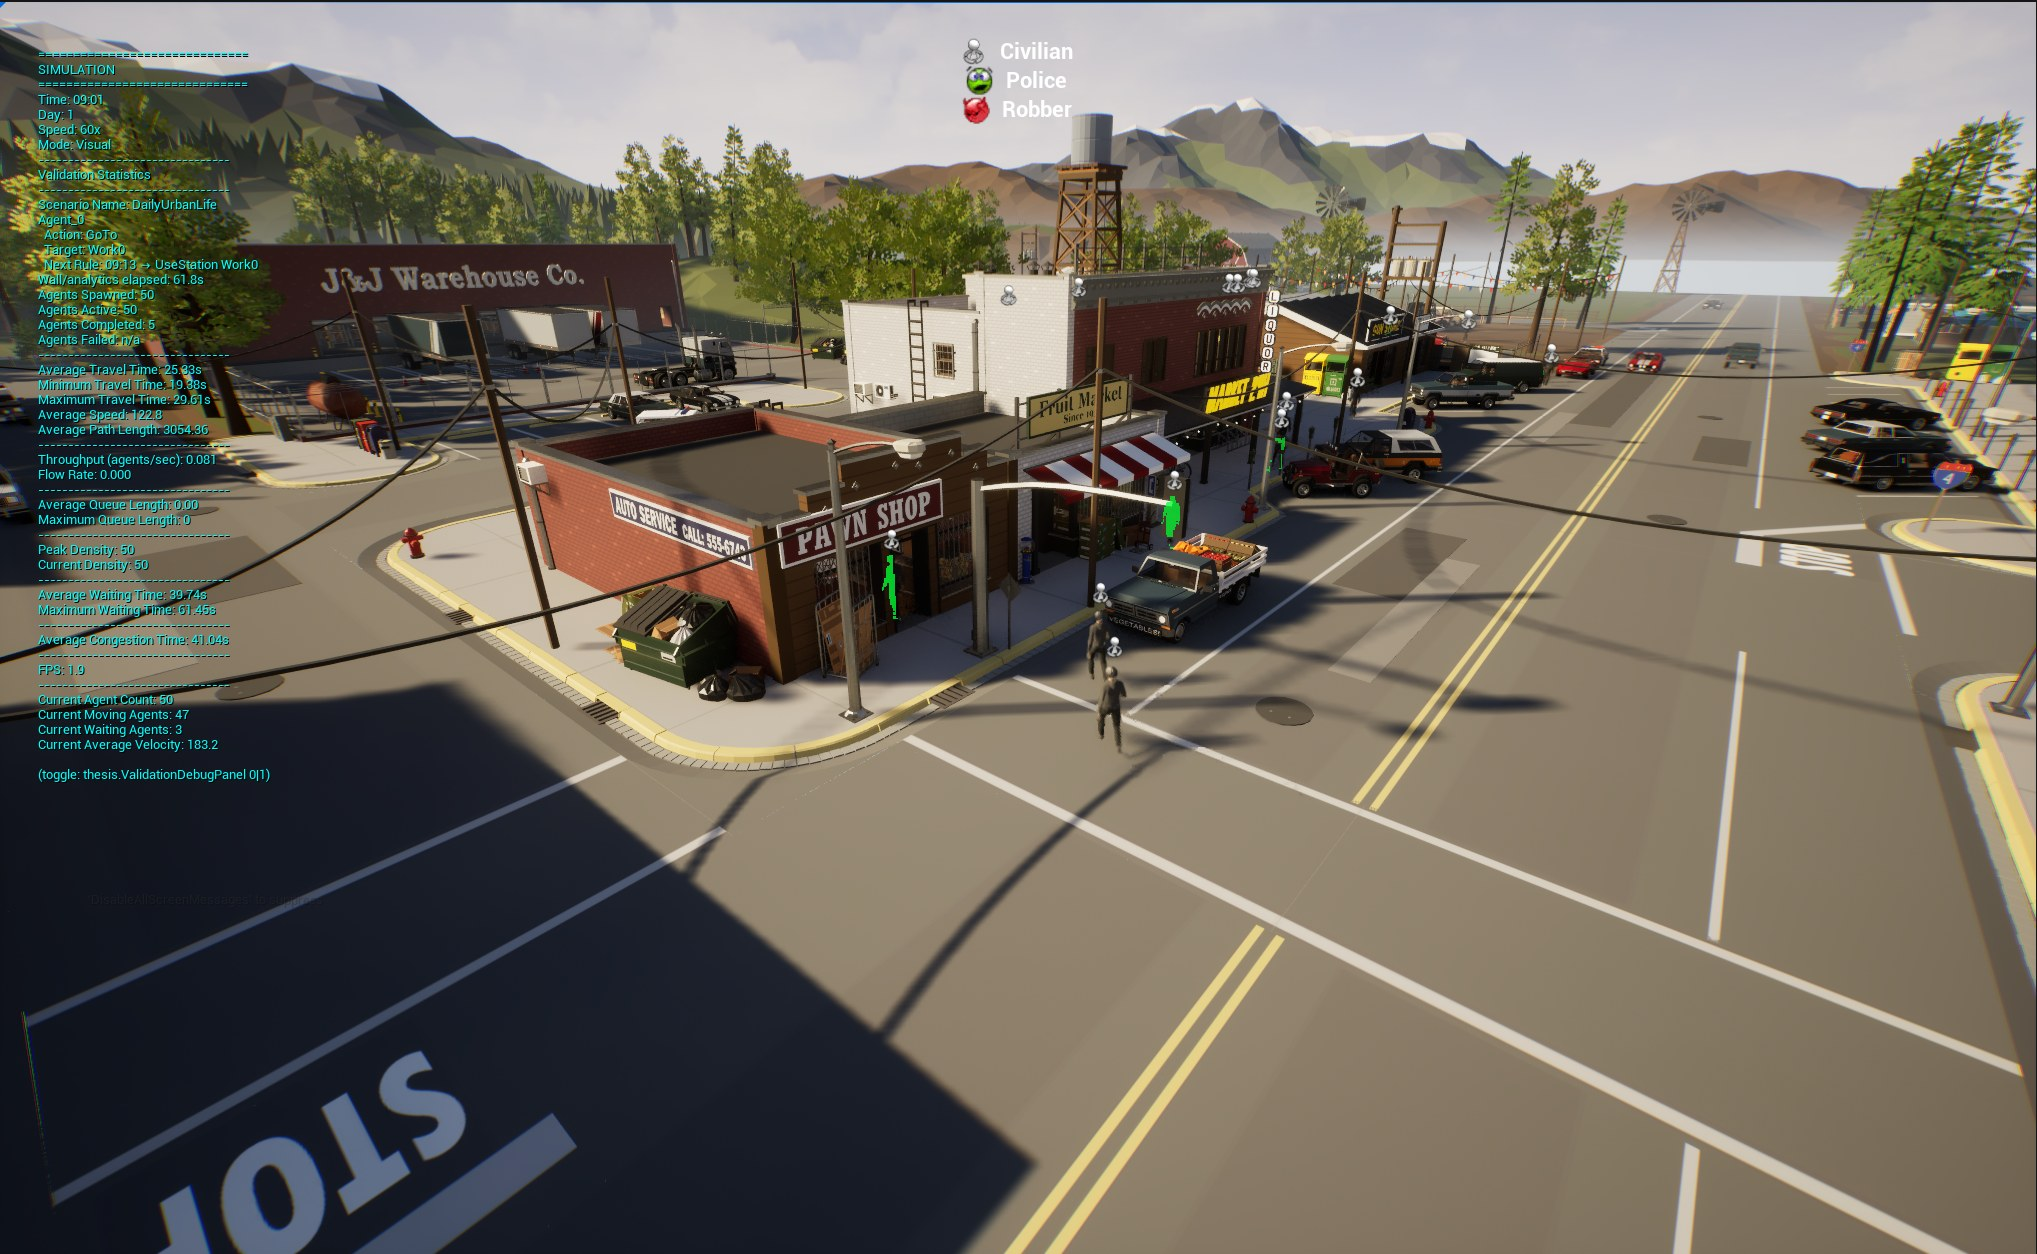
\includegraphics[width=0.85\textwidth]{images/shots/dul_overview.jpg}
\caption[Daily Urban Life map during the morning]{Daily Urban Life map during the morning in Visual mode, where each figure is a person following their own schedule and the validation panel is on the left.}
\label{fig:app-dul-overview}
\end{figure}

\begin{table}[H]
\centering
\small
\begin{tabular}{|l|c|}
\hline
\rowcolor{headgray}\textbf{Outcome} & \textbf{\shortstack{Percent of the authored\\rules, walks or visits}} \\
\hline
\tabinput{analysis/tables/dul_rows.tex}
\end{tabular}
\caption[Daily Urban Life outcomes]{Daily Urban Life outcomes with 50 people as a share of the authored rules, of the walks or of the station visits (mean of five runs).}
\label{tab:app-dul}
\end{table}

The schedule leaves enough time for walking, as \texttt{Agent\_0} has 18 simulated minutes between leaving for \texttt{Work0} and sitting at their desk, and the walk is about 150~m long. Two things delay rules: competition at shared places and long walks to crowded target points. Two shifts share 25 desks, and of the 481 desk requests in the five runs, 260 queued and 300 ended in a completed work session, and these counts overlap because a request that queued can still end in a completed session. The wait per station visit averaged 1.7 simulated minutes, and queueing was 34\% of the start delay of station rules (\cref{fig:app-start-delay}). A desk queue can outlast the time until the person's break, and since the break releases the place as designed, 7 to 32 reserved stations per run were left before the person reached them. The scenario therefore measures competition for work sessions, which the time scale of Visual mode had hidden, because there a walk took longer than the schedule allowed for it.

Single-point targets still take time (\cref{fig:app-dul-arrivals}), as 75\% of the walks to \texttt{Work3} arrived, against 90 to 100\% at the other work areas. The median walk to a work area took 1.6 simulated minutes, close to the 1.3 minutes that 150~m at 2~m/s needs, but the walks to these shared single points have a long tail. Of the 235 walks that arrived, 43 took more than 5 minutes while the person milled about a crowded point, and 7 of them, like all 15 walks that failed, lasted until the GoTo time-out. A person who keeps being pushed around near a crowded point without coming to rest, or who rests just outside the arrival radius, ends their walk only at that time-out. The walk then counts as arrived if the person is within 180~cm and as failed otherwise, and the time-out lasts 180 real seconds, which Accurate mode does not convert and which the clock counts as 90 simulated minutes. These long walks raise the mean walk to a work area to 7.5 simulated minutes, and these walks account for 95\% of the late minutes. Without the 7 walks that ended on the time-out, the mean is 5.0 minutes, so the time-out adds about a third to the mean, while crowding at the single points causes the rest of the tail. A few people never left home, because no sidewalk path started where they stood, and overall, 94\% of walks counted as arrived, an upper bound by the definition of \cref{sub:app-recording}.

\begin{figure}[H]
\centering
\begin{tikzpicture}
\begin{axis}[
  width=0.95\textwidth, height=5.6cm,
  ybar=3pt, bar width=14pt, ymin=0, ymax=112,
  ytick={0,25,50,75,100},
  symbolic x coords={Work0,Work1,Work2,Work3,Work4,Work5,Work6}, xtick=data,
  ylabel={Walks that arrived (\%)}, xlabel={Work area},
  % axis lines resets the enlargement, so enlarge x limits must follow it
  axis lines=left, enlarge x limits=0.08, ymajorgrids, grid style={black!12},
  tick label style={font=\small}, label style={font=\small},
  /pgf/number format/assume math mode=true,
  nodes near coords, every node near coord/.append style={font=\footnotesize, inner sep=1.5pt}]
\addplot[fill=cBlue, draw=cBlue!70!black] table[x=area, y=accurate] {analysis/data/dul_work_arrivals.dat};
\end{axis}
\end{tikzpicture}
\caption[Walks that arrived at each work area]{Share of walks that arrived at each work area (five runs).}
\label{fig:app-dul-arrivals}
\end{figure}

\section{Shopping Center: Mall A and Mall B}
\label{sec:app-mall}

\label{sub:app-mall-authored}

Each shopping center has its own schedule for ten people: 53 rules in Mall A, of which 28 are \texttt{MoveTo}, 15 \texttt{UseStation} and 10 \texttt{Idle}, and 59 in Mall B, which adds four walks, one station use and the single \texttt{Interact}. Every person waits at an entrance, browses one or two shops, uses a shop desk or a seat, eats, and leaves. In Mall A, nine people eat, and the meal is a two-stage pipeline: a food counter for 10 minutes, then a food table for 14 (\cref{lst:malla-pipeline} in \cref{chap:contribution}). The table is chosen only when the counter stage ends, so a slow counter delays the table request. \Cref{fig:app-malla} shows the entrance of Mall A and its levels, as the map has more than one floor.

\begin{figure}[H]
\centering
\begin{subfigure}[b]{0.32\textwidth}\centering
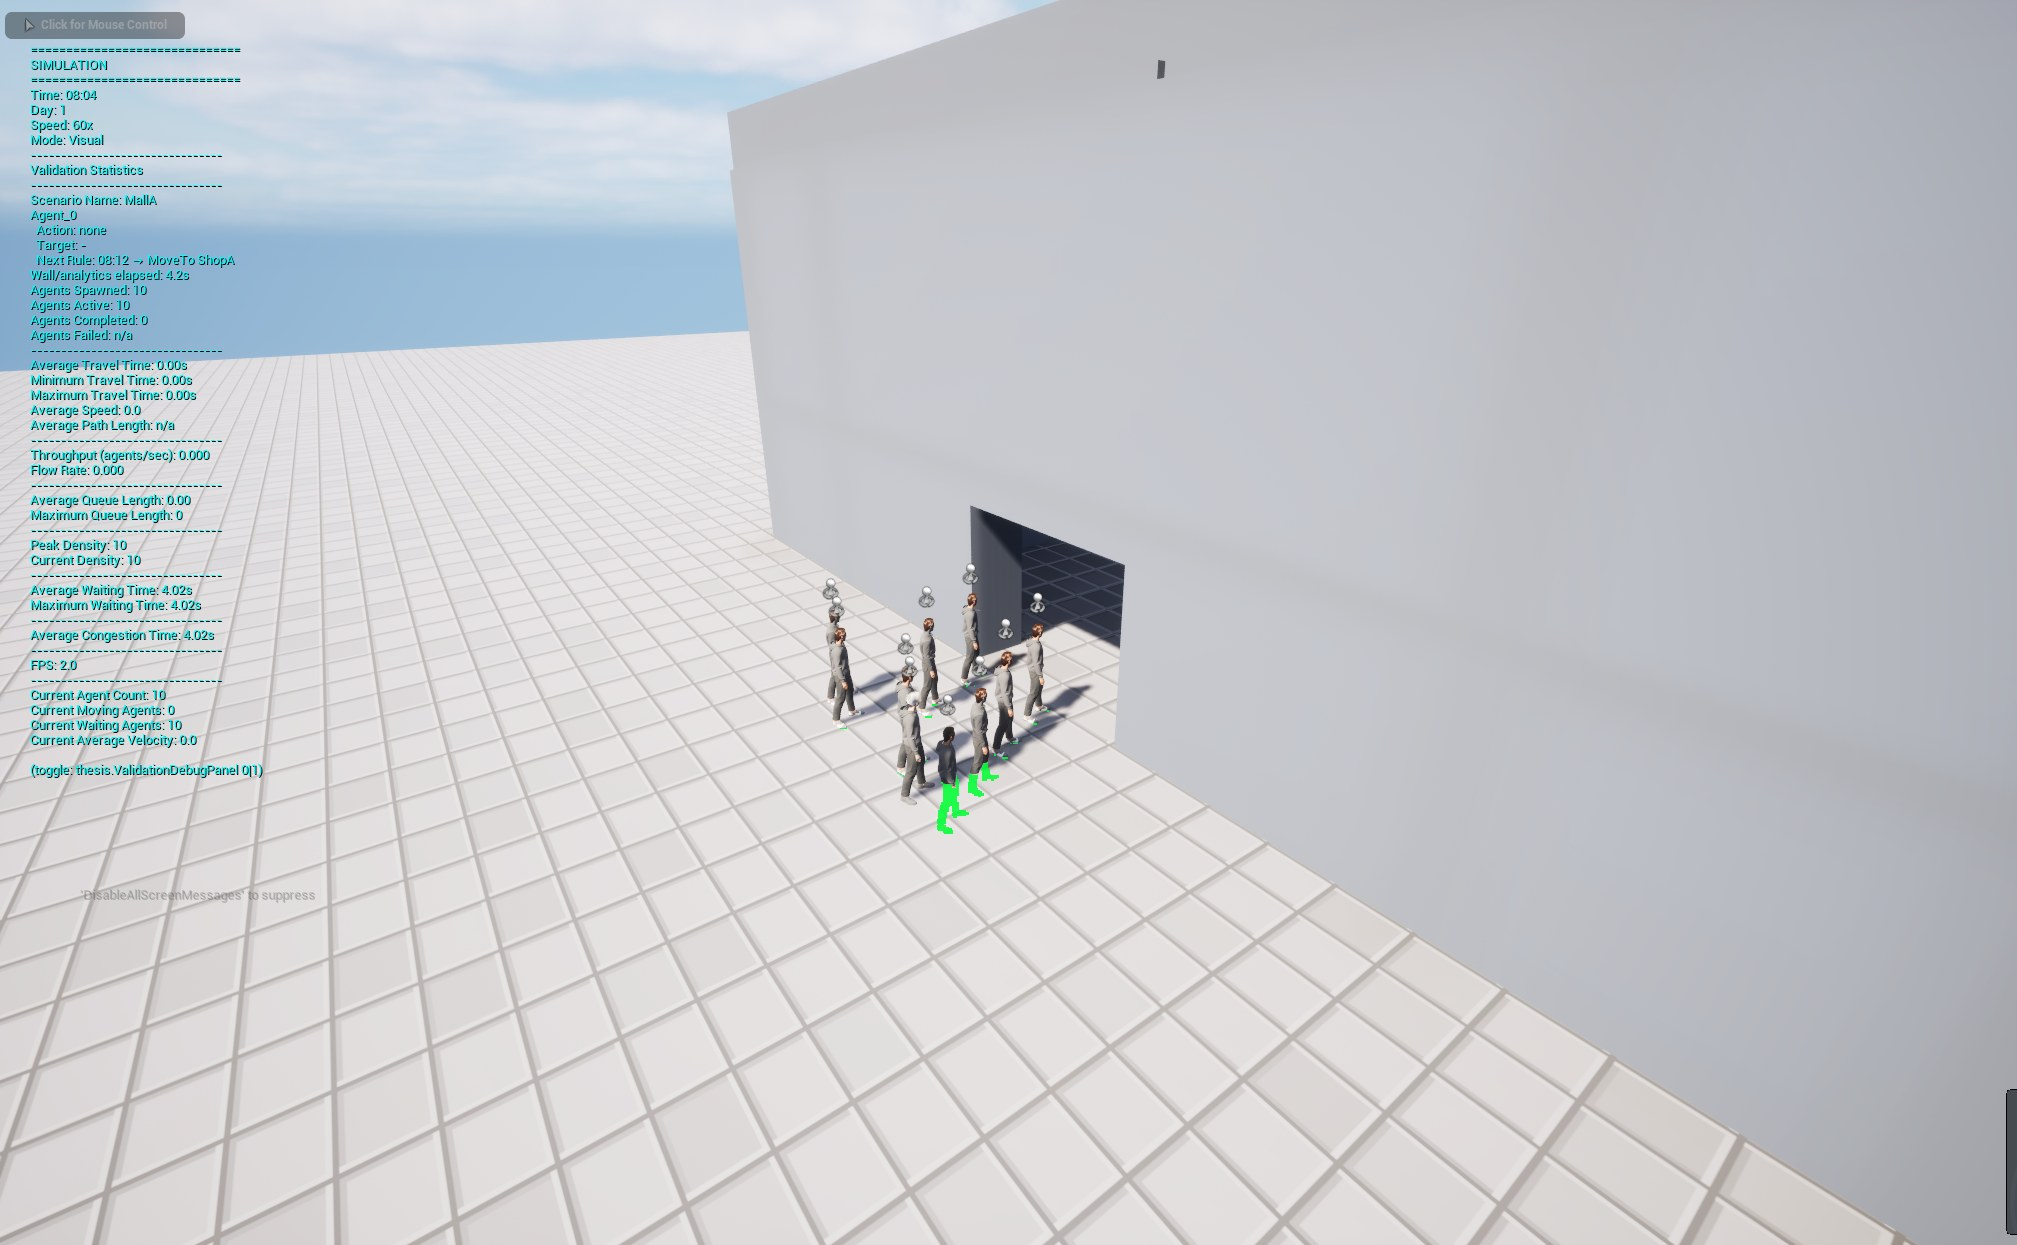
\includegraphics[width=\linewidth]{images/shots/malla_entrance.jpg}
\caption{The entrance}
\end{subfigure}\hfill
\begin{subfigure}[b]{0.32\textwidth}\centering
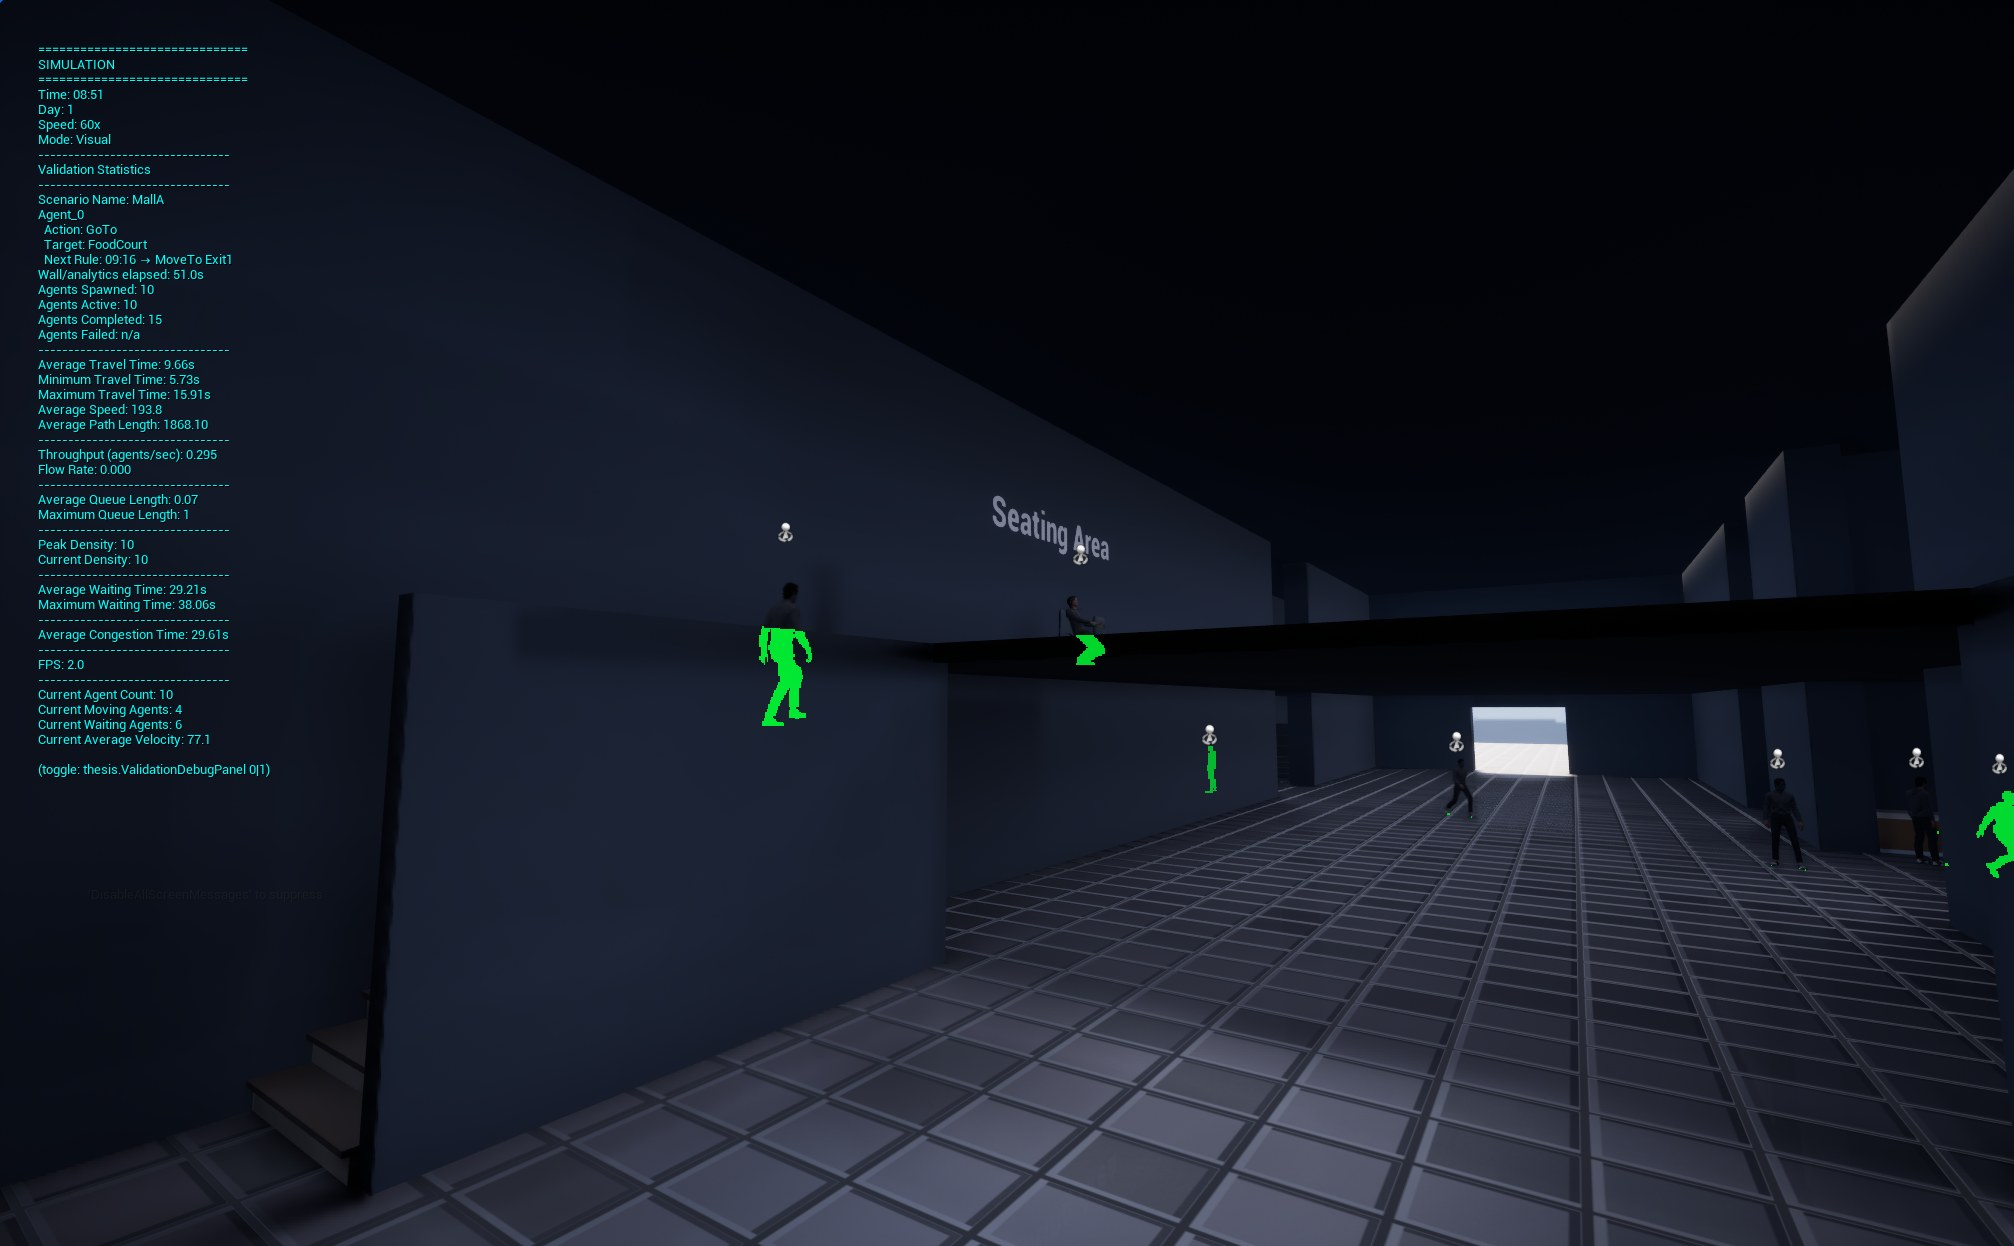
\includegraphics[width=\linewidth]{images/shots/malla_upper_level.jpg}
\caption{Its levels}
\end{subfigure}\hfill
\begin{subfigure}[b]{0.32\textwidth}\centering
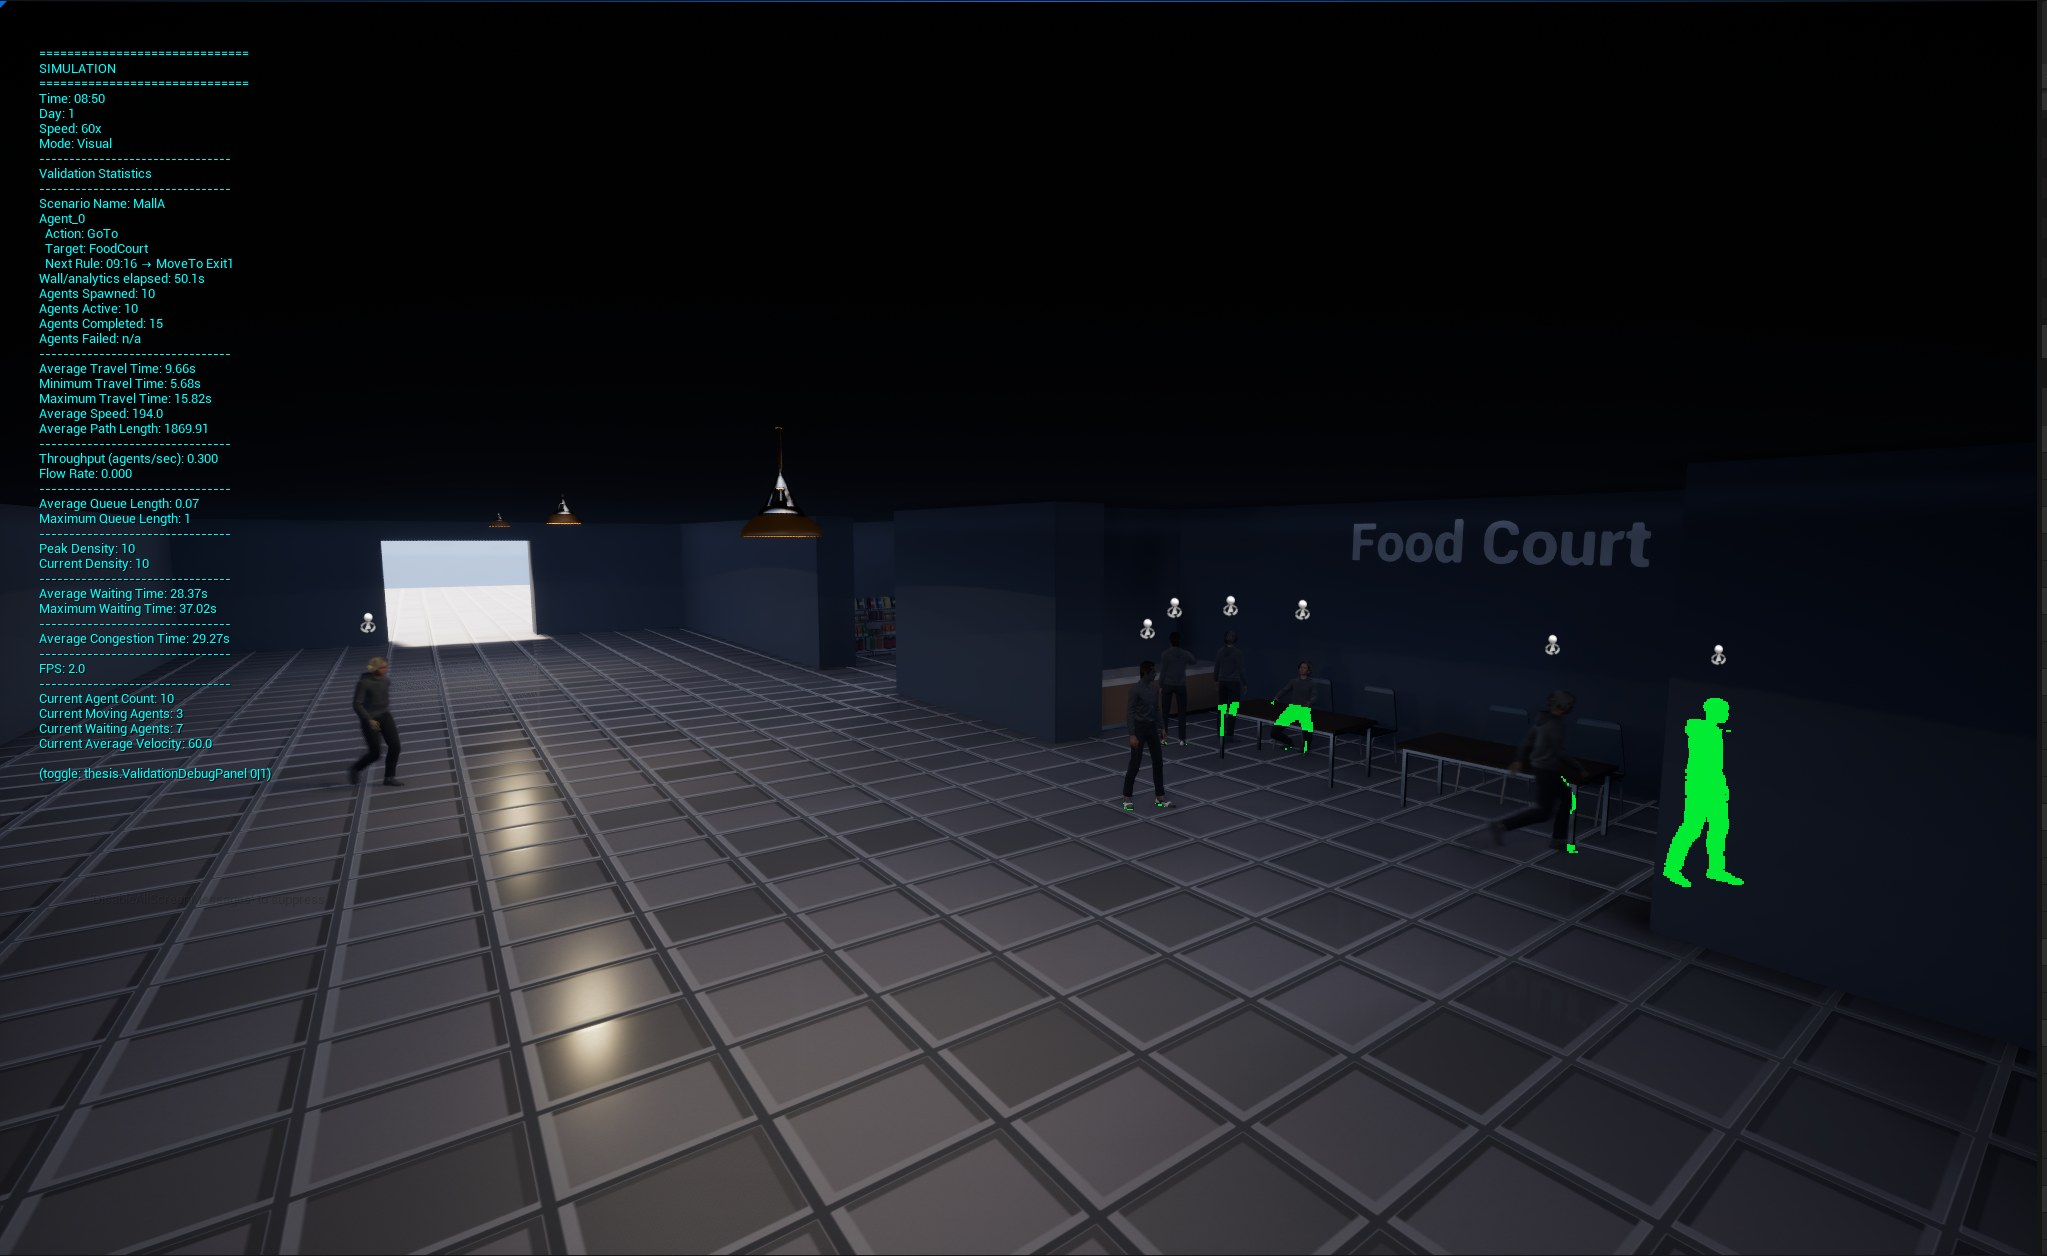
\includegraphics[width=\linewidth]{images/shots/malla_foodcourt.jpg}
\caption{The food court}\label{fig:app-malla-food}
\end{subfigure}
\caption[Mall A]{Mall A, with (a) its entrance, (b) a view of its levels and (c) its food court, where a meal uses a counter and then a table.}
\label{fig:app-malla}
\end{figure}

Mall B keeps the same ten people and their schedules with three changes: four people eat at a second food court, service points have two places instead of one, and \texttt{Agent\_0} first walks to a button (\texttt{MoveTo} at 08:04) and presses it (\texttt{Interact} at 08:08). The button opens a second entrance, where the odd-numbered people start (\cref{fig:app-mallb}).

\begin{figure}[H]
\centering
\begin{subfigure}[b]{0.32\textwidth}\centering
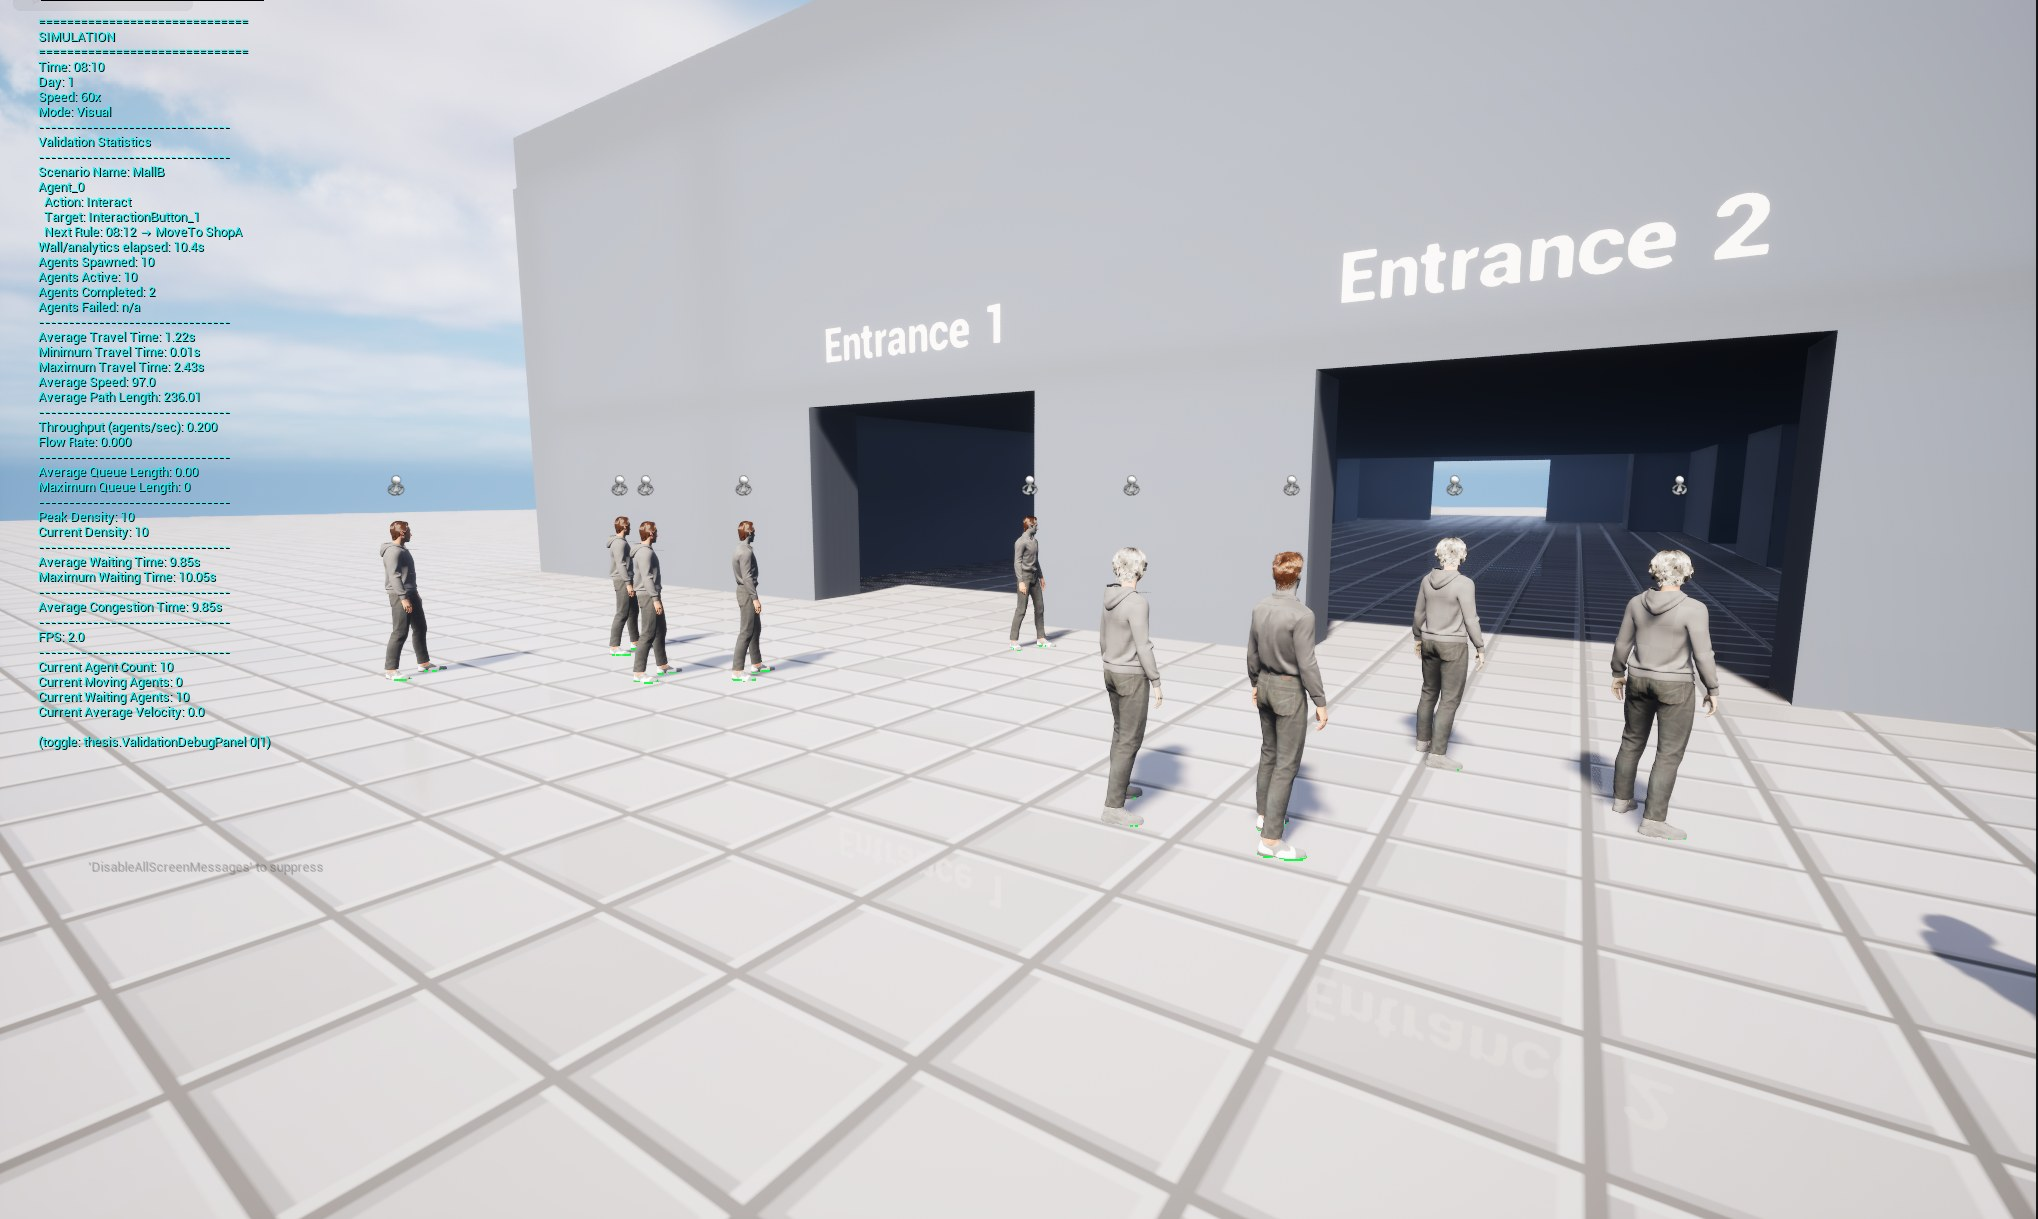
\includegraphics[width=\linewidth]{images/shots/mallb_entrances.jpg}
\caption{The two entrances}
\end{subfigure}\hfill
\begin{subfigure}[b]{0.32\textwidth}\centering
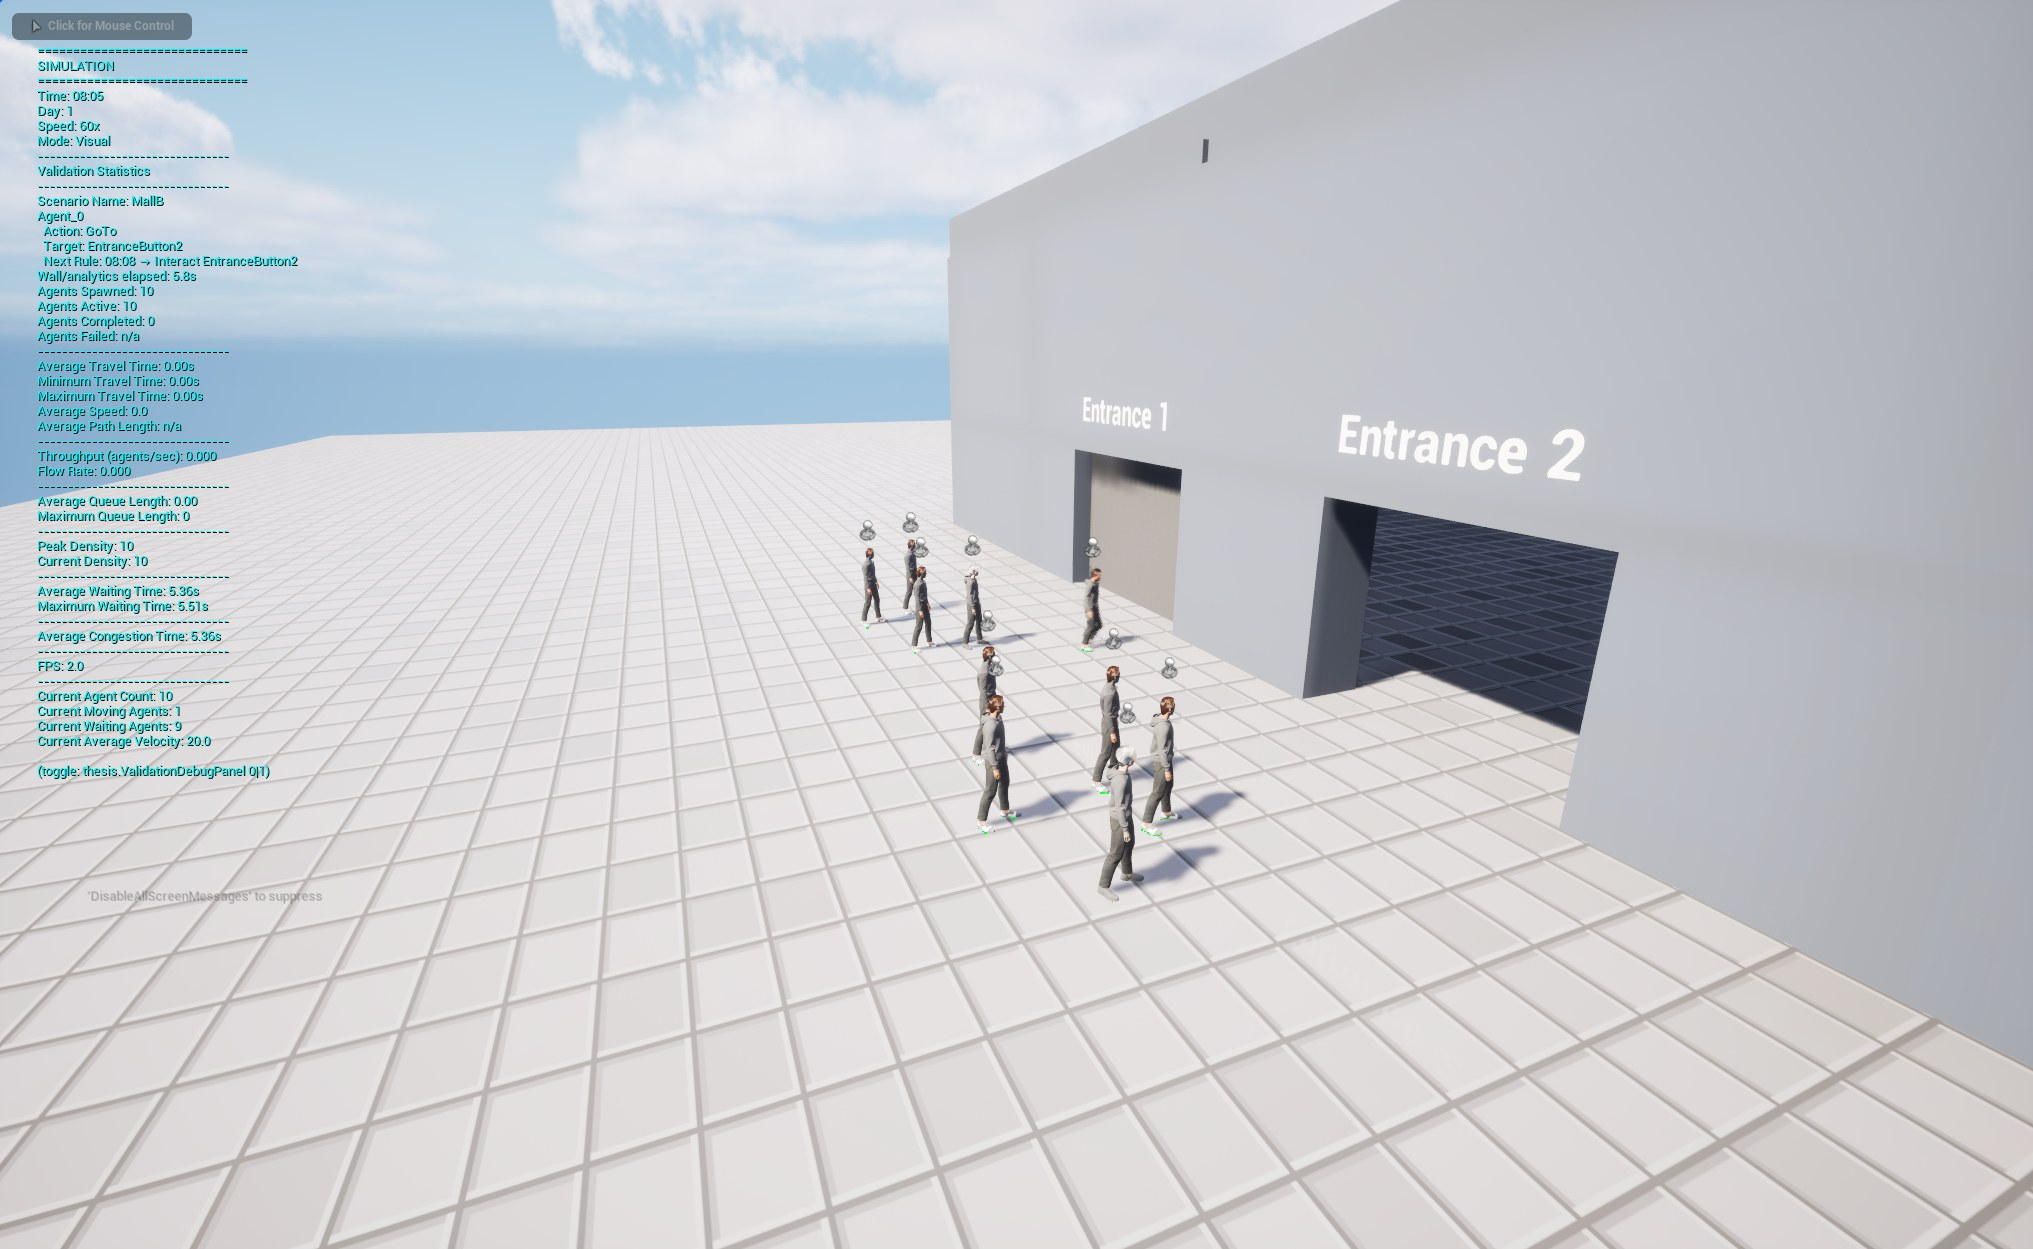
\includegraphics[width=\linewidth]{images/shots/mallb_interact.jpg}
\caption{Walking to the button}
\end{subfigure}\hfill
\begin{subfigure}[b]{0.32\textwidth}\centering
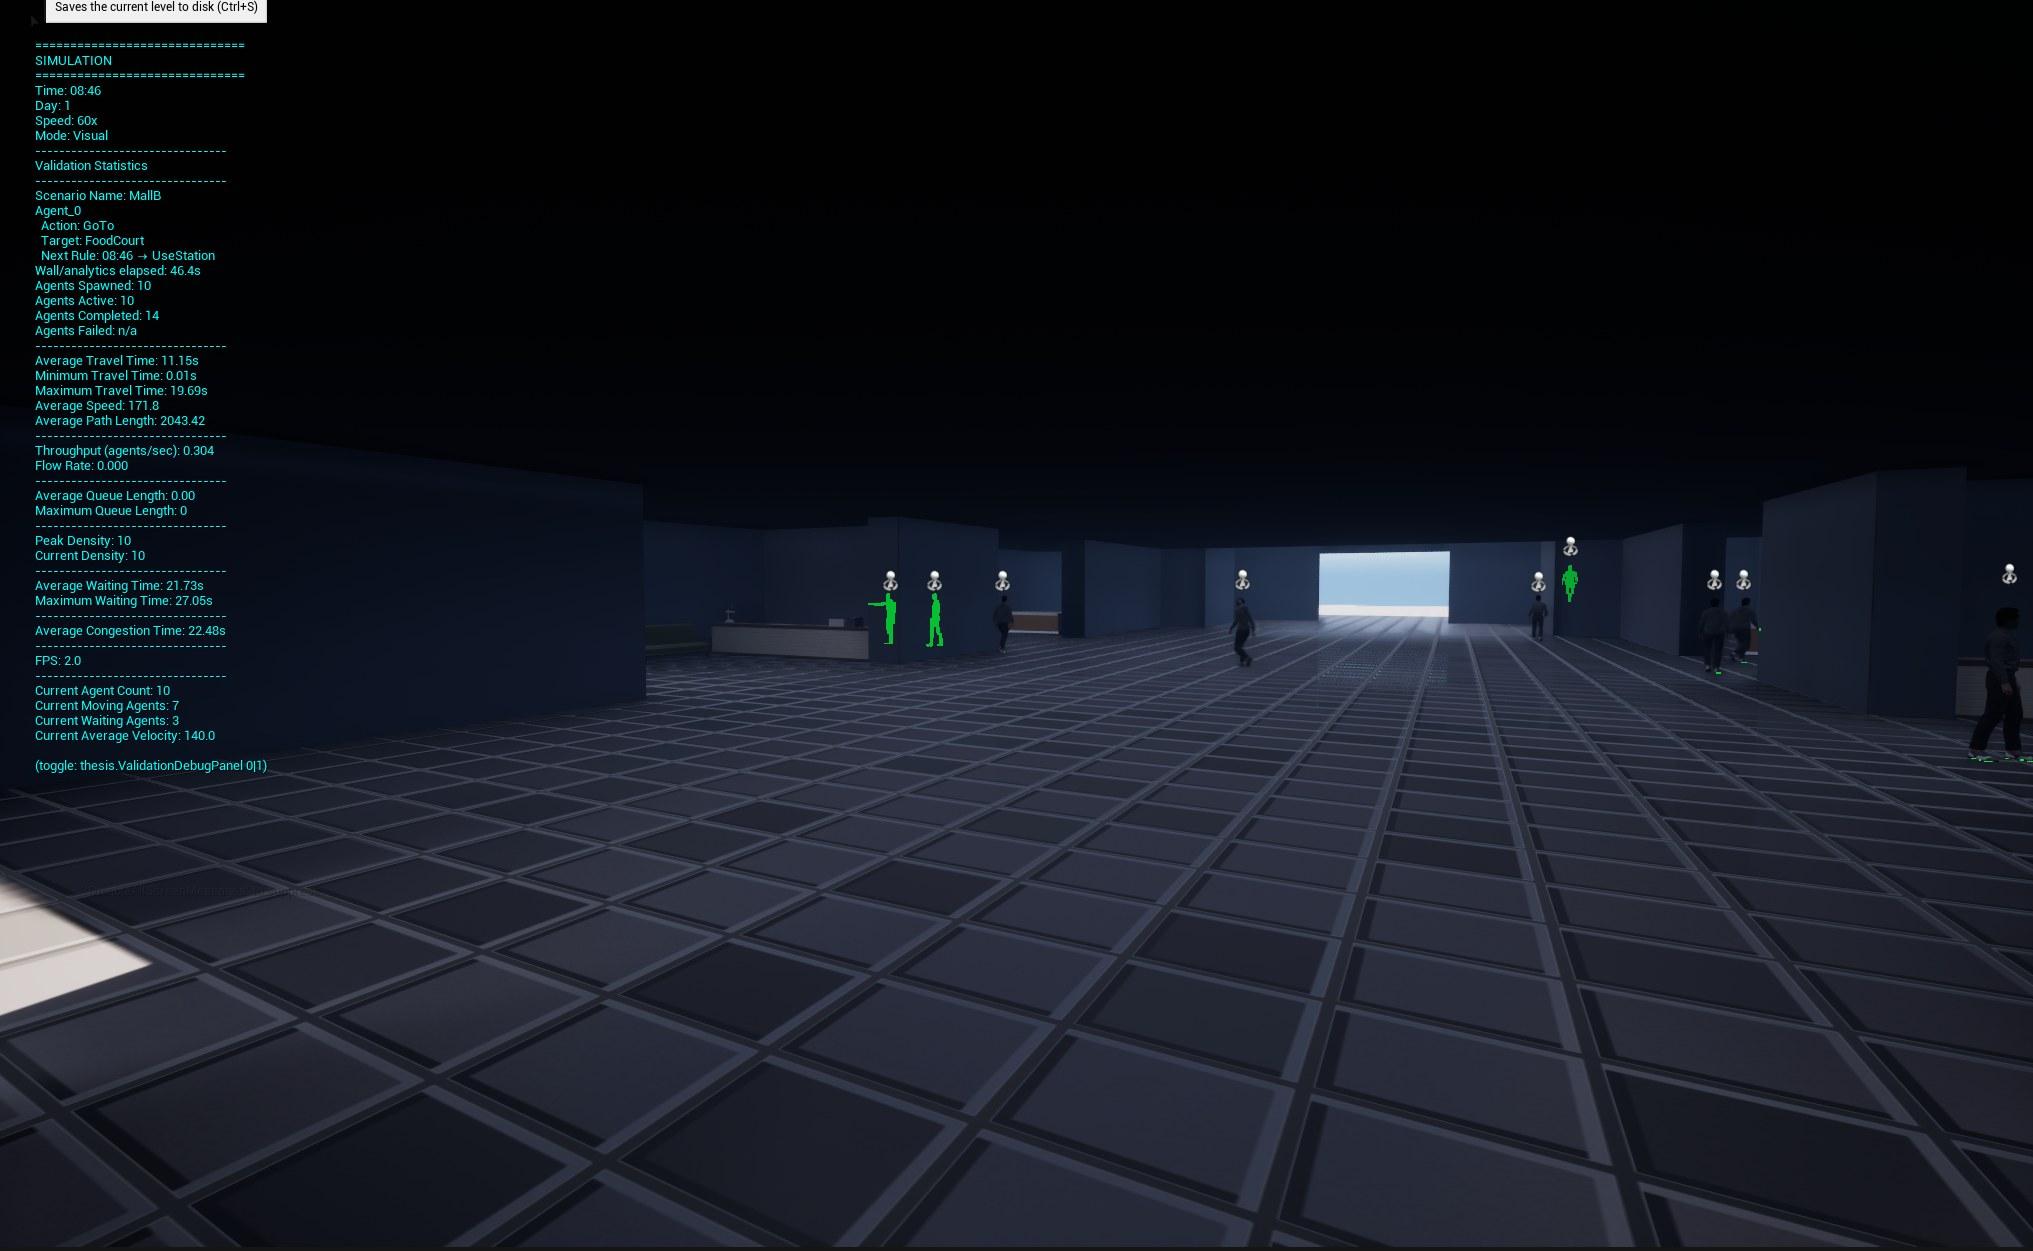
\includegraphics[width=\linewidth]{images/shots/mallb_interior.jpg}
\caption{The interior}
\end{subfigure}
\caption[Mall B]{Mall B, with (a) its two entrances, (b) a person walking to the button that opens the closed entrance with the \texttt{Interact} action, and (c) its interior.}
\label{fig:app-mallb}
\end{figure}

Both maps have two shops with desks, a seating area, and a food court built as a super station with four counters and four tables (\cref{fig:app-malla-food}). Mall B adds \texttt{FoodCourt2}, the button, and a gate that removes its area from the navigation mesh while closed. The infrastructure manager places people at the entrances and sets the capacity of every station whose actor tag or identifier matches a configured name, so that the capacity tests can change one kind of station at a time. A place is reserved when the rule fires, and a person who finds every station of the requested type full joins the queue of the first one and waits where they stand. The walk to the food court took 0.4 simulated minutes on average in Mall A, well within the 10 minutes that \texttt{Agent\_0}'s schedule allows.

\subsection{Capacity experiments}
\label{sub:app-mall-capacity}

We kept the Mall A map and schedule fixed and changed one kind of station at a time (shop desks, counters or tables) to one, two or three places, with five runs per setting, later extended to 30 runs per setting (\cref{fig:app-capacity}). In the counter and table tests, the shop desks kept their editor capacity, which allowed two people at one desk, so the one-place bars of the three groups are not the same configuration, although their medians coincide.

\begin{figure}[H]
\centering
\begin{tikzpicture}
\begin{axis}[
  width=0.9\textwidth, height=5.8cm,
  ybar=3pt, bar width=18pt, ymin=0, ymax=1.65,
  ytick={0,0.5,1,1.5},
  symbolic x coords={1,2,3}, xtick=data, xticklabels={One place, Two places, Three places},
  ylabel={Median wait per visit (min)},
  axis lines=left, ymajorgrids, grid style={black!12},
  tick label style={font=\small}, label style={font=\small},
  /pgf/number format/assume math mode=true,
  enlarge x limits=0.22, legend image code/.code={\draw[#1] (0cm,-0.08cm) rectangle (0.3cm,0.14cm);},
  legend style={draw=none, fill=none, at={(0.5,1.02)}, anchor=south, legend columns=3, font=\small, /tikz/every even column/.append style={column sep=10pt}},
  nodes near coords, every node near coord/.append style={font=\scriptsize, inner sep=1.5pt, /pgf/number format/fixed, /pgf/number format/precision=2}]
\addplot[fill=cSky, draw=cSky!60!black] table[x=places, y=desks] {analysis/data/capacity30_median.dat};
\addlegendentry{Shop desks changed}
\addplot[fill=cOrange, draw=cOrange!60!black] table[x=places, y=counters] {analysis/data/capacity30_median.dat};
\addlegendentry{Food counters changed}
\addplot[fill=cGreen, draw=cGreen!60!black] table[x=places, y=tables] {analysis/data/capacity30_median.dat};
\addlegendentry{Food tables changed}
\end{axis}
\end{tikzpicture}
\caption[Median wait per visit by number of places]{Median wait per station visit in Mall A by number of places (simulated minutes, 30 runs per setting, lower is better), with the full statistics in \cref{tab:app-capacity}.}
\label{fig:app-capacity}
\end{figure}

The one-place baseline differs between the two rounds, at 0.81 simulated minutes over the five seeds and 0.84 over the 30 runs, so each value below is quoted with the round it comes from. In the first five runs per setting, two or three places at the tables lowered the wait per visit from 0.81 to 0.51 simulated minutes in all five runs ($p=0.008$). More places at the counters raised it to 1.21 with two places ($p=0.008$) and 1.35 with three ($p=0.10$), and the queue joins explain why. With one place per counter, 10 counter requests and 5 table requests queued over the five runs. With two or three counter places, the counter queues disappeared, but more diners reached the tables at the same time, and as the tables kept one place each, 10 and 11 table requests queued, so the bottleneck moved down the pipeline and the wait grew. With one table place, only 5 of 45 table requests queued in five runs, about one queued visit per run, so the lower wait with more table places is the removal of that visit. No person ever joined a desk queue, and the desk settings made no difference ($p=1.0$). Over 30 runs per setting (\cref{fig:app-capacity,tab:app-capacity}), the medians show the same pattern: 0.84 minutes with one place, 1.34 and 1.26 with two and three counter places ($p<0.001$), 0.51 with two or three table places ($p<0.001$) and 0.84 for every desk setting ($p=0.89$). The table result is a difference of about 20 seconds per visit, small against a 24-minute meal, so what matters is its direction, which behaves as a tandem queue should and which the lunch rush below repeats with waits of several minutes. The mean with three counter places (2.43 minutes) is not a valid summary, because in 3 of its 30 runs a diner was admitted to a table they never reached and held it until the run ended, with one or two people queued behind them. These runs averaged 7.5 to 16.0 minutes of wait per visit, while the other 27 runs averaged 1.25 minutes (\cref{sub:app-edge-cases}).

The logs also explain why queues persist while equivalent stations are free. All queue joins of a given kind went to a single station, because a queued person stays with the first matching station even when an equivalent one frees up. The capacity comparisons therefore hold under this selection policy, and one shared queue per area could change their sizes. A place is also held while its owner walks to it, though briefly at the real walking pace: in Mall A, a person reserved a counter on average 0.3 minutes and a seat 0.6 minutes before reaching it.

\subsection{A lunch rush}
\label{sub:app-mall-rush}

Ten people seldom compete, so we also ran a lunch-rush variant of the Mall A schedule, with ten runs per setting (\cref{tab:app-rush}). In this variant, the schedule sends all nine diners to the food court at 08:40 and has them request a counter at 08:50, they leave no earlier than 09:20, and the other rules are unchanged. We did not add people by copying them, because with 50 copies of the authored schedule the shared single-point targets jammed. In five such runs, only 26 to 77 of 87 to 107 walks arrived, 148 to 200 of the 265 rules were dispatched and 11 to 41 station services were completed.

\begin{table}[H]
\centering
\footnotesize\setlength{\tabcolsep}{3pt}
\begin{tabular}{|l|c|c|c|c|c|c|c|c|}
\hline
\rowcolor{headgray}\textbf{Stations changed} & \textbf{Places} & \textbf{\shortstack{Median\\wait}} & \textbf{\shortstack{Range\\over runs}} & \textbf{\shortstack{Mean wait\\(SD)}} & \textbf{\shortstack{Queued visits\\per run}} & \textbf{\shortstack{Start\\delay}} & \textbf{\shortstack{Start delay spent\\queueing (\%)}} & \textbf{$p$} \\
\hline
\tabinput{analysis/tables/rush_rows.tex}
\end{tabular}
\caption[Mall A during a lunch rush]{Wait per station visit and start delay in Mall A during a lunch rush with ten runs per setting, in simulated minutes, where SD is the standard deviation and $p$ compares three places with one, and where the start delay covers the counter stage only, so a queue that moved to the tables appears in the wait per visit and not in that column.}
\label{tab:app-rush}
\end{table}

In every rush run, one of the nine diners could not get within the arrival radius of the crowded food-court point, and their walk timed out before it reached the counter stage, so a run records eight counter requests rather than nine and each setting 80 over its ten runs. With one place per counter, 39 of the 80 counter requests queued, the wait per visit averaged 4.6 simulated minutes (median 4.8), and queueing was 92\% of the start delay of station rules. Three places per counter removed the counter queues but moved them to the tables, which kept one place: 40 of 80 table requests queued, later pipeline stages queued for 14.9 minutes on average, and the wait per visit rose to 8.6 minutes (median 5.9, $p<0.001$). Three places per table lowered the wait only slightly (4.4 minutes, median 4.6, $p=0.002$), because the counters, which kept their editor capacity in the table tests, stayed the bottleneck, with 39 of 80 counter requests queued and none at the tables. Under contention, extra places at one stage of the pipeline moved the queue to the next stage that was short of capacity.

\subsection{Where late minutes come from}
\label{sub:app-mall-late}

Late starts were rare, as between 0\% and 4\% of the dispatched rules started late in the capacity settings, and the few late minutes in Mall A were mostly spent finishing a previous activity rather than walking. Lateness stops at dispatch, however, so \cref{fig:app-start-delay} also splits the whole start delay of station rules. In Mall A, a station rule started its service on average 1.0 simulated minute after it became eligible, with no lateness, 0.7 minutes queueing for a place and 0.3 minutes walking to the reserved station. Queueing was 67\% of the start delay over all 50 Mall A runs and 76\% in Mall A as authored, and later pipeline stages, such as the table after the counter, queued for 1.2 minutes on average. The start delay covers only the first stage of a pipeline, so with two or three counter places it shows no queueing, while the table stage queued for 3.2 to 3.6 minutes on average. The 105 Daily Urban Life station rules that never started are also left out of its mean, and in Mall B, where no person queued, the start delay was the walk alone. With walking at its real pace, waiting for shared stations is the largest part of the gap between authored and realized times in the shopping centers, while in Daily Urban Life long walks to crowded target points take a larger share (\cref{sub:app-dul-results}).

\begin{figure}[H]
\centering
\begin{tikzpicture}
\begin{axis}[
  width=0.9\textwidth, height=5cm,
  xbar stacked, bar width=14pt, xmin=0, xmax=6,
  ytick={0,1,2}, yticklabels={Mall A, Mall B, Daily Urban Life}, y dir=reverse,
  xlabel={Mean start delay of a station rule (min)},
  axis lines=left, xmajorgrids, grid style={black!12},
  tick label style={font=\small}, label style={font=\small},
  /pgf/number format/assume math mode=true,
  enlarge y limits=0.35, legend image code/.code={\draw[#1] (0cm,-0.08cm) rectangle (0.3cm,0.14cm);},
  legend style={draw=none, fill=none, at={(0.5,1.03)}, anchor=south, legend columns=4, font=\small, /tikz/every even column/.append style={column sep=8pt}}]
\addplot[fill=cPurple, draw=cPurple!60!black] table[y=y, x=lateness] {analysis/data/start_delay_split.dat};
\addlegendentry{Lateness $\ell$}
\addplot[fill=cVerm, draw=cVerm!60!black] table[y=y, x=queue] {analysis/data/start_delay_split.dat};
\addlegendentry{Queueing $q$}
\addplot[fill=cBlue, draw=cBlue!60!black] table[y=y, x=walk] {analysis/data/start_delay_split.dat};
\addlegendentry{Walking $w$}
\addplot[fill=cOrange, draw=cOrange!60!black] table[y=y, x=position] {analysis/data/start_delay_split.dat};
\addlegendentry{Positioning $p$}
\end{axis}
\end{tikzpicture}
\caption[Start delay of station rules]{Start delay of station rules split into its parts (simulated minutes), with the values in \cref{tab:app-start-delay}.}
\label{fig:app-start-delay}
\end{figure}

\subsection{Mall A against Mall B}
\label{sub:app-mall-layouts}

In Mall B, no person ever queued, and its rules started on time about as often as in Mall A, but because schedule, layout and capacities all differ, the comparison does not isolate the effect of layout. In Visual mode, these runs had exposed an edge case of the reservations, as a reservation has no time-out and a failed path only stops the person, so a person who never reached their reserved station held the place until the run ended. In Accurate mode, no station visit was still open at the end of any layout run, and no walk failed, so this edge case did not affect this comparison. It can still occur, and it dominated three capacity runs with three counter places (\cref{sub:app-mall-capacity}), in which a person admitted to a table never reached it.

\section{Emergency Evacuation}
\label{sec:app-evac}

\label{sub:app-evac-authored}

The evacuation needs one rule (\cref{lst:app-evac}), and the rest is scenario code. The emergency manager starts a fire incident covering the map, raises the alarm for every person and starts a countdown authored as 120 seconds, which keeps its Visual meaning of 120 simulated minutes in Accurate mode. Each person first waits for a reaction delay, authored as 0 to 5 seconds, which Accurate mode turns into 0 to 5 simulated minutes, long for a reaction to an alarm but short against the 120-minute countdown. The person then chooses an exit by a score that combines distance and queue length, asks for a queue place and walks to their slot, and may switch exits every 5 seconds, at most three times.

\begin{lstlisting}[language=XML, caption={The evacuation schedule. The trigger is global and idempotent, so one coordinator is enough.}, label={lst:app-evac}]
<agent id="Agent_0">
  <rule time="08:05"><then action="StartEvacuation"/></rule>
</agent>
\end{lstlisting}

The map is an open floor with walls, two exits, and a safe zone (\cref{fig:app-evac-exits}). Each exit lets one person through every 1.5 real seconds, a constant that Accurate mode does not convert, so an exit serves one person every 45 simulated seconds, far fewer than a real door of that width would pass. The results below therefore test the exit and queue mechanism rather than an evacuation time, and they cannot yet say whether an exit would become a choke point, the question that \cref{chap:intro} opens with. Each exit lays out its queue as slots behind it, at most 25 on this map (the recorded peak at both exits in every run with 100 or 200 people). A person who has passed an exit walks to the safe zone and is counted as safe within 200~cm of its center, and when the countdown ends, every other person becomes a casualty.

\label{sub:app-evac-results}

We ran the evacuation with 50, 100, and 200 people, three times each, made the larger populations by copying the map's people, and repeated every run with a step of 0.25 instead of one simulated second per frame (\cref{fig:app-evac}). At one second per frame, all 50 people passed an exit before the countdown ended, 89 to 100 of 100, and 44 to 75 of 200. At 0.25 seconds per frame, all 50 and all 100 did so in every run, and 57 to 66 of 200.

An exit lets one person through every 45 simulated seconds, so in the 120-minute countdown it could pass 160 people, and two exits 320, but the exits passed at most 51 people each, so their designed capacity does not explain the losses. The losses came from stalled exits: in one run with 100 people and one with 200 at one-second steps, one exit passed at most two people after its queue stalled, and with 200 people both exits passed fewer than 40 at either step. We did not check the positions of the people, but the pattern suggests an edge case of the exit queues. People who cannot get a queue place keep pressing towards the exits, so the person who becomes first in a queue cannot always reach the head slot. Only 10 to 31 people per run were counted as safe, because the first arrivals stop at the rim of the safe zone and the rest cannot enter. Everyone else counts as a casualty, including people who had left the building, so we report passing an exit rather than casualties, and we treat the stalled exits and the blocked safe zone as edge cases of the scenario (\cref{sub:app-edge-cases}, per-run counts in \cref{tab:res-evac-runs}).

\begin{figure}[H]
\centering
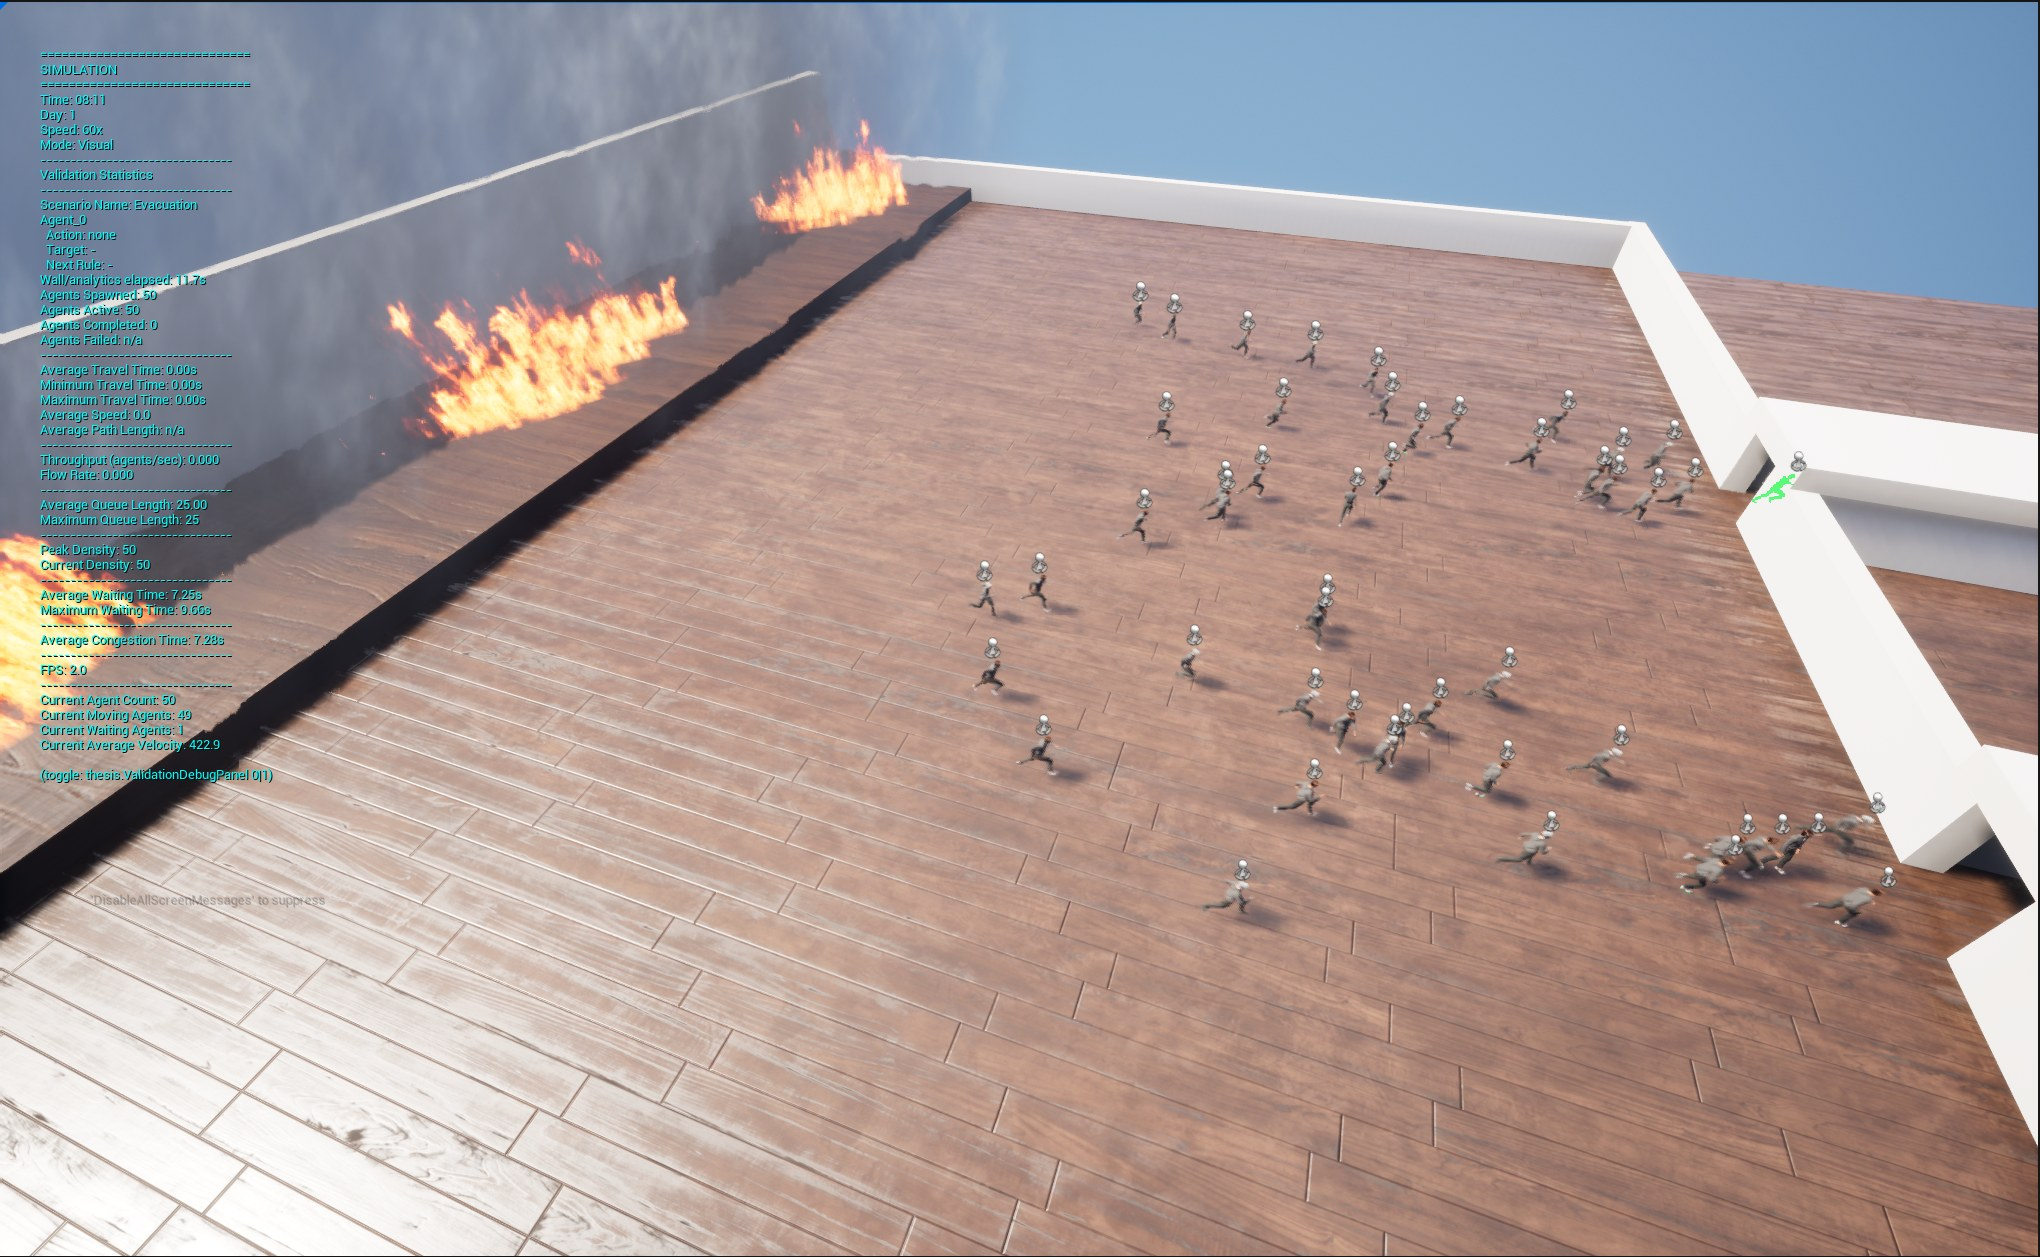
\includegraphics[width=0.85\textwidth]{images/shots/evac_exits.jpg}
\caption[Evacuation shortly after the alarm]{Evacuation shortly after the alarm, with the fire along one wall and the people heading for the exits.}
\label{fig:app-evac-exits}
\end{figure}

\begin{figure}[H]
\centering
\begin{tikzpicture}
\begin{axis}[
  width=0.85\textwidth, height=5.6cm,
  ybar=3pt, bar width=22pt, ymin=0, ymax=118,
  ytick={0,25,50,75,100},
  symbolic x coords={50,100,200}, xtick=data,
  xlabel={People}, ylabel={Passed an exit (\%)},
  axis lines=left, ymajorgrids, grid style={black!12},
  tick label style={font=\small}, label style={font=\small},
  /pgf/number format/assume math mode=true,
  enlarge x limits=0.25, legend image code/.code={\draw[#1] (0cm,-0.08cm) rectangle (0.3cm,0.14cm);},
  legend style={draw=none, fill=none, at={(0.5,1.02)}, anchor=south, legend columns=2, font=\small, /tikz/every even column/.append style={column sep=10pt}},
  nodes near coords, every node near coord/.append style={font=\scriptsize, inner sep=2pt, anchor=south, yshift=4pt, /pgf/number format/fixed, /pgf/number format/precision=0}]
\addplot[fill=cBlue, draw=cBlue!70!black, error bars/.cd, y dir=both, y explicit] table[x=agents, y=one, y error plus=one_hi, y error minus=one_lo] {analysis/data/evac_passed.dat};
\addlegendentry{1 s per frame}
\addplot[fill=cOrange, draw=cOrange!70!black, error bars/.cd, y dir=both, y explicit] table[x=agents, y=quarter, y error plus=quarter_hi, y error minus=quarter_lo] {analysis/data/evac_passed.dat};
\addlegendentry{0.25 s per frame}
\end{axis}
\end{tikzpicture}
\caption[People who passed an exit]{Share of people who passed an exit before the countdown ended (mean of three runs, error bars show the range), with every run in \cref{tab:res-evac-runs}.}
\label{fig:app-evac}
\end{figure}

\section{Directed-Flow Test Corridors}
\label{sec:app-validation}

Seven small maps test movement on their own: a corridor walked in one direction (V01) and in both (V02), a corner (V03), a bottleneck (V04), a T-junction (V05), a functional area whose twenty occupants all leave through one designated exit (V06) and two crossing diagonal flows (V07). Each map holds one or two cohorts written as super groups, whose members each receive a copy of the group's rules, and an on-screen panel reports flow, density, waiting and travel time. In the bottleneck map, for example, ten people idle for two minutes and then walk to \texttt{Exit\_Right}.

Each cohort walks to a single exit point with a 180~cm arrival radius, so runs finish with the cohort bunched around it, as at the work areas (\cref{fig:app-dul-arrivals}), and the panel's arrival counts depend on the target rather than on the corridor. Several panel measures are also proxies, as its density, for example, is the number of people on the map. We therefore used three of the seven maps for a single test of the hybrid blend, the one-way corridor, the two-way corridor and the bottleneck, because their straight flows make spread and speed easy to measure. The other four maps remain demonstrations of cohort rules.

\subsection{The hybrid blend on and off}
\label{sub:app-blend}

The blend is active in Accurate mode on scheduled walks, but not on walks to a reserved station, in a station queue or during the evacuation, so it shapes only part of the walking in this chapter, and here we isolate it. We ran the one-way corridor (V01), the two-way corridor (V02), and the bottleneck (V04) three times each with the blend and three times with \texttt{-NoBlend}, which leaves plain path following, and recorded every person's position once per simulated second (\cref{tab:app-blend}). The measures cover people still more than 6~m from their cohort's end point: the share of these position samples whose capsule (radius 34~cm) intersects another person's, the spread of each cohort across its direction of travel (the standard deviation of lateral positions), and its speed along that direction. The last columns give the time from a trip's start to within 4~m of the end point and the number of people who got there, where the end point is the cohort's centroid at its last sample rather than its target. Speed is sampled only more than 6~m from the end point and time covers the whole trip, so the two can disagree, as in the one-way corridor, where the blend lowered the speed but not the time to the end.

With the blend, the cohorts spread wider in the one-way corridor (154 against 144~cm) and in the bottleneck (128 against 103~cm), while in the two-way corridor the spread was about the same (120 against 123~cm), as were the arrivals (55 against 57 of 60). In the bottleneck, the cohorts also reached their end point sooner (37 against 45~s), and more people got there (57 against 53 of 60). Overlaps were rare in every setting, at most 3\% of position samples in any run. Samples are one simulated second apart, so short overlaps between samples are missed. With three runs per setting, and with corridor runs that a seed does not reproduce (\cref{sub:res-same-seed}), these are directions, not sizes: the blend spread the cohorts in two of the three maps and helped where people converge, and it does not prevent overlaps.

\begin{table}[H]
\centering
\small
\begin{tabular}{|l|l|c|c|c|c|c|}
\hline
\rowcolor{headgray}\textbf{Map} & \textbf{Blend} & \textbf{\shortstack{Overlapping\\samples (\%)}} & \textbf{\shortstack{Spread\\(cm)}} & \textbf{\shortstack{Speed\\(cm/s)}} & \textbf{\shortstack{Time to\\end (s)}} & \textbf{\shortstack{People that\\got there}} \\
\hline
\tabinput{analysis/tables/blend_rows.tex}
\end{tabular}
\caption[Hybrid blend on and off]{Hybrid blend on and off in three test maps with three runs each, where overlaps show the mean with the range over runs in parentheses, spread is measured across the direction of travel and speed along it, as the median over runs.}
\label{tab:app-blend}
\end{table}

\section{Performance and System Scalability on One Machine}
\label{sec:app-performance}

We raised the population of the evacuation and of Daily Urban Life from 50 to 1600 people. The stress-test subsystem copies the level's people at start, and in Daily Urban Life, each copy received the rules of one of the 50 original people, so homes and desks were shared by more people as the population grew. After 30 seconds of warm-up, it recorded 120 seconds of frames in Visual mode, the mode for watching (\cref{sub:app-settings}), with vertical synchronization off, twice per population up to 400 people and once at 800 and 1600 (\cref{fig:app-scaling}).

Taking 30 frames per second as a common interactive threshold, the evacuation stayed above it on average with 100 people (32.8), although its 95th-percentile frame times of 51.4 and 47.0~ms correspond to 19 to 21 frames per second. Daily Urban Life reached the threshold with 50 people (37.6) but not with 100 (16.9). Between 50 and 800 people, the frame time grows roughly in proportion to the population in the evacuation and faster than that in Daily Urban Life, with fitted exponents of about 0.9 and 1.2 on logarithmic axes. The limit is the update of the people on the processor, as in every run the game-thread time equaled the frame time to within rounding. Between 50 and 800 people, the render thread needed 3.9 to 43.6~ms on average, at most a quarter of the frame time (in Daily Urban Life with 50 people), and the \gls{gpu} needed at most 40.6~ms per frame on average, in Daily Urban Life with 800 people (\cref{tab:res-scaling-runs}). Neighbor queries, boids forces, sonar and wall probes and synchronous path queries all run on the game thread. The faster growth in Daily Urban Life is consistent with its shared destinations putting more neighbors around each moving person as the population grows, although we did not confirm the cause with a profiler. Each character also has a fixed cost, as after the evacuation countdown, when no person moves, a frame still took 0.17 to 0.22~ms per person. Below 30 frames per second, a rendered run in Accurate mode covers more than one simulated second per frame, which can change its results (\cref{sub:app-step}), so the batch runs used the fixed step.

\begin{figure}[H]
\centering
\begin{tikzpicture}
\begin{groupplot}[
  group style={group size=2 by 1, horizontal sep=1.6cm},
  width=0.48\textwidth, height=5.6cm,
  xmode=log, log basis x=2, xtick={50,100,200,400,800,1600}, xticklabels={50,100,200,400,800,1600},
  xlabel={People}, axis lines=left, ymajorgrids, grid style={black!12},   tick label style={font=\small}, label style={font=\small},   /pgf/number format/assume math mode=true,
  legend style={draw=none, fill=none, font=\footnotesize}, legend cell align=left]
\nextgroupplot[ymode=log, ymin=0.35, ytick={0.5,1,2,5,10,30,60}, yticklabels={0.5,1,2,5,10,30,60}, ylabel={Frames per second}, legend style={at={(0.98,0.98)}, anchor=north east}]
\addplot[cBlue, mark=*, mark size=1.6pt, line width=0.8pt, unbounded coords=jump] table[x=agents, y=evac_fps] {analysis/data/scaling_fps.dat};
\addlegendentry{Evacuation}
\addplot[cVerm, dashed, mark=square*, mark size=1.6pt, line width=0.8pt] table[x=agents, y=dul_fps] {analysis/data/scaling_fps.dat};
\addlegendentry{Daily Urban Life}
\addplot[black!70, densely dashed, thin, forget plot, domain=50:1600, samples=2] {30};
\nextgroupplot[ymin=0, ymax=17, ylabel={Peak memory used (GB)}, legend style={at={(0.02,0.98)}, anchor=north west}]
\addplot[cBlue, mark=*, mark size=1.6pt, line width=0.8pt, unbounded coords=jump] table[x=agents, y=evac_gb] {analysis/data/scaling_fps.dat};
\addlegendentry{Evacuation}
\addplot[cVerm, dashed, mark=square*, mark size=1.6pt, line width=0.8pt] table[x=agents, y=dul_gb] {analysis/data/scaling_fps.dat};
\addlegendentry{Daily Urban Life}
\end{groupplot}
\end{tikzpicture}
\caption[Frame rate and memory by number of people]{Frame rate (left) and peak memory (right) by number of people in Visual mode, where the dashed line marks 30 frames per second and the Daily Urban Life point at 1600 people is not comparable with the others, while the evacuation has no point there because it crashed in its first frame (every run in \cref{tab:res-scaling-runs}).}
\label{fig:app-scaling}
\end{figure}

We repeated each population once with \texttt{-StressHideMeshes}, which hides the MetaHuman meshes and stops their animation and hair, to separate the framework from the characters (\cref{tab:app-nomesh}). In the evacuation, the characters took 49 to 67\% of the frame time, and without them, a frame took 12.7~ms with 100 people and 33.8~ms with 400. In Daily Urban Life, they took only 16 to 34\%, and the framework alone needed 19.0~ms for 50 people and 38.8~ms for 100. The people's own update, with neighbor queries and synchronous path queries at shared destinations, is the limit.

\begin{table}[H]
\centering
\small
\begin{tabular}{|l|r|c|c|c|}
\hline
\rowcolor{headgray}\textbf{Scenario} & \textbf{People} & \textbf{\shortstack{Characters\\shown (ms)}} & \textbf{\shortstack{Characters\\hidden (ms)}} & \textbf{\shortstack{Frame time spent\\on characters (\%)}} \\
\hline
\tabinput{analysis/tables/nomesh_rows.tex}
\end{tabular}
\caption[Frame time with and without the characters]{Mean frame time with the MetaHuman characters shown and hidden, and the share of the frame time that the characters took.}
\label{tab:app-nomesh}
\end{table}

The cost also changes during a run (\cref{fig:app-phase}), as with 400 people, the evacuation reached its lowest frame rate about 15 seconds in, when all people chose exits and planned paths at once, and recovered when the countdown ended. Daily Urban Life, in contrast, slowed steadily as more people set off.

\begin{figure}[H]
\centering
\begin{tikzpicture}
\begin{axis}[
  width=0.9\textwidth, height=5.5cm,
  xmin=0, xmax=150, ymin=0, ymax=18,
  xtick={0,20,...,140}, ytick={0,5,10,15},
  xlabel={Real seconds since the run started}, ylabel={Frames per second},
  axis lines=left, ymajorgrids, grid style={black!12},
  tick label style={font=\small}, label style={font=\small},
  /pgf/number format/assume math mode=true,
  legend style={draw=none, fill=none, at={(0.02,0.98)}, anchor=north west, font=\small}, legend cell align=left]
\addplot[cBlue, line width=0.9pt] table[x=t, y expr=1000/\thisrow{frame}] {analysis/data/phase_evac_400.dat};
\addlegendentry{Evacuation, 400 people}
\addplot[cVerm, dashed, line width=0.9pt] table[x=t, y expr=1000/\thisrow{frame}] {analysis/data/phase_dul_400.dat};
\addlegendentry{Daily Urban Life, 400 people}
\draw[->, >=Latex, black!60] (axis cs:15,2.2) -- (axis cs:15,3.75);
\node[font=\footnotesize, anchor=north west, inner sep=1pt, text=black!75] at (axis cs:11,2.2) {people choose exits};
\node[font=\footnotesize, anchor=south, inner sep=2pt, text=black!75] at (axis cs:134,15.7) {countdown ends};
\end{axis}
\end{tikzpicture}
\caption[Frame rate during one run with 400 people]{Frame rate during one run of each scenario with 400 people (5-second bins).}
\label{fig:app-phase}
\end{figure}

Between 50 and 800 people, memory grew by about 7.4~MB per person in the evacuation and 7.3~MB in Daily Urban Life, from about 2.6~GB and 3.6~GB, so the 32~GB of the machine was not the limit. The evacuation with 1600 people crashed in its first frame with an assertion in the engine's render graph and the hair-strands module in the call stack. Daily Urban Life ran with 1600 people at 0.44 frames per second, and at such rates the clock falls behind real time and movement takes large steps, so behavior at the largest populations is not comparable with the smaller ones.

\section{Threats to Validity}
\label{sec:app-threats}

With the fixed time step, a seed reproduced a run exactly in the Mall A pairs we compared, but not in the corridors or in Daily Urban Life (\cref{sub:res-same-seed}). Mall A runs with the same seed label under different settings therefore share their random draws until the settings make them diverge, while the tests treat runs as independent samples, which is conservative, since a paired test over seed labels would have more power. Because these runs differ so little, a low $p$-value marks a consistent direction rather than a large effect, as the tables show with about 20 seconds per visit. The measures are proxies defined by our implementation: the wait per visit ignores the time a place is held while its owner walks, late minutes are attributed with a fixed precedence and stop at dispatch, and arrival counts are an upper bound, because a walk counts as arrived whenever the walk action completes. The results depend on the frame step (\cref{sub:app-step}), as movement within a frame of one simulated second is coarse, while with 0.25 seconds, more walks stalled and an unreleased reservation dominated one counter run. The edge cases of \cref{sub:app-edge-cases} dominate some runs, and the GoTo time-out and the exit service, which count real seconds, lengthen some Daily Urban Life walks and slow every exit of the evacuation. People walk faster than free pedestrians, the scaling runs were measured in Visual mode rather than in rendered Accurate mode, only three of the seven corridor maps were measured, and larger populations were obtained by copying people. All performance results come from one machine, a Development editor build and one set of MetaHuman characters, and the runs without characters (\cref{tab:app-nomesh}) are single runs, so the character shares are estimates. No run was compared with observed pedestrians, so a reduction in simulated waiting describes the model, not a real building.

\subsection{Edge cases and their effect on each result}
\label{sub:app-edge-cases}

The runs exposed five edge cases of the implementation, and \cref{tab:app-edge-cases} states for each one which runs it affects and whether it changes the direction of a result or only its size.

The direction of every capacity result, and the medians that report it, survive these cases, but the mean with three counter places does not, so its median of 1.26 minutes is the value to use. The same holds in the lunch rush, where one undiagnosed run with three counter places averaged 31.5 minutes.

\begin{table}[H]
\centering
\footnotesize\renewcommand{\arraystretch}{1.15}
\begin{tabularx}{\textwidth}{|L{4.2cm}|L{3.6cm}|>{\raggedright\arraybackslash}X|}
\hline
\rowcolor{headgray}\textbf{Edge case} & \textbf{Runs it affects} & \textbf{What it changes} \\
\hline
A reservation has no time-out, so an admitted person who never reaches the place holds it & 3 of the 30 Mall A runs with three counter places, and one counter run at 0.25~s per frame & The mean wait with three counter places (2.43 minutes, against 1.25 in the other 27 runs), but not its median (1.26) or the direction of any capacity result \\ \hline
A queue stays bound to the first matching station & Every Mall A run with a queue, including the lunch rush & Which station queues and the size of the waits, while the direction held in every comparison \\ \hline
Walks end at single target points, and a person who cannot settle there ends their walk only at the GoTo time-out & Daily Urban Life, one diner in every lunch-rush run, and the Mall A runs with copied people & The mean walk to a work area (7.5 minutes, 5.0 without the 7 time-out walks) and the size of the mall populations, which jammed when copied \\ \hline
Exit queues can stall & Evacuation runs with 100 and 200 people & How many people passed an exit (89 to 100 of 100 and 44 to 75 of 200 at one-second steps) \\ \hline
The first arrivals block the rim of the safe zone & Every evacuation run & The number counted as safe (10 to 31 per run), so we report passing an exit instead of casualties \\ \hline
\end{tabularx}
\caption[Edge cases and their effect on each result]{Edge cases of the implementation and the results they change.}
\label{tab:app-edge-cases}
\end{table}

\subsection{Frame step}
\label{sub:app-step}

Every behavioral result above uses one simulated second per frame, so we repeated the counter tests with one and three places (five seeds each), two Daily Urban Life runs and the evacuation with 0.25 simulated seconds per frame (\texttt{analysis/step\_check.py}). The evacuation improved with the finer step (\cref{sub:app-evac-results}), while in Daily Urban Life fewer rules were carried out (564 against 591 of 608 in the two runs, with 44 against 17 dropped as overdue). Fewer walks also arrived (171 against 187 of 200), fewer station visits ended in a completed service (92 against 127), and 29 walks failed, against 13. In Mall A, every rule was dispatched at both steps in all but one run, but one or two exit walks per run had not arrived when the run ended, 21 in the ten runs against 1 at one-second steps. With one counter place, the mean wait per visit rose from 0.81 to 1.16 simulated minutes (median 0.84 at both steps). With three places, it rose from 1.35 to 2.90, mostly because of one seed with the reservation edge case of \cref{sub:app-edge-cases}. The direction of the counter result held at both steps, but its size did not, and with only two step sizes we cannot say whether the results converge at finer steps.

\section{Summary}
\label{sec:app-summary}

One implementation of a person ran every scenario of this chapter with only one new action, \texttt{Interact}, and queueing was 76\% of the start delay of station rules in Mall A as authored and 92\% in a lunch rush with one counter place, while long walks to crowded target points took most of the delay in Daily Urban Life. Extra places helped only at the stage of a pipeline that was short of capacity, a direction that held at both frame steps and survives the edge cases of \cref{sub:app-edge-cases}.

\chapter{Conclusions and Future Work}\label{chap:conclusions}

In \cref{sec:conclusions}, this chapter answers the research question of \cref{sub:intro-rq} and assesses objectives O1 to O5 and the functional requirements R1 to R7, before \cref{sec:future-work} sets out the future work.

\section{Conclusions}\label{sec:conclusions}

The main result of this work is what the recorded runs show about a place. Once walking took its real time, waiting for shared stations became the largest contributor to the gap between authored and realized times in the shopping centers, with queueing at 76\% of the start delay of station rules in Mall A as authored and 92\% in a lunch rush with one counter place, while in Daily Urban Life long walks to crowded single target points accounted for 44\%. Relief at one stage of a pipeline also moved the queue to the next one, as over 30 runs per setting extra places at the food tables lowered the median wait per station visit from 0.84 to 0.51 simulated minutes, extra counter places only moved the queue to the tables, and the lunch rush showed the same shift with waits of several minutes. These directions held at both frame steps, and every result can be traced back to the recorded rules, station events and walks, which is also how the few runs that differ from the rest were explained (\cref{sub:app-edge-cases}).

Our answer to the research question is therefore a framework in which schedules issue timed requests, a movement layer combines navigation paths with bounded boids steering, capacity-limited stations decide when an activity can take place and the environment constrains both, while a recorder explains every delay. Timing required explicit semantics rather than more rule types, as an authored time is a request that is deferred while the person is busy, consumed on dispatch and dropped when far too late. Reuse is what makes these analyses cheap, as one implementation of a person ran a 50-person daily routine with 304 rules, two shopping center layouts with 53 and 59 rules, an evacuation started by one rule and seven directed-flow corridor maps written as cohort rules. Six actions were enough for all of them, the only new action that a scenario needed was \texttt{Interact}, added for the button of Mall B, and the implementation animates 50 people in the daily routine and 100 in the evacuation at a mean above 30 frames per second on one desktop computer, with slower frames in the tail of the evacuation runs.

\subsection{Objectives and requirements}\label{sub:conclusions-objectives}\label{sub:conclusions-requirements}

\textbf{O1} (authoring language) was achieved: \gls{xml} schedules express per-person and cohort rules and multi-stage station use, with defined deferral, consumption and a 45-minute retry window, and conditions and probabilities are available for schedules that need them.

\textbf{O2} (movement layer) was achieved: paths prefer sidewalks, boids steering turns the person at most 18\textdegree{} from their path, and wall probes remove pushes into walls. In the test maps, the blend spread the cohorts in the one-way corridor and in the bottleneck, where more people reached their end point and did so sooner, while overlaps stayed rare.

\textbf{O3} (shared resources) was achieved, and its result held in direction at both frame steps: extra places help at the stage of a pipeline that is short of capacity, as the food tables ($p<0.001$) and the lunch rush above show, while desk places made no difference because no desk formed a queue.

\textbf{O4} (reuse) was achieved for every scenario family: all of them run on one implementation of a person, Mall B added a second food court and a button-operated entrance with only a new \texttt{Interact} action, a button and a gate, and the remaining scenario-specific code is minimal and easy to identify, in the scenario managers, a few branches of the person and a few map-name settings.

\textbf{O5} (measurement) was achieved: the run recorder and the stress test, on a test branch of the public repository, and the analysis scripts of \cref{app:tooling} produce every result in \cref{chap:applications} from recorded files, and with a fixed time step a seed reproduced the Mall A runs exactly.

\Cref{tab:requirements-assessment} assesses the functional requirements of \cref{tab:requirements}, which the objectives above serve as mapped in \cref{tab:requirements-map}. A requirement counts as met when the evidence shows what its text asks for, and where a status names a scope, such as the mechanism, the tested scenarios or the authored populations, that scope is the one that the requirement itself sets, so the requirement is met in full within it.

\subsection{Limitations}\label{sub:conclusions-limitations}

This work makes no attempt at calibration, so its numbers describe the model rather than real buildings. The results come from Accurate mode at one simulated second per frame, and their sizes, though not their directions, depend on that step. Three time-outs still count real seconds, which lengthens some Daily Urban Life walks and slows the evacuation exits to one person per 45 simulated seconds, and walking speeds and service durations are authored rather than calibrated. A seed reproduces the Mall A runs exactly but not the corridor or Daily Urban Life runs, the blend was measured in three of the seven corridor maps, and the malls hold ten people because copied people jam at single-point targets. A few edge cases shape some runs: reservations without a time-out and queues bound to the first station in the station model, and stalled exit queues and a blocked safe zone in the evacuation (\cref{sub:app-edge-cases}). Performance was measured on one machine with MetaHuman characters, which take a large share of the frame time. Conditions and probabilities are implemented but unused by the shipped schedules, and no user has yet written a schedule in a study.

\begin{table}[H]
\centering
\small
\renewcommand{\arraystretch}{1.1}
\begin{tabular}{|L{0.2\textwidth}|L{0.13\textwidth}|L{0.59\textwidth}|}
\hline
\rowcolor{headgray}\textbf{Requirement} & \textbf{Status} & \textbf{Evidence} \\
\hline
R1 Purpose as authored data & Met for the mechanism & Six actions in \gls{xml} schedules describe every scenario without recompiling, and a study with non-programmers is future work. \\ \hline
R2 Timing under contention & Met & Deferral, consumption and a retry window, no authored minute skipped, and in Accurate mode walking and the clock advance together, while three time-outs still count real seconds (\cref{sub:conclusions-limitations}). \\ \hline
R3 Shared capacity-limited resources & Met & Reservation, queue, timed service, release and multi-stage activities work, and extra places shorten waits at the bottleneck stage of a pipeline. \\ \hline
R4 Reuse across scenarios & Met for the tested scenarios & Every scenario family and seven corridor maps run on one implementation of a person, with scenario-specific code kept to the scenario managers and a few map-name settings. \\ \hline
R5 Environmental constraints & Met & Sidewalks, walls, gates, exits and safe zones shape outcomes without appearing in rules. \\ \hline
R6 Observability and measurement & Met & Recorder files and the analysis scripts reproduce every result, the recorder and the batch scripts are public, and with a fixed time step a seed reproduced the Mall A runs exactly. \\ \hline
R7 Interactive performance & Met for the authored populations & A mean above 30 frames per second with the 50 people of Daily Urban Life and up to 100 in the evacuation, the fixed-step runs are much faster than real time, and the stress test measures the cost as the population grows. \\ \hline
\end{tabular}
\caption[Assessment of the requirements]{Assessment of the requirements of \cref{chap:problem}.}
\label{tab:requirements-assessment}
\end{table}

\section{Prospect for Future Work}\label{sec:future-work}

\subsection{Other populations and places}\label{sub:future-generality}

The separation of schedules, stations and movement is not tied to pedestrians in buildings, so the same analysis of waiting and capacity could be applied to other populations with little new code. Boids began as a model of animals \citep{reynolds1987flocks}, and a herd or a flock with a daily cycle maps onto the framework, with feeding grounds, waterholes and resting sites as capacity-limited stations. The existing needs component, which already models hunger and energy, would decide when the animals go to them. Animals react to predators and to each other more than to a timetable, so they would need perception-driven layers in the core code, but the schedule, station and recording layers would carry over. With little or no new code, the framework could also describe hospitals with consultation rooms and waiting areas, airports with check-in desks and boarding gates, theme parks with ride queues, and the daily routines of non-player characters in games, where authored schedules are already common \citep{bethesda2011skyrim,concernedape2016stardew}.

\subsection{Performance}\label{sub:future-performance}

Updating the people on the game thread limits interactive use, and a uniform grid for neighbor search \citep{reynolds2006big,ericson2004realtime}, asynchronous path queries and level of detail for distant people would reduce its cost. A larger step would move people to \gls{ue}'s data-oriented Mass framework \citep{epicgames2026massentity,epicgames2026massgameplay} or steering to the \gls{gpu} \citep{owens2007survey,joselli2009neighborhood}, while simpler characters would lower the MetaHumans' share and avoid the hair-strand crash.

\subsection{Shared resources and timing}\label{sub:future-resources}

The station model would benefit from reservations that expire when their owner does not arrive and from one queue per area and station type instead of a queue bound to the first station. Arrival areas instead of single target points, exit queues that keep flowing, a safe zone that counts every person who enters it and time-outs expressed in simulated time would also remove the edge cases of \cref{sub:conclusions-limitations}.

\subsection{Calibration and validation}\label{sub:future-studies}

Calibration should start with walking speeds \citep{weidmann1993transporttechnik}, the directed-flow corridors against recorded fundamental diagrams \citep{seyfried2005fundamental,zhang2011transitions} and the evacuation against the RiMEA test cases \citep{rimea2025guideline} and ISO 20414 \citep{iso2020evacuation}. Controlled studies could then vary one factor at a time, such as the number of tables, with larger populations and demand generated from distributions \citep{ricks2020generation}.

\subsection{Authoring tools}\label{sub:future-tools}

An editor tool that checks tags, station types and times against the open map and shows realized times on each person's timeline would show users the gap while they write, and a study with non-programmers would test the authoring claim.


\renewcommand{\baselinestretch}{1}
\renewcommand{\bibfont}{\raggedright}
\setlength{\bibsep}{2pt plus 1pt}
\bibliographystyle{plainnat}
\bibliography{dissertation}
\printindex

\appendix
\renewcommand\chaptername{Appendix}

\part{Appendices}

% Number appendix floats per appendix (Table B.1, Figure B.1), like the listings.
\counterwithin{table}{chapter}
\counterwithin{figure}{chapter}
% Pack the appendix floats more tightly.
\setlength{\floatsep}{8pt plus 2pt minus 2pt}
\setlength{\textfloatsep}{10pt plus 2pt minus 2pt}
\setlength{\intextsep}{8pt plus 2pt minus 2pt}
\renewcommand{\topfraction}{0.9}
\renewcommand{\bottomfraction}{0.8}
\renewcommand{\textfraction}{0.07}
\renewcommand{\floatpagefraction}{0.85}
\setcounter{topnumber}{4}
\setcounter{bottomnumber}{3}
\setcounter{totalnumber}{6}

\chapter{Details of results}\label{app:results}

The tables below give the per-run detail behind the summaries of \cref{chap:applications}. They are written by the analysis scripts of \cref{app:tooling-scaling} from the same recorded files, and times are in simulated minutes unless stated otherwise.

\FloatBarrier
\section{Shopping center}
\label{sec:res-mall}

\Cref{tab:res-capacity-seeds} lists every capacity run of the first five seeds and \cref{tab:app-capacity} gives the statistics of the 30 runs per setting behind \cref{fig:app-capacity}. In the counter and table tests, the shop desks kept the capacity set in the map editor, which allowed two people at one desk.

\begin{table}[H]
\centering
\footnotesize
\begin{tabular}{|l|c|c|c|c|c|c|c|}
\hline
\rowcolor{headgray}\textbf{Stations changed} & \textbf{Places} & \textbf{s1} & \textbf{s2} & \textbf{s3} & \textbf{s4} & \textbf{s5} & \textbf{Mean} \\
\hline
\tabinput{analysis/tables/app_capacity_seeds.tex}
\end{tabular}
\caption[Wait per visit for every capacity run]{Wait per station visit in Mall A for every capacity run (simulated minutes).}
\label{tab:res-capacity-seeds}
\end{table}

\label{sub:res-same-seed}The desk test with one place and Mall A as authored use identical settings and seed labels, and with the fixed time step their five pairs of runs were identical, with every rule, station and trip event at the same simulated time, while in the earlier runs, whose frame times varied, the same pairs had differed. The fixed step does not make every scenario repeatable, though, as a repeated corridor run started its people from other positions, and a repeated Daily Urban Life run with seed 1 dispatched 296 rules and saw 96 walks arrive, against 295 and 90 in the run of \cref{tab:app-dul}.

\begin{table}[H]
\centering
\small
\begin{tabular}{|l|c|c|c|c|c|c|}
\hline
\rowcolor{headgray}\textbf{Stations changed} & \textbf{Places} & \textbf{Mean} & \textbf{Median} & \textbf{SD} & \textbf{95\% interval} & \textbf{$p$} \\
\hline
\tabinput{analysis/tables/capacity30_rows.tex}
\end{tabular}
\caption[Wait per visit by number of places, 30 runs]{Wait per station visit in Mall A by number of places with 30 runs per setting, in simulated minutes, where SD is the standard deviation, the interval is the 95\% confidence interval of the mean and $p$ compares each setting with one place, and where three runs with an unreleased reservation make the mean with three counter places invalid (1.25 minutes in the other 27 runs).}
\label{tab:app-capacity}
\end{table}

\section{Start delay}
\label{sec:res-late}

\Cref{tab:app-start-delay} gives the values behind \cref{fig:app-start-delay}, with the mean of each part of the start delay and the share of it spent queueing.

\begin{table}[H]
\centering
\footnotesize\setlength{\tabcolsep}{4pt}
\begin{tabular}{|l|c|c|c|c|c|c|c|c|}
\hline
\rowcolor{headgray}\textbf{Scenario} & \textbf{Runs} & \textbf{\shortstack{Started, of\\station rules}} & \textbf{Lateness} & \textbf{Queueing} & \textbf{Walking} & \textbf{\shortstack{Position-\\ing}} & \textbf{\shortstack{Total\\start delay}} & \textbf{\shortstack{Start delay\\spent\\queueing (\%)}} \\
\hline
\tabinput{analysis/tables/start_delay_rows.tex}
\end{tabular}
\caption[Start delay of station rules]{Mean start delay $s-e=\ell+q+w+p$ of station rules and its four parts in simulated minutes, where the last column gives the share of queueing in the total.}
\label{tab:app-start-delay}
\end{table}

\section{Evacuation}
\label{sec:res-evac}

\Cref{tab:res-evac-runs} gives each evacuation run behind \cref{fig:app-evac}, for every population and at both frame steps.

\begin{table}[H]
\centering
\footnotesize\setlength{\tabcolsep}{3.5pt}
\begin{tabular}{|c|c|c|c|c|c|c|c|c|c|}
\hline
\rowcolor{headgray}\textbf{\shortstack{Seconds\\per frame}} & \textbf{People} & \textbf{Run} & \textbf{\shortstack{Passed\\an exit}} & \textbf{\shortstack{Through\\exit 1}} & \textbf{\shortstack{Through\\exit 2}} & \textbf{\shortstack{Peak queue,\\exits 1/2}} & \textbf{\shortstack{In the\\safe zone}} & \textbf{\shortstack{Not in the\\safe zone}} & \textbf{\shortstack{Exit\\switches}} \\
\hline
\tabinput{analysis/tables/app_evac_runs.tex}
\end{tabular}
\caption[Evacuation per run]{Evacuation results per run, where the people not in the safe zone include those that passed an exit but could not enter it.}
\label{tab:res-evac-runs}
\end{table}

\section{Scaling}
\label{sec:res-scaling}

\Cref{tab:res-scaling-runs} lists every scaling run behind \cref{fig:app-scaling}. In all of them the game-thread time was 100\% of the frame time after rounding, so the table leaves it out, and the evacuation with 1600 people crashed in the first frame with a render-graph assertion.

\begin{table}[H]
\centering
\footnotesize
\setlength{\tabcolsep}{3.5pt}
\begin{tabular}{|r|c|c|c|c|c|c|c|}
\hline
\rowcolor{headgray}\textbf{People} & \textbf{Run} & \textbf{\shortstack{Frames\\per\\second}} & \textbf{\shortstack{Mean\\frame\\time}} & \textbf{\shortstack{95th pct.\\frame\\time}} & \textbf{\shortstack{Mean\\GPU\\time}} & \textbf{\shortstack{95th pct.\\GPU\\time}} & \textbf{\shortstack{Peak\\memory\\(GB)}} \\
\hline
\tabinput{analysis/tables/app_scaling_runs.tex}
\end{tabular}
\caption[Scaling runs]{All scaling runs with times in milliseconds, where 95th pct.\ is the 95th percentile and the runs marked \dag\ are not comparable with the others.}
\label{tab:res-scaling-runs}
\end{table}
\FloatBarrier

\chapter{Tooling}\label{app:tooling}
\begingroup\raggedright

\section{Building and running}\label{app:tooling-build}\label{app:tooling-runs}

The project is built with Unreal Engine 5.4 and MSVC 14.38 (\texttt{Build.bat ThesisEditor Win64 Development -CompilerVersion=14.38.33130}), because the installed 14.44 toolset cannot compile the engine headers. Mode, clock start, seed, and scenario options are not command-line flags, so \texttt{run\_scenario.ps1} copies a per-run configuration (\cref{tab:experiment-settings}) over \texttt{Saved/Config/SimulationConfig.xml}, starts \texttt{UnrealEditor.exe} with the flags of \cref{tab:flags}, waits for an output file or a time-out, and kills the process. Only the scaling runs were rendered, in Visual mode and real time, while all others used Accurate mode, \texttt{-nullrhi} and the fixed time step. The public repository \citep{armada2026repository} holds the framework on its main branch and, on a separate test branch, the recorder, stress test and screenshot tools, the batch scripts and the run configurations, which are kept apart so that they do not add to the framework itself. Every result of \cref{chap:applications} comes from that test branch, which adds these tools and the adjustments listed in \cref{sub:app-settings} to the main branch, while the recorded run files are not public.

\section{Scaling schedules, analysis and documents}\label{app:tooling-scaling}\label{app:tooling-latex}

\texttt{make\_configs.py} also writes the scaling schedules, in which \texttt{Agent\_k} receives the rules of \texttt{Agent\_(k mod 50)} for $N$ from 50 to 1600, and the documents are compiled with Tectonic. The numbers of \cref{chap:applications,app:results} come from the scripts in \texttt{analysis/}: \texttt{analyze.py}, \texttt{extra\_stats.py}, \texttt{capacity\_stats.py}, \texttt{start\_delay.py}, \texttt{rush\_kinds.py}, \texttt{review\_experiments.py}, \texttt{step\_check.py} and \texttt{figure\_data.py}.

\begin{table}[H]
\centering
\footnotesize
\begin{tabularx}{\textwidth}{|>{\raggedright\arraybackslash\ttfamily}p{0.53\textwidth}|>{\raggedright\arraybackslash}X|}
\hline
\rowcolor{headgray}\textbf{\rmfamily Flag} & \textbf{Effect} \\
\hline
/Game/UseCases/<Map> -game -windowed -ResX= -ResY= & Open the map as a windowed standalone game. \\ \hline
-nullrhi & No rendering (no GPU timings or screenshots). \\ \hline
-RenderOffScreen & With \texttt{-nullrhi} only: no window is opened. \\ \hline
-WinX=<px> -WinY=<px> & Window position, and later batch runs opened the window on a second monitor. \\ \hline
-nosound -nosplash -unattended -NoVerifyGC -abslog=<file> & Batch-friendly flags and log location. \\ \hline
-ini:Engine:[...RecastNavMesh]:\allowbreak RuntimeGeneration=Dynamic & Runtime navigation mesh generation. \\ \hline
-ExecCmds="r.VSync 0,t.MaxFPS 0" & Uncapped frame rate for performance runs. \\ \hline
-UseFixedTimeStep -FPS=30 & Fixed engine step of 1/30\,s, which Accurate mode's 30$\times$ clock turns into one simulated second per frame (unrendered runs). \\ \hline
-RecordSimTime & Recorder times and position samples in simulated instead of real seconds (fixed-step runs). \\ \hline
-RunRecord=<Label> & Write the recorder files (\cref{tab:recorder-files}). \\ \hline
-ShotAt=<s1>,<s2>,\dots{} -ShotFocus=<Tag> -ShotRadius=<cm> -ShotPitch=<deg> & Screenshot times (real seconds), focus tag, camera distance and pitch (default 50 degrees). \\ \hline
-TraceAgent=<Agent\_N> & Log one person's position, waypoint and target every frame. \\ \hline
-StressAgents=<N> -StressWarmup=<s> -StressSeconds=<s> -StressQuit & Clone people up to $N$, warm up, measure, exit (defaults 15\,s and 60\,s, 30\,s and 120\,s here). \\ \hline
-StressHideMeshes -NoBlend -RecordPositions=<s> & Hide the characters, disable the blend and log person positions. \\ \hline
thesis.ValidationDebugPanel 1 & Console variable that shows the validation debug panel. \\ \hline
\end{tabularx}
\caption[Command-line flags]{Command-line flags used for the runs.}
\label{tab:flags}
\end{table}

\section{Repeating the runs}\label{app:tooling-repeat}

The test branch of the public repository \citep{armada2026repository} contains everything that the runs need, in \texttt{Project/QA/runner/}. \texttt{make\_configs.py} writes every run configuration from the base configurations in \texttt{base/}, \texttt{full\_batch.ps1} runs the behavioral phases in Accurate mode with the fixed time step, and \texttt{full\_batch\_vis.ps1} runs the rendered scaling phases in Visual mode, while the paths to the engine and the project at the top of \texttt{run\_scenario.ps1} and \texttt{lib.ps1} must be set for the local machine. A batch skips every run whose recorder folder already exists, so it can be stopped and resumed, and a file named \texttt{PAUSE} next to the scripts pauses it between runs. The full batch of 408 runs took about eight hours on the computer of \cref{sub:app-settings}, and the analysis scripts of \cref{app:tooling-scaling} then rebuild every table and plot of \cref{chap:applications,app:results} from the recorded files.

\par\endgroup


\pagestyle{empty}
% RT-80/2026 asks for no blank pages, so the grey inside back cover follows the content directly.
% Keep the content ending on an even page so that the grey page starts the last sheet.
\clearpage
\null
\thispagestyle{empty}
\pagecolor{PANTONECoolGray7C}
\afterpage{\nopagecolor}
\newpage

\begin{backcover}
\thispagestyle{empty}{~\vfill
\noindent
% Place here information about funding, FCT project, etc. in which the work is framed. Leave empty otherwise.
\vfill ~}
\end{backcover}



\end{document}
